\documentclass[a4paper, fleqn]{extreport}
\usepackage[margin=1in]{geometry}
\usepackage{mathpazo, euler}
\usepackage{microtype}

%\usepackage{parskip}
\usepackage{amsmath}
\usepackage{amsthm}
\interdisplaylinepenalty=2500
\usepackage{amssymb}
\usepackage{hyperref}

\newcommand{\C}{\mathbb C}
\newcommand{\R}{\mathbb R}
\newcommand{\Q}{\mathbb Q}
\newcommand{\Z}{\mathbb Z}
\newcommand{\N}{\mathbb N}
\usepackage{tikz}
\usetikzlibrary{decorations.markings,external}
\tikzset{
->-/.style={decoration={markings, mark=at position .5 with {\arrow{>}}},postaction={decorate}},
-<-/.style={decoration={markings, mark=at position .5 with {\arrow{<}}},postaction={decorate}},
ARC/.style ={draw=black,line join=miter,line cap=butt,miter limit=4.00,line width=0.5 mm},
TEXTARC/.style ={draw=black,line join=miter,line cap=butt,miter limit=4.00,line width=0.3 mm},
REGION/.style={draw=none, fill=white!#1!black},
REGION/.default = 80,
}
\colorlet{darkblue}{blue!80!black}

\newcommand{\PrawyKrzyz}
	{
	\begin{tikzpicture}[scale=0.03, baseline=-3]
		\path[TEXTARC] (-5,-5) -- (5,5);
		\path[TEXTARC] (5,-5) -- (2,-2);
		\path[TEXTARC] (-5,5) -- (-2,2);
	\end{tikzpicture}
	}
\newcommand{\LewyKrzyz}
	{
	\begin{tikzpicture}[scale=0.03, baseline=-3]
		\path[TEXTARC] (5,-5) -- (-5,5);
		\path[TEXTARC] (-5,-5) -- (-2,-2);
		\path[TEXTARC] (5,5) -- (2,2);
	\end{tikzpicture}
	}
\newcommand{\PrawyGladki}{
	\begin{tikzpicture}[scale=0.03, baseline=-3]
		\path[TEXTARC] (-5,-5) .. controls (-1,-1) and (-1,1) .. (-5,5);
		\path[TEXTARC] (5,-5) .. controls (1,-1) and (1,1) .. (5,5);
	\end{tikzpicture}
	}
\newcommand{\LewyGladki}{
	\begin{tikzpicture}[scale=0.03,baseline=-3]
		\path[TEXTARC] (-5,-5) .. controls (-1,-1) and (1,-1) .. (5,-5);
		\path[TEXTARC] (-5,5) .. controls (-1,1) and (1,1) .. (5,5);
	\end{tikzpicture}
	}
\newcommand{\NieWezel}{
	\begin{tikzpicture}[scale=0.03,baseline=-3]
		\path[TEXTARC] (0,0) circle (5);
	\end{tikzpicture}
	}
\newcommand{\MalyPrawyKrzyz}
	{
	\begin{tikzpicture}[scale=0.02, baseline=-2.5]
		\path[TEXTARC] (-5,-5) -- (5,5);
		\path[TEXTARC] (5,-5) -- (2,-2);
		\path[TEXTARC] (-5,5) -- (-2,2);
	\end{tikzpicture}
	}
\newcommand{\MalyLewyKrzyz}
	{
	\begin{tikzpicture}[scale=0.02, baseline=-2.5]
		\path[TEXTARC] (5,-5) -- (-5,5);
		\path[TEXTARC] (-5,-5) -- (-2,-2);
		\path[TEXTARC] (5,5) -- (2,2);
	\end{tikzpicture}
	}
\newcommand{\MalyPrawyGladki}{
	\begin{tikzpicture}[scale=0.02, baseline=-2.5]
		\path[TEXTARC] (-5,-5) .. controls (-1,-1) and (-1,1) .. (-5,5);
		\path[TEXTARC] (5,-5) .. controls (1,-1) and (1,1) .. (5,5);
	\end{tikzpicture}
	}
\newcommand{\MalyLewyGladki}{
	\begin{tikzpicture}[scale=0.02,baseline=-2.5]
		\path[TEXTARC] (-5,-5) .. controls (-1,-1) and (1,-1) .. (5,-5);
		\path[TEXTARC] (-5,5) .. controls (-1,1) and (1,1) .. (5,5);
	\end{tikzpicture}
	}	
\newcommand{\MalyNieWezel}{
	\begin{tikzpicture}[scale=0.02,baseline=-2.5]
		\path[TEXTARC] (0,0) circle (5);
	\end{tikzpicture}
	}


\newcounter{dummy}
\numberwithin{dummy}{section}
\newtheorem{definicja}[dummy]{Definicja}
\newtheorem{twierdzenie}[dummy]{Twierdzenie}
\newtheorem{lemat}[dummy]{Lemat}
\newtheorem{wniosek}[dummy]{Wniosek}
\newtheorem{przyklad}[dummy]{Przyklad}
\newtheorem{hipoteza}[dummy]{Hipoteza}

\usepackage[polish]{babel}
\usepackage[utf8]{inputenc}
\usepackage[T1]{fontenc}
\selectlanguage{polish}

\title{Teoria węzłów}

\begin{document}
\maketitle
\tableofcontents

\chapter{Definicja węzła. Ruchy Reidemeistera}
Rozpoczynamy ten rozdział od sformułowania definicji węzła.
Obiekt, który zaraz określimy, powinien odpowiadać naszym oczekiwaniom, posiadać własności węzłów (żeby móc się tak nazywać), a przy tym zachowywać jak największy stopień ogólności.

Wydaje się, że poniższa definicja jest dosyć rozsądna.

\begin{definicja}
\label{zladefinicja}
	Węzłem nazywamy obraz gładkiej funkcji $f \colon \R \to \R^3$ o nieznikającej pochodnej, która posiada następującą własność: $f(u) = f(v)$ wtedy i tylko wtedy gdy $u - v \in \Z$.
\end{definicja}

Okazuje się jednak, że ma dość poważne wady.
Nie dopuszcza wprawdzie węzłów dzikich (rysunek poniżej), które posiadają nieskończenie wiele ,,pętli''.
Sprawia ona jednak kłopot w określeniu, kiedy dwa węzły są równoważne.
% 	\begin{center}
% 	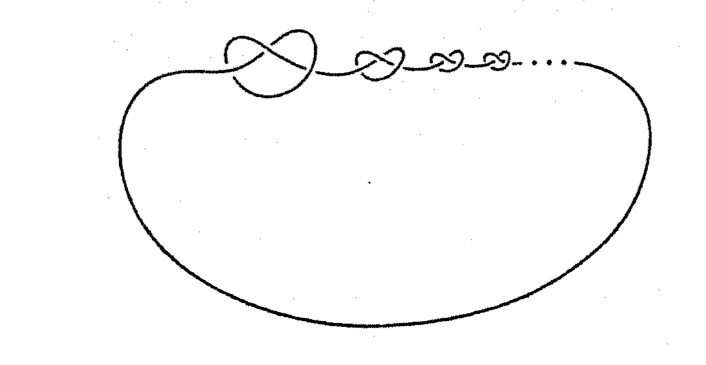
\includegraphics[scale=0.3]{1/pictures/wild.png}
% 	\end{center}
\begin{figure}[!ht]
	\centering
	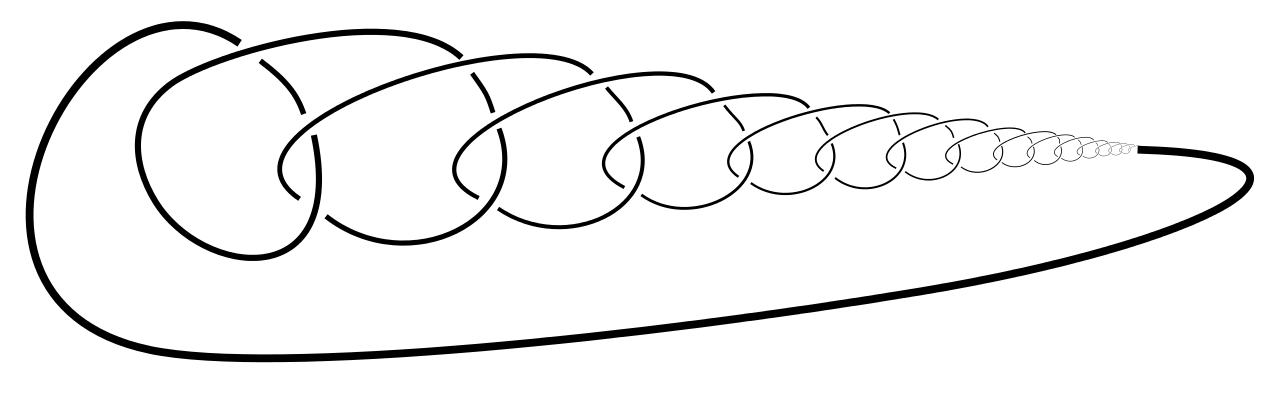
\includegraphics[scale=0.2]{img/wezeldziki.png}
	\caption{Węzeł dziki.}
	\label{fig:wezeldziki}
\end{figure}

Węzły $K$ i $J$ chcielibyśmy uważać za równoważne, jeżeli istnieje rodzina węzłów $K_t$ dla $t \in [0,1]$, taka że $K_0 = K$, $K_1 = J$ i $K_t$ powinien ,,nie różnić się'' znacznie od $K_s$ dla $s \approx t$.
Niestety umożliwia ona ściągnięcie każdej pętli do punktu.

\begin{figure}[!ht]
	\centering
	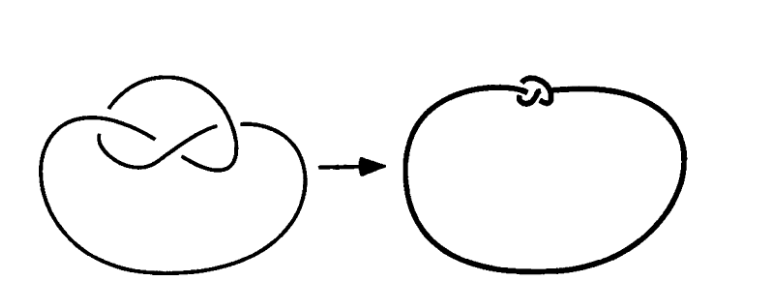
\includegraphics[scale=0.25]{img/petla.png}
	\caption{Ściągnięcie pętli.}
	\label{fig:wezeldziki}
\end{figure}

Rozwiązanie tych problemów jest zaskakująco proste: zamiast odwoływać się do pojęcia gładkiej krzywej, wystarczy posłużyć się łamaną.
Posiada ona skończenie wiele wierzchołków, więc wyklucza z rozważań dzikie węzły.
Pozwala również na podanie prostego opisu dozwolonych deformacji.

Skorzystamy z notacji $[p,q] := \{\lambda p + (1-\lambda)(q-p) : \lambda\in[0,1]\}$ dla różnych punktów $p, q \in \R^3$.
Łamaną o parami różnych wierzchołkach $p_1, \ldots, p_n \in \R^3$ jest zbiór $\bigcup_{i < n} [p_i, p_{i+1}]$.
Jeżeli $p_1 = p_n$, to łamana jest zamknięta.
Łamana jest pozbawiona samoprzecięć, kiedy każdy jej punkt naeży do dokładnie jednego odcinka postaci $[p_i, p_{i+1}]$.

\begin{definicja}
	Węzeł to łamana zamknięta w $\R^3$ bez samoprzecięć.
\end{definicja}

Zauważmy, że każdy węzeł jest jednoznacznie wyznaczony przez minimalny (w sensie zawierania) zbiór wierzchołków łamanej.

\begin{definicja}
	Splot to teoriomnogościowa suma skończenie wielu parami rozłącznych węzłów, zwanych składowymi.
\end{definicja}

\begin{przyklad}
Przykłady splotów: $\begin{tikzpicture}
	[x=0.705mm, y=0.75mm]
	\clip (-16,-10) rectangle (16,10);
	\foreach \r in {0,180}{
	\begin{scope}[rotate=\r]
		\path[TEXTARC, xshift=-13.5] (-32:9) arc (-32:300:9);
	\end{scope}}
\end{tikzpicture}$


\begin{minipage}[b]{0.24\linewidth}
\centering
\begin{tikzpicture}
	[x=0.75mm, y=0.75mm]
	\clip (-20,-10) rectangle (20,10);
	\draw[ARC] (-10,0) circle (9);
	\draw[ARC] (10,0) circle (9);
\end{tikzpicture}
\\
,,niesplot''
\end{minipage}
\begin{minipage}[b]{0.24\linewidth}
\centering
x
\\
splot Hopfa
\end{minipage}
\begin{minipage}[b]{0.24\linewidth}
\centering
\begin{tikzpicture}[x=1mm, y=1mm,]
\begin{scope}[scale=0.75]
	\clip (-17,-15) rectangle (17,15);
	\path[ARC] (-5,5) -- (5,-5);
	\foreach \r in {0,180} {
	\begin{scope}[rotate=\r]
		\path[ARC] (-8,8) .. controls (-20,20) and (-20,-20) .. (-1.5,-1.5);
		\path[ARC, rounded corners=15] (-6.5,-3.5) -- (-6.5,14) -- (6.5,14) -- (6.5,7.5);
	\end{scope}
	}
\end{scope}
\end{tikzpicture}
\\
splot Whiteheada
\end{minipage}
\begin{minipage}[b]{0.24\linewidth}
\centering
\begin{tikzpicture}[x=1mm, y=1mm,scale=0.75]
	\clip (-17,-14) rectangle (17,18);
	\foreach \r in {30,150,270}{
	\begin{scope}[rotate=\r]
		\path[ARC, xshift=-20] (-70:10) arc (-70:10:10);
		\path[ARC,xshift=-20] (35:10) arc (35:265:10);
	\end{scope}}
\end{tikzpicture}
\\
pierścienie Borromeuszy
\end{minipage}
\end{przyklad}

Zajmiemy się teraz utożsamianiem tylko pozornie różnych węzłów.

\begin{definicja}
\label{elementarne_p}
	O węźle $J$ rozpiętym na wierzchołkach $p_0, \ldots, p_n$ mówimy, że powstaje przez elementarną definicję węzła $K$ rozpiętego na $p_1, \ldots, p_n$, gdy $p_0$ nie leży na odcinku $[p_1, p_n]$, zaś przekrój trójkąta $p_0p_1p_n$ z $K$ zawiera się w $[p_1, p_n]$.
\end{definicja}

Przekształcenie odwrotne do elementarnej deformacji również jest elementarną deformacją.

% \begin{definicja}
%  Mówimy, że węzły $J$ i $K$ są równoważne, gdy istnieje skończony ciąg węzłów $K_0, K_1, \ldots, K_n$, gdzie $K_0$ = $K$, $K_n = J$, oraz $K_{i+1}$ jest elementarną
%  deformacją węzła $K_i$. 
% \end{definicja}

% Sprawdzenie, że podana relacja jest w istocie relacją równoważności pozostawiamy czytelnikowi jako proste ćwiczenie.

% Dla przykładu rozważmy dowolny $n$-kąt wypukły na płaszczyźnie. Można łatwo pokazać przez indukcję (po liczbie wierzchołków), że każdy taki wielokąt jest równoważny trójkątowi. 
% Istotnie, dla trójkąta
% teza jest oczywista. Załóżmy jej prawdziwość dla wszystkich liczb naturalnych nie większych, niż $n$. Mając dowolny $n+1$-kąt wypukły $J = (k_0, k_1, k_2, \ldots, k_n)$ łatwo się przekonać,
% że jest on elementarnym przekształceniem $n$-kąta $ K = (k_1, k_2, \ldots, k_n)$. To, że $K$ jest wielokątem wypukłym, podobnie jak to, że pierwszy warunek z definicji \ref{elementarne_p} jest spełniony, jest oczywiste.
% Drugi warunek jest spełniony, ponieważ z wypukłości $K$ zachodzi $\left([p_0,p_1]\cup [p_0, p_n]\right) \cap K = \lbrace p_1, p_n\rbrace$.

% \begin{definicja}
%  Każdy węzeł, który jest elementem klasy abstrakcji opisanej w przykładzie nazywamy niewęzłem.
% \end{definicja}
% \begin{definicja}
%  Sploten trywialnym nazywamy sumę mnogościową skończenie wielu rozłącznych niewęzłów leżących w jednej płaszczyźnie.
% \end{definicja}

% \textbf{Uwaga} W przypadku nie-splotu warunek leżenia w jednej płaszczyźnie jest istotny. Aby się o tym przekonać czytelnik może zechcieć odpowiedzieć na pytanie, 
% jak mogą leżeć względem siebie rozłączne okręgi w $\mathbb{R}^3$, a jak muszą w $\mathbb{R}^2$.

% Od tej chwili węzły równoważne będziemy uważać za tożsame, to znaczy zamiast pisać, że węzeł $J$ jest równoważny węzłowi $K$, będziemy pisać krótko $J=K$ (właśnie w taki sposób
% został powyżej zdefiniowany niewęzeł).
% Odróżniać będziemy tylko te węzły, które nie są równoważne. 

% \subsection{Diagram}
% Od początku tej pracy, z konieczności rysowaliśmy węzły (obiekty żyjące w przestrzeni trójwymiarowej) na płaszczyźnie. 
% W tym podrozdziale podamy ścisłą definicję tych dwuwymiarowych rysunków (diagramów) i pokażemy, że jeśli dwa węzły mają przedstawienie w postaci tego samego diagramu, 
% to są w istocie równoważne.

% \begin{definicja}
%  Rzutem zbioru $A\subseteq\mathbb{R}^3$ na płaszczyznę nazwiemy funkcję $p\colon A\to\mathbb{R}^2$ określoną wzorem $p(x,y,z) = (x,y)$. Kiedy $A$ jest węzłem, $p[A]$ nazywamy 
%  rzutem węzła $A$ na płaszczyznę.
% \end{definicja}


% \begin{definicja}
% \label{rzut_reg}
%  Rzutem regularnym węzła $K$ nazywamy takie rzutowanie $p$ węzła $K$ na płaszczyznę, że
%  \begin{enumerate}
%   \item dla każdego wierzchołka $v$, dla każdego $a\in K$ jeśli $p(v) = p(a)$, to $p=a$,
%   \item dla każdych $a_1, a_2, a_3$ jeśli $p(a_1)=p(a_2)=p(a_3)$, to $a_1=a_2$ lub $a_1=a_3$ lub $a_2=a_3$.
%  \end{enumerate}
% \end{definicja}

% Zakładająć, że węzeł ma regularny rzut na płaszczyznę, możemy w ścisły sposób zdefiniować pojęcie diagramu.
% Diagramem węzła $K$ nazywamy następującą modyfikację regularnego rzutu $K$ na płaszczyznę. Jeśli przeciwobrazem punktu $(x_0, y_0)$ jest zbiór dwuelementowy 
% $\lbrace a,b\rbrace$, wówczas w tym punkcie przecinają się dwa różne odcinki, które są rzutami dwóch różnych odcinków węzła $K$, powiedzmy $I_a, I_b$. 
% Ponieważ rzut $K$ jest rzutem regularnym, więc jeden z tych odcinków leży pod drugim, co oznaczamy, jak na poniższym rysunku. \\


% 	\begin{center}

% 	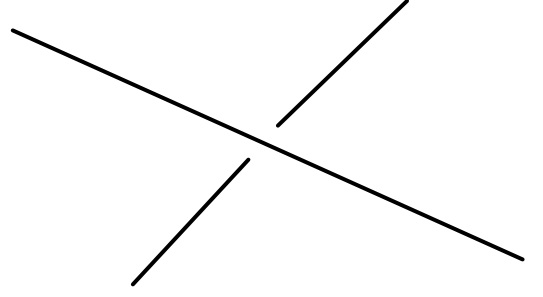
\includegraphics[scale=0.4]{1/pictures/skrz.jpg}
% 	\end{center}


% \begin{definicja}
%  Mówimy, że dwa węzły $(p_i)$, $(q_j)$ są od siebie odległe o mniej, niż $t$, gdy mają tyle samo wierzchołków i gdy dla każdej pary wierzchołków zachodzi $d(p_k,q_k) < t$.
% \end{definicja}

% Udowodnimy teraz twierdzenie, które zagwarantuje nam, że dla każdego węzła można znaleźć węzeł dowolnie mu bliski, który jest równoważny z wyjściowym, i którego rzut na płaszczyznę jest regularny. 
% Będziemy do tego potrzebować następujących lematów.

% \begin{lemat}
% \label{LEM1}
%  Dla dowolnego węzła $K = (v_0, \ldots, v_i, \ldots, v_n)$ i dowolnego $i\in\lbrace 1,2,\ldots n\rbrace$ istnieje taki $\epsilon > 0$, że dla każdego $v'\in B(v_i, \epsilon)$ 
%  węzły $K$ oraz $(v_0, \ldots,v_{i-1}, v', v_{i+1}, \ldots, v_n)$ są równoważne.
% \end{lemat}
% \begin{proof}

% Ustalmy dowolne $i$. Dodawanie i odejmowanie indeksów w dalszej części dowodu należy rozumieć jak działanie modulo $n+1$. Możemy założyć, że punkty $v_{i-1}, v_i, v_{i+1}$ nie są
% współliniowe. Zaczniemy dowód od skonstruowania dwóch stożków.
% Stożek o wierzchołku $w$, środku podstawy $s$ i promieniu podstawy $r$ będę oznaczał $S(s,r,w)$. 

% Niech $p\in\mathbb{R}^3$ będzie wektorem długości jeden prostopadłym do odcinków $I_{i-1}$ oraz $I_i$. Oznaczmy przez $\alpha$ kąt pomiędzy odcinkami 
% $I_{i-2}$ i $I_{i-1}$. 
% Dobierzmy tak małą $\mu\in\mathbb{R}^3$, żeby kąt pomiędzy $I_{i-1}$ oraz $[v_{i-1}, v_i + \mu p]$ był mniejszy od $\alpha$. Możemy $\mu$ wyliczyć np. używając trygonometrii 
% w trójkącie prostokątnym o wierzchołkach $v_{i-1}, v_i, v_i + r\cdot p$, gdzie $r\in\mathbb{R}_+$. Połóżmy
% \begin{displaymath}
%  \epsilon = \frac{1}{2}\min\lbrace d(I_{i-1}, K\setminus(I_{i-2}\cup I_i)), \mu\rbrace, \hbox{ oczywiście }\epsilon>0.
% \end{displaymath}
% Wtedy
% \begin{enumerate}
%  \item $S(v_i, \epsilon, v_{i-1})\cap K \subseteq I_{i-1}\cup I_i$,
%  \item dla każdej $\delta\in(0,\epsilon)$ zachodzi $[v_{i-1}, v_i+\delta p]\subseteq S(v_i, \epsilon, v_{i-1})$.
% \end{enumerate}
% Zauważmy, że $d(v_i, cl(K\setminus(I_{i-1}\cup I_i)) > 0$, więc (jako że $\mathbb{R}^3$ jest $T_4$) można znaleźć takie
% $\gamma > 0$, że $B(v_i,\gamma)\cap cl(K\setminus(I_{i-1}\cup I_i)) = \emptyset$. Możemy wziąć takie $\gamma$, żeby $\gamma < \epsilon$.

% Wtedy stożek 
% $S_{i-1} = S(v_i + \gamma(v_i-v_{i-1}), \epsilon, v_{i-1})$ spełnia własność $1$ oraz własność
% \begin{displaymath}
%  \hbox{dla każdego }v'\in B(v_i, \gamma) \ \ [v_{i-1}, v']\subseteq S_{i-1}.
% \end{displaymath}


% W analogiczny sposób konstruujemy stożek $S_i = S(v_i + \gamma'(v_i - v_{i+1}), \epsilon', v_{i+1})$. Zbiory $S_{i-1}$ i $S_i$ mają niepuste wnętrza, oraz 
% $v_i\in int(S_i)\cap int(S_{i+1})$. Istnieje więc taka liczba $r>0$, że $B(v_i, r)\subseteq S_i\cap S_{i+1}$.

% Owe stożki pomogą nam pokazać, że dla każdego $v'\in B(v_i, r)$ węzeł $(v_1, \ldots, v', \ldots, v_n)$ jest równoważny $K$.

% Ustalmy $v'\in B(v_i, r)$. Wtedy odcinki $[v_{i-1}, v'], [v',v_i], [v', v_{i+1}]$ należą do zbioru $S_i\cup S_{i-1}$, który jest rozłączny z $K\setminus(I_{i-1}\cup I_i)$. 
% Rozważmy dwa przypadki. 

% Jeżeli $v'\in I_i$ (gdy $v'\in I_{i-1}$, to postępujemy analogicznie), to węzeł $K$ można zdefiniować za pomocą łamanej $(v_1, \ldots, v_i, v', v_{i+1}, \ldots, v_n)$. Ponieważ
% wnętrze odcinka $[v_{i-1}, v']$ jest rozłączne z $K$, więc $K$ jest równoważny węzłowi $(v_1, \ldots, v_{i-1}, v', v_{i+1}, \ldots, v_n)$.

% Jeśli $v'\not\in I_i\cup I_{i-1}$, wówczas wnętrze odcinka $[v_i, v']$ jest rozłączne z $I_i\cup I_{i-1}$. Rozważmy odcinek $[v_{i-1}, v']$, jeśli przecina on odcinek $I_i$, to 
% wtedy odcinek $[v', v_i]$ nie przecina odcinka $I_{i-1}$, zatem bez zmniejszenia ogólności możemy założyć, że wnętrze odcinka $[v_{i-1}, v']$ jest rozłączne z $K$. Tworzymy
% następujący ciąg
% \begin{displaymath}
%  K_0 = K, K_1 = (v_1,\ldots, v_{i-1}, v', v_i, \ldots, v_n), K_2 = (v_1,\ldots, v_{i-1}, v', v_{i+1}, \ldots, v_n).
% \end{displaymath}
% Czytelnik zechce się sam przekonać, że jest to ciąg elementarnych deformacji. 
% Kładziemy $K' = K_2$ i kończymy dowód.
% \end{proof}
% \textbf{Uwaga} Ponieważ funkcja
%  $ d(x,y)\mapsto d(p(x), p(y))$ jest nierosnąca, więc przy oznaczeniach, jak w dowodzie lematu zachodzi $p(v')\in B(p(v_i),\epsilon)$.

% \begin{lemat}
%  \label{LEM2}
%  Rozpatrzmy węzeł $K = (v_1, \ldots, v_n)$. Niech $p$ oznacza rzut na płaszczyznę. Dla każdego $i$, dla każdego $\epsilon > 0$ istnieje węzeł
%  węzeł $J = (q_1, \ldots, q_i, \ldots q_n)$ równoważny węzłowi $K$ odległy od $K$ o mniej niż $\epsilon$ oraz spełniający:
%  dla dowolnego $r\in J$ i dla dowolnego $i$ zachodzi $p(q_i)\neq p(r)$, gdzie $p$ oznacza rzut prostokątny na płaszczyznę $OXY$.
% \end{lemat}
%  \begin{proof}
%   Niech $i$ będzie dowolne. 
%   Niech $\epsilon'$ będzie dobrany do wierzchołka $v_i$, jak w tezie lematu \ref{LEM1}. W razie potrzeby możemy go zmniejszyć, tak by $\epsilon'<\epsilon$. 
%   Zauważmy, że $p[B(v_i, \epsilon')] = B(p(v_i),\epsilon')$, gdzie kula po lewej stronie równości jest z $\mathbb{R}^3$, a po prawej z $\mathbb{R}^2$. Ponieważ zbiór $p(K)$ jest nigdziegęstym podzbiorem płaszczyzny, więc możemy wybrać taki $q_i\in B(v_i, \epsilon')$,
%   że $p[\lbrace q_i\rbrace]\cap p[K] = \emptyset$. Otrzymujemy w ten sposób nowy węzeł $(v_1, \ldots, q_i, \ldots, v_n)$. Powtarzamy opisaną procedurę $n-1$ razy i w efekcie 
%   otrzymujemy węzeł $J$. Ponieważ $\epsilon'$ był z lematu \ref{LEM1}, więc $J$ i $K$ są równoważne. 
%  \end{proof}


% \begin{twierdzenie}
%  Niech $K$ będzie węzłem o uporządkowanym zbiorze wierzchołków $(v_1, v_2, \ldots, v_n)$. Dla każdego $\epsilon > 0$ istnieje węzeł $K'$, 
% który jest odległy od węzła $K$ o nie więcej, niż $\epsilon$, oraz jego rzut na płaszczyznę $OXY$ jest regularny. 
% \end{twierdzenie}
% \begin{proof}

% Najpierw zastosujemy lemat \ref{LEM2} do węzła $K$ i powstały w ten sposób węzeł oznaczymy przez $K'$.

% Ponieważ rzut węzła $K'$ spełnia pierwszy warunek z definicji \ref{rzut_reg}, więc dla dwóch różnych odcinków $I,J$ węzła 
% $K'$ zachodzi $|p(I)\cap p(J)| \le 1$.

% Niech $\mathcal{A}$ będzie rodziną wszystkich takich podzbiorów zbioru odcinków węzła $K'$, że dla każdego $A\in\mathcal{A}$ zachodzi 
% \begin{enumerate}
%  \item $|A| > 1$,
%  \item istnieje taki $r\in\mathbb{R}^2$, że $\bigcap_{I\in A}p(I) = \lbrace r\rbrace$,
%  \item dla każdego $J\not\in A$ $\left(\bigcap_{I\in A}p(I)\right)\cap p(J) = \emptyset$.
% \end{enumerate}

% Niech $a\in K'$ będzie punktem z wnętrza pewnego odcinka $I_i$, takim że istnieją różne od $a$ punkty $b, c\in K'$ takie że $p(a) = p(b) = p(c)$ i $b\neq c$. 
% Niech $\lbrace t_A\rbrace_{A\in\mathcal{A}}$ będzie ciągiem w $\mathbb{R}^2$, takim że $t_A = \bigcap_{I\in A}p(I)$. Niech $u\in\mathbb{R}^2$ będzie niezerowym wektorem prostopadłym do osi $OZ$, który
% nie jest równoległy do $p(I_{i-1})$ oraz nie jest równoległy do $p(I_{i+1})$. Wtedy, używając tego samego argumentu, co w dowodzie lematu \ref{LEM2}, możemy znaleźć dostatecznie małą $\delta > 0$, że dla każdej $0 < \delta' < \delta$ istnieje wektor $w$, taki że
% węzeł $(v_1, \ldots, v_{i-1}, v_i  + \delta'w, v_{i+1}  + \delta'w, v_{i+2}, \ldots, v_n)$ jest równoważny węzłowi $K'$, oraz rzut tego węzła spełnia punkt pierwszy 
% defnicji \ref{rzut_reg}. Ponieważ ciąg $t_A$ jest skończony, to
% liczbę $\delta'$ można wziąć na tyle małą, żeby była mniejsza od dowolnej dodatniej odległości $d(p(I_j), t_A)$ dla $j \in \lbrace i-1, i+1\rbrace$.
% Wtedy węzeł powstały z $K'$ przez zastąpienie $v_i, v_{i+1}$ wierzchołkami $v_i'=v_{i} + \delta'w, v_{i+1}'=v_{i+1}+\delta'w$
% odpowiednio jest równoważny węzłowi $K'$, co więcej, dla każdego $r\in[v_{i-1}, v_i']\cup[v_i', v_{i+1}']\cup[v_{i+1}', v_{i+2}]$ istnieje co najwyżej jeden taki $r'\neq r$, że $p(r') = p(r)$.
% Zauważmy, że po tej zastosowaniu tej procedury przynajmniej jeden element rodziny $\mathcal{A}$ ma jeden element mniej.
% zatem w skończonej liczbie kroków dojdziemy do momentu, kiedy w rodzinie $\mathcal{A}$ zostaną jedynie zbiory dwuelementowe. Wtedy rzut otrzymanego węzła będzie regularny. 

% \end{proof}


% Warto podkreślić, że dwa różne węzły (w sensie relacji równości) mogą mieć ten sam diagram, np. mając dany węzeł można przesunąć jego wierzchołek o największej trzeciej współrzędnej 
% o wersor równoległy do osi $OZ$. Okazuje się jednak, że jeśli dwa węzły mają ten sam diagram, to są równoważne. 


% \begin{twierdzenie}
%  Jeśli dwa węzły $K = (v_1,\ldots, v_n)$ oraz $W = (w_1, \ldots, w_n)$ mają regularne rzutowanie oraz ich diagramy są równe, to $K$ i $J$ są równoważne.
% \end{twierdzenie}
% \begin{proof}
%  Ustalmy wierzchołek $v_i$. Zauważmy, że bez straty ogólności możemy założyć, że rzut każdego z odcinków $I_i, I_{i-1}$ węzła $K$ zawiera co najwyżej jedno skrzyżowanie. 
%  Istotnie, jeśli
%  rzut odcinka $I_i$ zawiera więcej skrzyżowań (oczywiście jest ich skończenie wiele), to niech $s_0$ oznacza skrzyżowanie najbliższe $p(v_i)$, a $s_1$ skrzyżowanie najbliższe
%  punktowi $s_0$. Wybierzmy dowolny punkt z wnętrza odcinka $[s_0, s_1]$, oznaczmy go przez $s$. Niech $v' = p^{-1}(s)$. Wtedy łamana $(v_1, \ldots, v_i, v', v_{i+1})$ definiuje 
%  węzeł $K$. Wówczas odcinek $p[ [v_i, v']]$ zawiera dokładnie jedno skrzyżowanie. To samo możemy założyć o węźle $J$ dodając nowy wierzchołek $q'$ w punkcie $p^{-1}(s)$.
 
%  Niech $I, J$ oznaczają te odcinki węzła $K$, że $p[I]\cap p[I_i]\neq\emptyset$ oraz $p[J]\cap p[I_{i-1}]\neq\emptyset$. Wtedy $I$ leży ,,pod'' odcinkiem $I_i$ i pod odcinkiem
%  węzła $W$, który jest rzutowany na $p[I_i]$, albo ,,nad'' oboma tymi odcinkami. To samo się tyczy odcinka $J$. Stąd wynika, że wnętrza odcinków $[v_{i-1}, w_i], [w_i, v_{i+1}]$ są
%  rozłączne z węzłem $K$. To, że $K\cap [v_i,w_i] = \lbrace v_i\rbrace$ jest oczywiste. Dlatego ciąg
%  \begin{displaymath}
%   K_0 = (v_1, \ldots, v_n), K_1 = (v_1, \ldots, v_{i-1}, w_i, v_i, v_{i+1}, \ldots, v_n), K_3 = (v_1, \ldots, v_{i-1}, w_i, v_{i+1}, \ldots, v_n)
%  \end{displaymath}
% jest ciągiem elementarnych deformacji. Stosując powyżej opisaną procedurę do każdego wierzchołka węzła $K$ otrzymamy na końcu węzeł $J$, co znaczy, że te węzły są równoważne.
 
%  \end{proof}

% \subsection{Każdy kij ma dwa końce, czyli orientacja węzła}
% Jak już wcześniej zostało powiedziane, węzeł to łamana w $\mathbb{R}^3$. Łamana z kolei jest wyznaczona jednoznacznie przez zbiór  swoich wierzchołków. Mając dany węzeł o wierzchołkach
% $(v_1, v_2, \ldots, v_n)$, możemy go zorientować, to znaczy dla każdego odcinka węzła wybrać początek i koniec tego odcinka. Chcielibyśmy to zrobić w taki sposób, żeby każdy wierzchołek
% był końcem dokładnie jednego odcinka. W tym sensie węzeł $(v_1, v_2, \ldots, v_n)$ jest węzłem różnym od węzła $(v_n, \ldots, v_2, v_1)$, mimo, że jako podzbiory $\mathbb{R}^3$ są
% sobie równe. Teraz spróbujemy sformalizować to, co dotychczas powiedzieliśmy.

% \begin{definicja}
%  Odcinkiem zorientowanym w $\mathbb{R}^3$ o początku w $p$ i końcu w $q$ (zakładamy, że $p\neq q$) nazywamy liniowe włożenie $l\colon[0,1]\to\mathbb{R}^3$, takie że $l(0) = p, l(1) = q$ i oznaczamy przez
%  $[p,q]_o$. 
% \end{definicja}

% Innymi słowy odcinek zorientowany to odcinek z wyróżnionym początkiem i końcem. Co więcej, przy oznaczeniach z definicji zachodzi
% \begin{displaymath}
%  q-p =  |q-p|\cdot\frac{l'(x)}{|l'(x)|}, \hbox{ dla dowolnego } 0 < x < 1.
% \end{displaymath}

% \begin{definicja}
%  Orientacją węzła $K = (v_1, v_2, \ldots, v_n)$ nazywamy takie zorientowanie jego odcinków, że każdy wierzchołek jest końcem (równoważnie - początkiem) dokładnie jednego odcinka.
% \end{definicja}

% Nie trudno się przekonać, że każdy węzeł można zorientować na dokładnie dwa sposoby. Istotnie, wybranie orientacji jednego odcinka węzła jednoznacznie wyznacza orientacje całego
% węzła. 

% Przyjmiemy następującą konwencję, jeśli powiemy, że węzeł $K = (v_1, v_2, \ldots, v_n)$ jest węzłem zorientowanym, będziemy przez to rozumieć, że $I_1 = [v_1, v_2]_o$.

% \textbf{Uwaga} Niech będzie dany węzeł $K = (v_1, v_2, \ldots, v_n)$, niech ponadto uporządkowane $n$-tki $K_i = (v_{i_1}, v_{i_2}, \ldots, v_{i_n})$ 
% oraz $K_j = (v_{j_1}, v_{j_2}, \ldots, v_{j_n})$ definiują ten sam węzeł $K$. Niech $O_i, O_j$ oznaczają orientację zorientowanych węzłów $K_i, K_j$ odpowiednio. Powiemy, że orientacja
% $O_i$ jest równoważna orientacji $O_j$, gdy isnieje taka $\sigma\in S_n$, że dla każdego $k$ zachodzi $\sigma(i_k) = j_k$. Sprawdzenie, że ta relacja jest w istocie relacją równoważności
% pozostawiamy jako proste ćwiczenie. 

% \begin{definicja}
%  Węzłem zorientowanym nazywamy węzeł z wybraną orientacją.
% \end{definicja}

% Elementarne deformacje węzła zorientowanego definiuje się w sposób oczywisty. Do zestawu punktów $(1), (2)$ z definicji \ref{elementarne_p} należy dodać następujący warunek.
% \begin{displaymath}
%  \hbox{Odcinki zorientowane koincydentne z wierzchołkiem } p_0 \hbox{ są równe }[p_n, p_0]_o, [p_0, p_1]_o.
% \end{displaymath}

% \begin{definicja}
%  Węzły zorientowane nazywamy równoważnie zorientowanymi, gdy w skończenie wielu krokach za pomocą elementarnych deformacji jednego węzła zorientowanego
%  możemy otrzymać drugi.
% \end{definicja}
% Należy wyraźnie powiedzieć, że równoważność dwóch węzłów jest istotnie inną relacją, niż równoważność węzłów w sensie orientacji. Istnieją bowiem przykłady węzłów równoważnych
% ale nie równoważnych w sensie orientacji. Opisanie ich dokładnie wykracza jednak poza możliwości intelektualne autora, dlatego fakt ten, z wyższej konieczności, jest podany
% czysto informacyjnie. 
% Na koniec tego rozdziału podamy jeszcze jedną definicję.
% \begin{definicja}
%  Odwrotnością węzła zorientowanego $K = (v_1, v_2, \ldots, v_n)$ nazywamy węzeł $K^r = (v_n, v_{n-1}, \ldots, v_1)$. Powiemy, że $K$ jest węzłem odwracalnym, jeżeli $K$ i $K^r$ są
%  równoważne w sensie orientacji. Dla węzła $J$ niezorientowanego, powiemy że jest on odwracalny, jeśli istnieje taka orientacja węzła $J$, że jest on odwracalny (jako węzeł
%  zorientowany z tą wybraną orientacją).
% \end{definicja}


% \subsection{Ruchy Reidemeistera}
% W tym podrozdziale przedstawimy pierwsze poważne narzędzie, które w wielu przypadkach pozwoli nam rozstrzygnąć, czy dwa węzły są równoważne, czy też nie. 
% Na początku sformuujemy nową definicję elementarnej deformacji, równoważną tej, którą wpprowadziliśmy wcześniej.

% \begin{definicja}
% \label{wygoda}
%  Węzeł $K'$ jest elementarną deformacją węzła $K = (v_1,, v_2, \ldots, v_n)$, gdy
%  \begin{enumerate}
%   \item $K'=(v_1, v_2, \ldots, v_i, v', v_{i+1}, \ldots, v_n)$, gdzie $v'\in \hbox{Int}I_i$, lub
%   \item $K' = (v_1, v_2, \ldots, v_{i-1}, v', v_{i+1}, \ldots, v_n)$, o ile czworokąt $C$ o wierzchołkach $v_{i-1}, v_i, v_{i+1}, v'$ spełnia $C\cap K = I_{i-1}\cup I_i$.
%  \end{enumerate}
%  Równoważność tej definicji z definicją podaną wcześniej jest oczywista.
% \end{definicja}

% \begin{definicja}
%  Następujące trzy operacje (wraz z operacjami odwrotnymi - w sumie jest ich sześć) nazywamy ruchami Reidemaistera.
 
% 	\begin{enumerate} 

% \item Pierwszy ruch Reidemeistera: 
	
% 	\begin{minipage}{0.5\textwidth}
% 		\begin{center}
% 			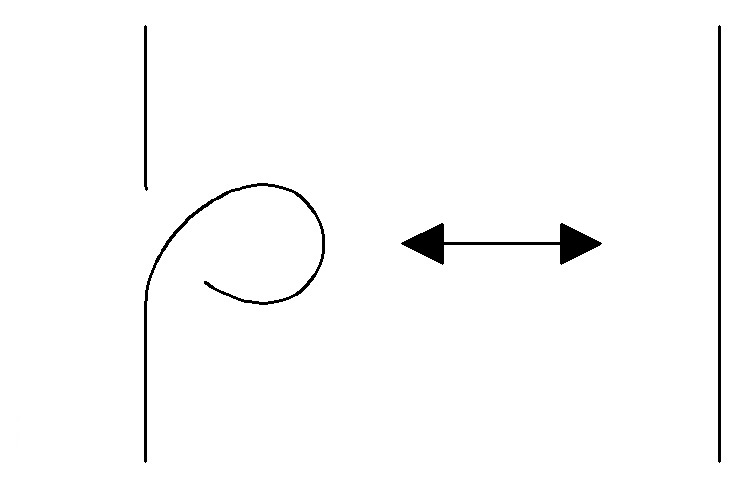
\includegraphics[scale=0.2]{1/pictures/R1}
% 		\end{center}
% 	\end{minipage}
% \item Drugi ruch Reidemeistera: 

% 	\begin{minipage}{0.5\textwidth}
% 		\begin{center}
% 			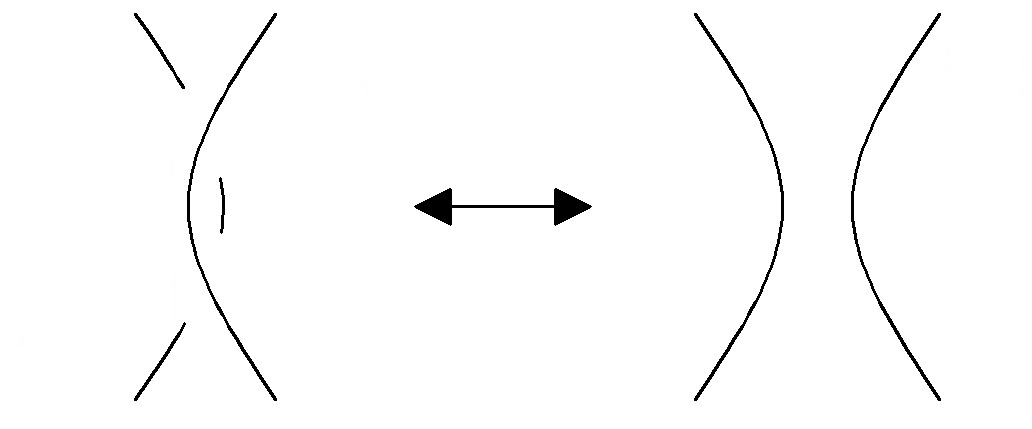
\includegraphics[scale=0.2]{1/pictures/R2}
% 		\end{center}
% 	\end{minipage}
	
% \item Trzeci ruch Reidemeistera: 

% 	\begin{minipage}{0.65\textwidth}
% 		\begin{center}
% 			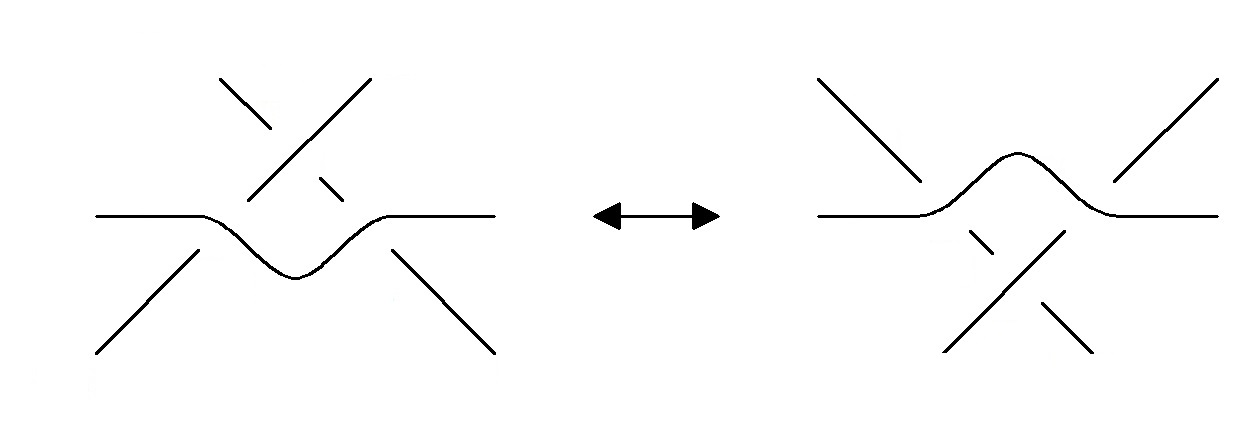
\includegraphics[scale=0.25]{1/pictures/R3}
% 		\end{center}
% 	\end{minipage}
	
% 	\end{enumerate}
 
% \end{definicja}

% \begin{definicja}
%  Dwa diagramy uważa się za równoważne, gdy za pomocą skończonej liczby ruchów Reidemeistera z jednego diagramu można otrzymać drugi.
% \end{definicja}

% \begin{twierdzenie}{(Reidemeister'a)}
% Dwa węzły są równoważne, wtedy i tylko wtedy, gdy ich diagramy są równoważne.
% \end{twierdzenie}

% \begin{proof}

% Załóżmy najpierw, że mamy dane węzły $J$ i $K$, oba te węzły mają regularny rzut na płaszczyznę, oraz węzeł $K$ można otrzymać z węzła $J$ przez pewien ciąg elementarnych deformacji.
% Ponieważ ten ciąg jest skończony, bez zmniejszenia ogólności możemy założyć, że węzeł $K$ powstaje z węzła $J$ w wyniku jednej elementarnej deformacji. Wystarczy więc pokazać, że 
% ta deformacja odpowiada ciągowi ruchów R na diagramie węzła $J$. 

% Rozważmy pojedynczą elementarną deformację węzła $J$ w sensie definicji \ref{wygoda}. Powiedzmy że $J = (v_1, \ldots, v_{i-1}, v_i, v_{i+1}, \ldots, v_n)$, oraz że 
% $K = (v_1, \ldots, v_{i-1}, v', v_{i+1}, \ldots, v_n)$. Ogólny przypadek na pierwszy rzut wydaje się być mocno skomplikowany. Opiszemy go za pomocą wielu podprzypadków, z którymi
% w prosty sposób potrafimy sobie poradzić. 

% Niech $C$ oznacza czworokąt $v_{i-1}, v_i, v_{i+1}, v'$, przez $o$ oznaczmy odcinek $vv'$. Przez $S$ oznaczmy zbiór skrzyżowań z wnętrza $C$ (jako podzbiór $\mathbb{R}^2$), 
% przez $W$ oznaczmy zbiór wierzchołków z wnętrza $C$, przez $P$ oznaczmy zbiór punktów przecięcia osi $o$ z łukami z wnętrza $C$. 
% Oczywiście zbiór $S\cup W\cup P$ jest skończony. Niech $A$ oznacza obraz tego zbioru przez rzut promienisty na $o$, to znaczy, jeśli dany punkt $p$ jest po tej samej stronie osi $o$, 
% co punkt $v_{i-1}$($v_{i+1}$), to rzutem promienistym punktu $p$ na $o$ nazwiemy rzutowanie na $o$ w kierunku prostej zawierającej odcinek $[p, v_{i-1}]$($[p, v_{i+1}]$). 
% Możemy założyć, że rzuty punktów z $S\cup W\cup P$ są parami różne, oraz że żadne skrzyżowanie ani wierzchołek nie leżą na osi $o$.
% Jeśli by tak nie było, możemy używając drugiego ruchu R odrobinę poprzesuwać skrzyżowania i miejsca przecięcia łuków z osią. 
% Niestety w przypadku, kiedy skrzyżowanie i wierzchołek znajdują się na prostej, wzdłuż której odbywa się rzutowanie, sytuacja jest nieco bardziej skomplikowana, co widać na poniższym
% rysunku.



% 	\begin{center}

% 	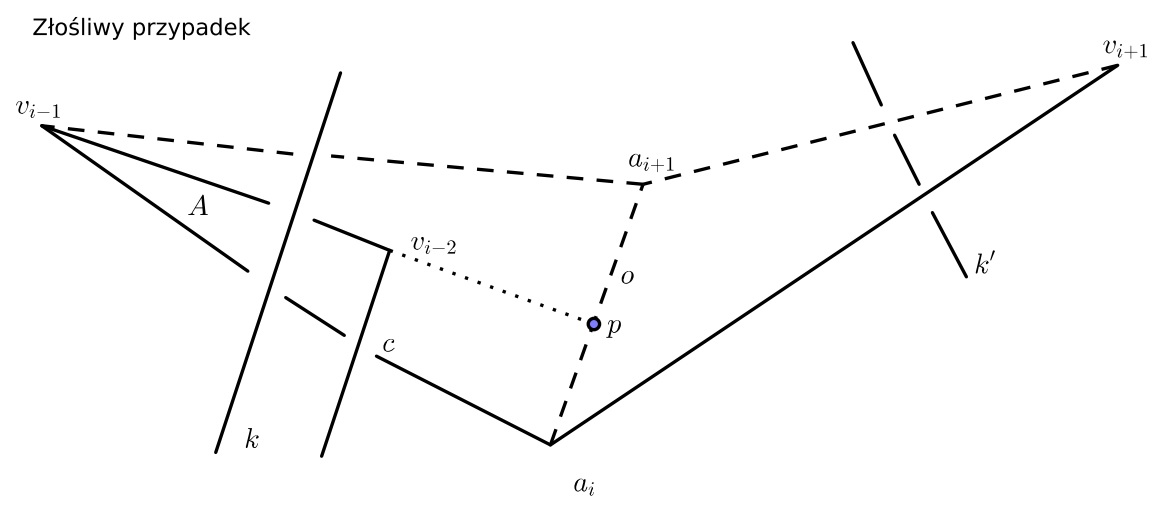
\includegraphics[scale=0.5]{1/pictures/bad.jpg}
% 	\end{center}


% Oczywiście łuków złośliwych w sensie złośliwości łuku $k$ może być więcej, niż jeden (bez zmniejszenia ogólności możemy założyć, że wewnątrz $C$ nie ma skrzyżowań - 
% to założenie będzie łatwo wynikać z dalszej części dowodu), ale będzie istniał taki, którego skrzyżowanie z $I_{i-1}$ będzie najbliżej wierzchołka $v_{i-2}$.
% Radząc sobie z tym delikwentem, oraz używając indukcji (skończonej), jesteśmy w stanie poradzić sobie z przypadkiem, kiedy złośliwych łuków jest dowolnie wiele. To jednak nie wyczerpuje
% wszystkich tego typu przypadków. Istnieje kilka podobnych (ale nie jest ich wiele, pamiętajmy, że $C$ ma być rozłączny z resztą węzła), np. łuk $k$ przechodzi pod czworokątem $C$, a odcinki $I_{i-2}, I_{i-1}$ przechodzą pod $k$. 
% Ponieważ wszystkie te przypadki są bardzo podobne, tu opiszemy tylko jeden, a resztę zostawiamy czytelnikowi jako nietrudne ćwiczenie.
% Aby poradzić sobie z przypadkiem przedstawionym na rysunku powyżej, należy najpierw łuk $k$ przenieść na drugą stronę skrzyżowania $c$ (trzeci ruch R), potem cofnąć wierzchołek $v_{i-2}$
% tak, żeby znajdował się bliżej wierzchołka $v_{i-1}$ niż łuk $k$ przed przesunięciem (tu nam pomoże drugi ruch R zastosowany parokrotnie), 
% następnie wrócić łuk $k$ na jego pierwotne miejsce (znów trzeci ruch R).
 

% Niech $B$ oznacza zbiór zrzutowanych punktów na oś $o$. Wprowadżmy na $o$ następującą relację porządku: $x < y\iff d(v_i,x) < d(v_i, y)$. Ustawmy zbiór $B$ rosnąco $x_1, x_2, \ldots, x_{l-1}$.
% Niech $v_i = a_0, a_1, a_2, \ldots, a_l = v'$ będzie ciągiem punktów, takim że $a_i\in o$, oraz $x_i < a_i < x_{i+1}$ w sensie wprowadzonego porządku. 
% Wystarczy zatem pokazać, że każdą z elementarnych deformacji przeprowadzających wierzchołek $v_i$ na $a_1$, wierchołek $a_1$ na punkt $a_2$, $\ldots$, 
% wierzchołek $a_{l-1}$ na punkt $a_l$ można uzyskać za pomocą sekwencji ruchów R, co prowadzi do rozbicia problemu na wiele mniejszych podprzypadków, których lista znajduje się
% poniżej.


% 	\begin{center}

% 	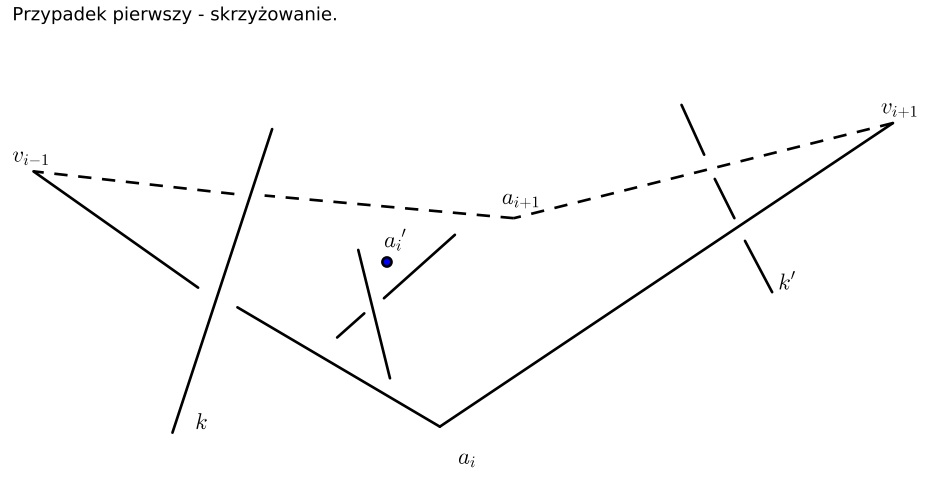
\includegraphics[scale=0.6]{1/pictures/cross.jpg}
% 	\end{center}

% Łuki skrzyżowania mogą przechodzić, albo oba nad bokami czworokąta $C$, albo oba pod bokami $C$, albo jeden może leżeć nad czworokątem, a drugi pod. Dwa pierwsze przypadki są oczywiste,
% radzimy sobie z nimi stosując trzeci ruch R, oraz w celach kosmetycznych drugi ruch R. Trzeci przypadek jest nieco trudniejszy, ale również główną rolę gra w nim trzeci ruch R. Po
% prostu można przenieść łuk, który przechodzi nad czworokątem $C$ na drugą stronę skrzyżowania łuku przechodzącego pod czworokątem $C$ i łuku $a_i v_{i-1}$, potem parokrotnie zastosować
% drugi ruch R a na koniec znów zastosować trzeci ruch R, żeby przenieść łuk, który ruszyliśmy na początku, na jego pierwotne miejsce.


% 	\begin{center}

% 	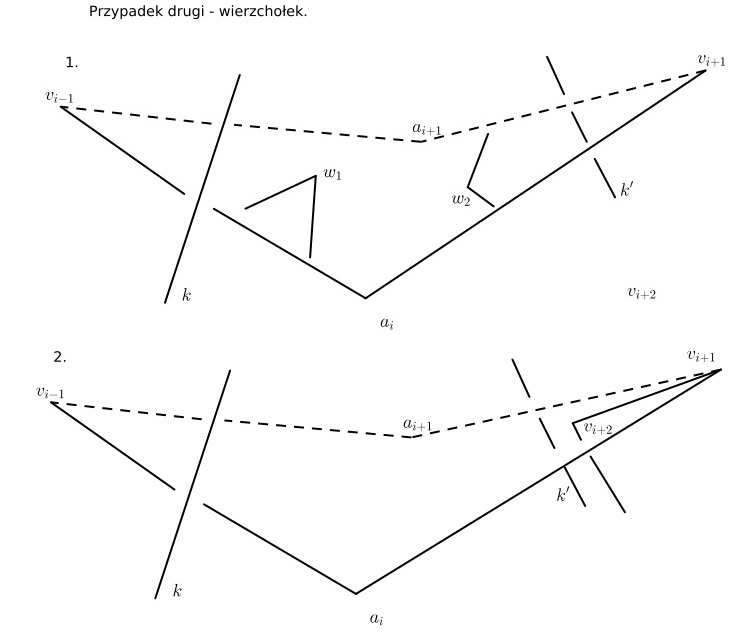
\includegraphics[scale=0.8]{1/pictures/vertex.jpg}
% 	\end{center}

	
% Podprzypadek pierwszy jest prosty, wystarczy zastosować drugi ruch R. Przypadek drugi wymaga nieco komentarza. 

% Żeby poradzić sobie z przypadkiem 2. należy zastosować pierwszy ruch R (wcześniej go nie stosowaliśmy) do pętli $a_iv_{i+1}v_{i+2}$. To nam pozwoli wyrzucić wierzchołek $v_{i+2}$ z 
% czworokąta $C$. Mamy też pewność, że efektem ubocznym tego ruchu nie będą żadne nowe skrzyżowania, ani wierzchołki, ani łuki przecinające oś $o$, zatem będziemy w stanie przenieść 
% wierzchołek $a_i$ na wierzchołek $a_{i+1}$. Na koniec, musimy wykonać operację odwrotną do tej, która wyrzuciła wierzchołek $v_{i+2}$ z czworokąta $C$, która sprawi, że $v_{i+2}$
% wróci na swoje pierwotne miejsce.


% 	\begin{center}

% 	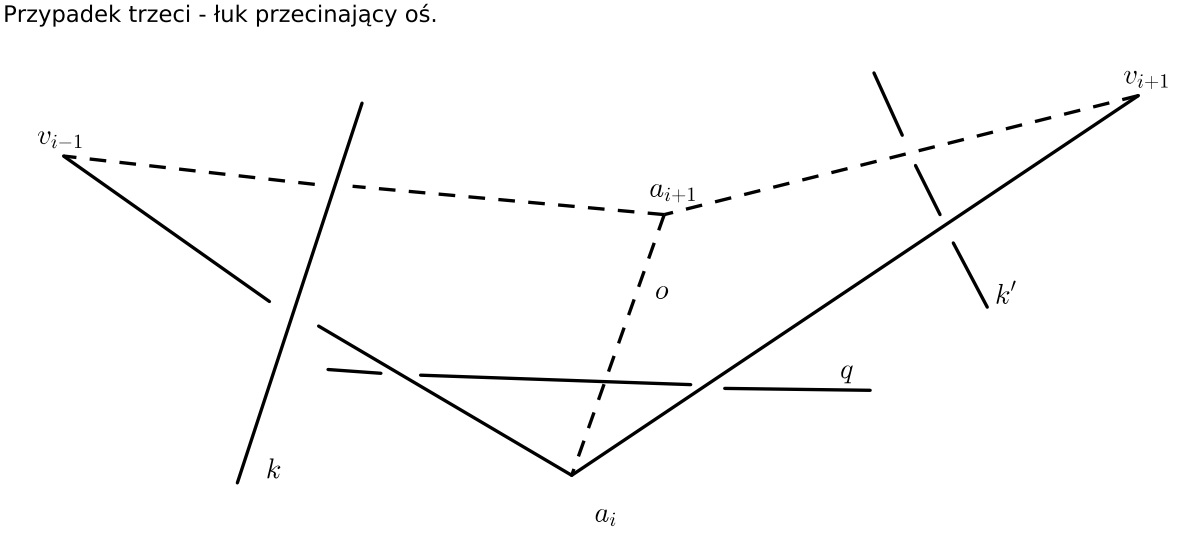
\includegraphics[scale=0.5]{1/pictures/axis.jpg}
% 	\end{center}

	
% Ten przypadek jest prosty, żeby przenieść wierzchołek $a_i$ na drugą stronę łuku $q$ wystarczy zastosować drugi ruch R. Przypadek, kiedy łuk $q$ przechodzi nad czworokątem $C$ jest analogiczny.

% Na koniec trzeba jeszcze pamiętać o naszym początkowym założeniu o tym, że rzuty są parami różne, i że żadne skrzyżowania, ani wierzchołki nie leżą na osi $o$. Jeśli potrzebowaliśmy
% lekko zmodyfikować diagram wyjściowego węzła, żeby to założenie było prawdziwe, musimy na koniec wykonać modyfikacje odwrotne, które oczywiście można uzyskać za pomocą ruchów R.

% W ten sposób zakończyliśmy szkic dowodu implikacji w jedną stronę. Implikacja w drugą stronę jest oczywista. 
	
% \end{proof}

\begin{definicja}
Węzeł to łamana w $\mathbb{R}^3$ bez samoprzecięć.
\end{definicja}

\end{document}		

\documentclass[12pt,oneside,reqno,notitlepage]{article}

% Packages
\usepackage{amssymb,amsmath,amsthm}
\usepackage{verbatim}
\usepackage[]{hyperref} %hidelinks

% Page dimensions
\usepackage{geometry}
\addtolength{\textheight}{2cm}
\addtolength{\topmargin}{-1cm}

% Font
\usepackage{mathptmx}
\DeclareSymbolFont{cmlargesymbols}{OMX}{cmex}{m}{n}

% Environments
\newtheorem{lemma}{Lemma}
\newtheorem{theorem}[lemma]{Theorem}
\newtheorem{proposition}[lemma]{Proposition}
\newtheorem{corollary}[lemma]{Corollary}
\newtheorem*{theorem*}{Theorem}
\theoremstyle{definition}
\newtheorem{definition}[lemma]{Definition}
\newtheorem{quiz}[lemma]{Quiz}
\newtheorem{remark}[lemma]{Remark}
\newtheorem{rks}[lemma]{Remarks}
\newtheorem{example}[lemma]{Example}
\newtheorem{note}[lemma]{Note}
\numberwithin{lemma}{section}

%Symbols
\newcommand{\C}{\mathbb C}
\newcommand{\N}{\mathbb N}
\newcommand{\Q}{\mathbb Q}
\newcommand{\R}{\mathbb R}
\newcommand{\Z}{\mathbb Z}
\newcommand{\lk}{\mathit{lk}}
\newcommand{\col}{\mathit{Col}}
\newcommand{\Span}{\mathit{span}}

%Tikz 
\usepackage{tikz}
\usetikzlibrary{decorations.markings,external}
\tikzset{
->-/.style={decoration={markings, mark=at position .5 with {\arrow{>}}},postaction={decorate}},
-<-/.style={decoration={markings, mark=at position .5 with {\arrow{<}}},postaction={decorate}},
ARC/.style ={draw=black,line join=miter,line cap=butt,miter limit=4.00,line width=0.5 mm},
TEXTARC/.style ={draw=black,line join=miter,line cap=butt,miter limit=4.00,line width=0.3 mm},
REGION/.style={draw=none, fill=white!#1!black},
REGION/.default = 80,
}
\colorlet{darkblue}{blue!80!black}
\tikzsetexternalprefix{figures/}
\tikzexternalize
%\tikzset{external/force remake=true}

%Specific TikZ Commands
\newcommand{\RightCrossing}
	{
	\begin{tikzpicture}[scale=0.03, baseline=-3]
		\path[TEXTARC] (-5,-5) -- (5,5);
		\path[TEXTARC] (5,-5) -- (2,-2);
		\path[TEXTARC] (-5,5) -- (-2,2);
	\end{tikzpicture}
	}
\newcommand{\LeftCrossing}
	{
	\begin{tikzpicture}[scale=0.03, baseline=-3]
		\path[TEXTARC] (5,-5) -- (-5,5);
		\path[TEXTARC] (-5,-5) -- (-2,-2);
		\path[TEXTARC] (5,5) -- (2,2);
	\end{tikzpicture}
	}
\newcommand{\RightSmoothing}{
	\begin{tikzpicture}[scale=0.03, baseline=-3]
		\path[TEXTARC] (-5,-5) .. controls (-1,-1) and (-1,1) .. (-5,5);
		\path[TEXTARC] (5,-5) .. controls (1,-1) and (1,1) .. (5,5);
	\end{tikzpicture}
	}
\newcommand{\LeftSmoothing}{
	\begin{tikzpicture}[scale=0.03,baseline=-3]
		\path[TEXTARC] (-5,-5) .. controls (-1,-1) and (1,-1) .. (5,-5);
		\path[TEXTARC] (-5,5) .. controls (-1,1) and (1,1) .. (5,5);
	\end{tikzpicture}
	}
\newcommand{\UnKnot}{
	\begin{tikzpicture}[scale=0.03,baseline=-3]
		\path[TEXTARC] (0,0) circle (5);
	\end{tikzpicture}
	}
\newcommand{\ScriptRightCrossing}
	{
	\begin{tikzpicture}[scale=0.02, baseline=-2.5]
		\path[TEXTARC] (-5,-5) -- (5,5);
		\path[TEXTARC] (5,-5) -- (2,-2);
		\path[TEXTARC] (-5,5) -- (-2,2);
	\end{tikzpicture}
	}
\newcommand{\ScriptLeftCrossing}
	{
	\begin{tikzpicture}[scale=0.02, baseline=-2.5]
		\path[TEXTARC] (5,-5) -- (-5,5);
		\path[TEXTARC] (-5,-5) -- (-2,-2);
		\path[TEXTARC] (5,5) -- (2,2);
	\end{tikzpicture}
	}
\newcommand{\ScriptRightSmoothing}{
	\begin{tikzpicture}[scale=0.02, baseline=-2.5]
		\path[TEXTARC] (-5,-5) .. controls (-1,-1) and (-1,1) .. (-5,5);
		\path[TEXTARC] (5,-5) .. controls (1,-1) and (1,1) .. (5,5);
	\end{tikzpicture}
	}
\newcommand{\ScriptLeftSmoothing}{
	\begin{tikzpicture}[scale=0.02,baseline=-2.5]
		\path[TEXTARC] (-5,-5) .. controls (-1,-1) and (1,-1) .. (5,-5);
		\path[TEXTARC] (-5,5) .. controls (-1,1) and (1,1) .. (5,5);
	\end{tikzpicture}
	}	
\newcommand{\ScriptUnKnot}{
	\begin{tikzpicture}[scale=0.02,baseline=-2.5]
		\path[TEXTARC] (0,0) circle (5);
	\end{tikzpicture}
	}

%Invisible-able comments
\newcommand\aside[1]{}
%\newcommand\aside[1]{{\color{red} #1}}










\date{}

\begin{document}



\begin{center}
{\Huge\bf MX4540: Knots}
\\[15 pt]
{\large Notes by Richard Hepworth}
\end{center}



\section{An introduction to knots and links}


\subsection{
Knots and links}

\begin{definition}\label{knot:def}
A \emph{knot} $K\subseteq\R^3$ is a subset of the form $K=f(\R)$ where
$f\colon \R\to\R^3$ is a map with the following properties.
\begin{enumerate}
\item
$f(t_1)=f(t_2)$ if and only if $t_1-t_2\in\Z$.
\item
$f$ is smooth, so that $\mathrm{d}^nf/\mathrm{d}t^n$ exists for all $n\in\N$.
\item
$(\mathrm{d}f/\mathrm{d}t)(t)\neq 0$ for all $t\in\R$.
\end{enumerate}
(The first condition means that $f$ determines an injective map from the circle
into $\R^3$.  The second and third conditions ensure that the knot is embedded
`nicely' in $\R^3$.)
\end{definition}


\begin{example}\label{Knots:Example}
The picture below shows several knots.
\\
\begin{minipage}[b]{0.2\columnwidth}
\centering
\begin{tikzpicture}[x=0.75mm, y=0.75mm]
	\clip (-13,-13) rectangle (13,13);
	\draw[ARC] (0,0) circle (12);
\end{tikzpicture}\\
unknot
\end{minipage}
\begin{minipage}[b]{0.2\columnwidth}
\centering
\begin{tikzpicture}
[x=0.75mm, y=0.75mm]
	\clip (-18,-14) rectangle (18,20);
	\foreach \x in {270,30, 150}
		\path[ARC] (15+\x:6) .. controls (130+\x:25) and (200+\x:25) .. (225+\x:10);
\end{tikzpicture}\\
trefoil
\end{minipage}
\begin{minipage}[b]{0.2\columnwidth}
\centering
\begin{tikzpicture}
[x=0.75mm, y=0.75mm]
	\clip (-17,-15) rectangle (17,15);
	\path[ARC] (0,10) .. controls (10,0) and (-10,0) .. (0,-10);
	\foreach \d in {0,180} {
	\path[ARC, rotate=\d] (-1.5,1.5) .. controls (-6,6) and (-3,17) .. (10,12)
	.. controls (23,7) and (15,-20)  .. (3,-13);}
\end{tikzpicture}\\
also the trefoil
\end{minipage}
\begin{minipage}[b]{0.2\columnwidth}
\centering
\begin{tikzpicture}
[x=0.75mm, y=0.75mm]
	\clip (-21,-17) rectangle (21,22);
	\path[ARC] (0,-10) .. controls (8,0) and (-8,0) .. (-8,8);
	\path[ARC] (-8,12) .. controls (-8,20) and (20,20) .. (1,1);
	\path[ARC] (5,10) .. controls (-30,16) and (-12,-22) .. (-3,-13);
	\path[ARC] (-3,-3) .. controls (-7,-7) and (0,-15) .. (5,-15)
	.. controls (15,-15) and (19,7) .. (10,9);
\end{tikzpicture}\\
figure-eight
\end{minipage}
\begin{minipage}[b]{0.2\columnwidth}
\centering
\begin{tikzpicture}
[x=0.75mm, y=0.75mm]
	\clip (-21,-17) rectangle (21,22);
	\path[ARC] (0,-10) .. controls (-8,0) and (8,0) .. (8,8);
	\path[ARC] (8,12) .. controls (8,20) and (-20,20) .. (-1,1);
	\path[ARC] (-5,10) .. controls (30,16) and (12,-22) .. (3,-13);
	\path[ARC] (3,-3) .. controls (7,-7) and (0,-15) .. (-5,-15)
	.. controls (-15,-15) and (-19,7) .. (-10,9);
\end{tikzpicture}\\
$m(${figure-eight}$)$
\end{minipage}
\end{example}

\begin{definition}
A \emph{link} $L\subseteq\R^3$ is a subset of the form
\[L=C_1\sqcup\cdots\sqcup C_n\]
where the $C_i$ are pairwise disjoint knots.
The $C_i$ are called the \emph{components} of the link.
\end{definition}



\begin{definition}
Knots $K$ and $K'$ are \emph{equivalent},
written $K\simeq K'$, if there exists a family of knots
$K_x$ for $x\in[0,1]$, such that $K_0=K$ and $K_1=K'$,
and such that there is a smooth map $F\colon [0,1]\times \R\to\R^3$ with the property
that for all $x\in[0,1]$ the function $F(x,-)$ represents $K_x$
in the sense of Definition~\ref{knot:def}.
The definition of what it means for links $L_1$ and $L_2$ to be \emph{equivalent},
written $L_1\simeq L_2$, is left to the reader.
\end{definition}

Most definitions given in terms of knots can be extended to links in a routine
way.  This will often be left to the reader, as in the definition above.

\begin{example}
The two trefoils from Example~\ref{Knots:Example} are equivalent.
Try to see this.
\end{example}

When are two knots or links equivalent?
For example, are the unknot and the trefoil {genuinely} different?
Or do they only seem different because of the way we chose to draw 
them?
This course will be devoted to answering questions such as these.
In order to do so we will study \emph{invariants} of knots and links:
numbers, polynomials or groups associated to a knot or link that remain
unchanged when we replace the knot or link with an equivalent one.

\begin{definition}
A knot is \emph{trivial} if it is equivalent to the unknot.
A link is \emph{trivial with $n$ components} if it is equivalent to the link below.
\[\begin{tikzpicture}[scale=0.1]
	\clip (-10,-10) rectangle (70,10);
	\draw[ARC] (0,0) circle (9);
	\node at (0,0) {$1$};
	\draw[ARC] (20,0) circle (9);
	\node at (20,0) {$2$};
	\node at (40,0) {$\cdots$};
	\draw[ARC] (60,0) circle (9);
	\node at (60,0) {$n$};
\end{tikzpicture}\]
\end{definition}





\subsection{
Diagrams and Reidemeister moves}

Knot theory as we have presented it so far is a geometric subject
taking place in three dimensions.
However, just as we can easily draw any knot or link on the page,
so knot theory can be presented in a more combinatorial two dimensional
way using \emph{knot and link diagrams}, defined below.

\begin{definition}
The image of a knot $K\subset \R^3$ under the projection onto a plane is called
a \emph{shadow} of $K$.
Note that we can lose a lot of information by passing to the shadow,
since the shadow does not record whether one arc passes over or under another.
\[\begin{tikzpicture}[scale=0.075]
	\clip (-15,-13) rectangle (121,17);
	\foreach \x in {270,30, 150} %trefoil
		\path[ARC] (15+\x:6) .. controls (130+\x:25) and (200+\x:25) .. (225+\x:10);
	\begin{scope}[xshift=3000] % unknot
		\path[ARC] (45:6) .. controls (160:25) and (230:25) .. (270:8) .. controls (30:25) and (110:25) .. (135:10);
		\path[ARC] (280:9.5) .. controls (300:20) and (350:23) .. (15:10);
		\path[ARC] (165:6) .. controls (205:5) .. (250:6);
	\end{scope}
	\begin{scope}[xshift=1500] %shadow
		\foreach \x in {270,30, 150}
			\path[ARC] (0+\x:8) .. controls (120+\x:25) and (200+\x:30) .. (240+\x:8);
	\end{scope}
	\path[ARC,->] (20,0) -- (35,0);
	\path[ARC,->] (87,0) -- (72,0);
\end{tikzpicture}\]
Here the trefoil on the left and the trivial knot
on the right both have the same shadow.
A shadow is \emph{good} if it does not contain any \emph{triple intersections}, \emph{tangents} or \emph{cusps}:
\[\begin{tikzpicture}[scale=0.075]
	\clip (-15,-13) rectangle (121,17);
	%triple
	\foreach \x in {0,120,240} \path[ARC] (\x:10) -- (180+\x:10);
	%tangent
	\begin{scope}[xshift=1500]
		\path[ARC] (-10,10) .. controls (-10,-3.3) and (10,-3.3) .. (10,10);
		\path[ARC] (-10,-10) .. controls (-10,3.3) and (10,3.3) .. (10,-10);
	\end{scope}
	%cusps
	\begin{scope}[xshift=3000]
		\path[ARC] (-10,-5) .. controls (-5,-5) and (0,0) .. (0,10)
			.. controls (0,0) and (5,-5) .. (10,-5);
	\end{scope}
\end{tikzpicture}\]
\end{definition}

\begin{definition}
A \emph{diagram} of a link $L$ is a good shadow of $L$, together with the
data of over- and under-crossings.
Thus  Examples~\ref{Knots:Example} and~\ref{Links:Example}
in fact consist of diagrams of knots and links.
\end{definition}

Equivalent knots can have very different diagrams.
In fact, any one knot admits different diagrams
by choosing to project it onto different planes.
So when do two diagrams represent the same knot?
The theory developed 
\href{http://owpdb.mfo.de/person_detail?id=7884}{Kurt Reidemeister}
in the 1920s and '30s addresses this question.

\begin{definition}
The \emph{Reidemeister moves} ${R}1$, ${R}2$
and ${R}3$ are defined as follows.
\[\begin{tikzpicture}[scale=0.065, auto] %Reidemeister 1
	\path[ARC] (-10,10) .. controls (-10,0) and (-10,0) .. (-6,-4);
	\path[ARC] (-10,-14) .. controls (-10,-5) and (-10,-4) .. (-9,-3);
	\path[ARC] (-7,-1) -- (-6,0);
	\path[ARC] (-6,0) .. controls (2,8) and (2,-10) .. (-6,-4);
	\path[ARC] (20,10) --(20,-14);
	\path[ARC,red,<->] (5,0) -- node[black] {$R1$} (15,0);
\end{tikzpicture}
\qquad\qquad\quad
\begin{tikzpicture} [scale=0.065, auto] %Reidemeister 2
	\path[ARC](0,10) .. controls (10,5) and (10,-9) .. (0,-14);
	\path[ARC] (10,10) .. controls (8,9) .. (6,7);
	\path[ARC] (4,4.5) .. controls ( 1,0) and (1,-4) .. (4,-8);
	\path[ARC] (10,-14) .. controls (8,-13) .. (6,-11);
	\path[ARC](35,10) .. controls (40,5) and (40,-9) .. (35,-14);
	\path[ARC](48,10) .. controls (43,5) and (43,-9) .. (48,-14);
	\path[ARC,red,<->] (18,-2) -- node[black] {$R2$} (28,-2);
\end{tikzpicture}
\qquad\qquad\quad
\begin{tikzpicture} [scale=0.065, auto] %Reidemeister 3
	\path[ARC] (-10,10) -- (-6.6,6);
	\path[ARC] (-4,3) -- (10,-14);
	\path[ARC] (10,10) -- (6.6,6);
	\path[ARC] (4,3) -- (1.6,0);
	\path[ARC] (-1.6,-4) -- (-10,-14);
	\path[ARC] (-14,-2) .. controls (-6, -2) and (-6,8) .. (0,8);
	\path[ARC] (14,-2) .. controls (6, -2) and (6,8) .. (0,8);
	\path[ARC,red,<->] (18,-2) -- node[black] {$R3$} (28,-2);
\begin{scope}[xshift=1300,rotate=180,yshift=110]
	\path[ARC] (-10,10) -- (-6.6,6);
	\path[ARC] (-4,3) -- (10,-14);
	\path[ARC] (10,10) -- (6.6,6);
	\path[ARC] (4,3) -- (1.6,0);
	\path[ARC] (-1.6,-4) -- (-10,-14);
	\path[ARC] (-14,-2) .. controls (-6, -2) and (-6,8) .. (0,8);
	\path[ARC] (14,-2) .. controls (6, -2) and (6,8) .. (0,8);
\end{scope}
\end{tikzpicture}\]
To be more precise, we say that two diagrams are related by one of the
Reidemeister moves if we can obtain the second diagram by applying the move
to some small region of the first diagram, leaving the rest unchanged.
It is easy to see that if two diagrams are related by Reidemeister moves,
then they represent equivalent knots or links.
\end{definition}

\begin{example}
This example shows how a diagram of the trivial knot with $3$ crossings
can be transformed into the standard diagram of the unknot
by a sequence of Reidemeister moves.
\[\begin{tikzpicture}[scale=0.075,baseline=0]
	\path[ARC] (45:6) .. controls (160:25) and (230:25)
	.. (270:8) .. controls (30:25) and (110:25) .. (135:10);
	\path[ARC] (280:9.5) .. controls (300:20) and (350:23) .. (15:10);
	\path[ARC] (165:6) .. controls (205:5) .. (250:6);
\end{tikzpicture}
\qquad\xrightarrow{\ \ R2\ \ }\qquad
\begin{tikzpicture}[scale=0.075,baseline=0]
	\path[ARC] (90:5) .. controls (160:25) and (230:25)
	.. (270:8) .. controls (30:25) and (110:25) .. (135:10);
	\path[ARC] (90:5) .. controls (45:6) and (250:6) .. (215:6);
	\path[ARC] (165:7) .. controls (195:6.5) .. (215:6);
\end{tikzpicture}
\qquad\xrightarrow{\ \ R1\ \ }\qquad
\begin{tikzpicture}[scale=0.075,baseline=0]
	\path[ARC] (135:12) .. controls (160:20) and (230:25)
	.. (270:8) .. controls (30:25) and (110:20) .. (135:12) -- cycle;
\end{tikzpicture}\]
\end{example}


\begin{theorem}[Reidemeister, 1932]\label{Reidemeister:Theorem}\hfill
\begin{enumerate}
\item
Every knot or link admits a diagram.
\item
Two diagrams $D_1$ and $D_2$ represent equivalent knots or links
if and only if  $D_2$ can be obtained from $D_1$
by a sequence of Reidemeister moves, together with smooth deformations
of the diagrams that preserve the arc and crossing data.
\end{enumerate}
\end{theorem}

In practice the above theorem is useless for determining whether two
diagrams represent equivalent knots.  Its real use is for defining invariants
of knots or links, as we will see in the next part.



\subsection{Orientations}

\begin{definition}
An \emph{oriented knot} is a knot together with the data of an orientation,
or in other words a chosen direction to travel around the knot.
This is defined by marking arrows on a knot diagram in a consistent way.
\[\begin{tikzpicture}[scale=0.075]
	\clip (-18,-14) rectangle (18,20);
	\foreach \x in {270,30, 150}
		\path[ARC,->-] (15+\x:6) .. controls (130+\x:25) and (200+\x:25) .. (225+\x:10);
\end{tikzpicture}\]
An \emph{oriented link} is a link whose components are oriented.
Equivalence of knots and links extends in an evident way to the notion
of  \emph{equivalence of oriented knots and links.} 
An \emph{oriented knot diagram} or \emph{oriented link diagram} is a diagram
oriented by marking it with arrows in a consistent way.
The evident version of Reidemeister's Theorem~\ref{Reidemeister:Theorem}
holds for oriented links and oriented diagrams.
\end{definition}

\begin{remark}
As the course progresses we will sometimes be interested in oriented knots and links,
and at other times we will be interested in unoriented knots and links.
If we are talking about oriented quantities then we will explicitly say so,
and the rest of the time we are talking about the unoriented situation.
Make sure that you are careful about this in your own work.
\end{remark}






% LECTURE 3
\subsection{
The linking number}
Now we encounter our first invariant, the linking number.
It assigns an integer to any oriented link,
and we can use it to prove that certain links are genuinely distinct.

\begin{definition}
In a diagram of an oriented link, the crossings can all be given a \emph{sign}
$+1$ or $-1$, according to the following rule.
\[\begin{tikzpicture}[scale=0.1]
	\clip (-8,-8) rectangle (8,8);
	\path[ARC, ->] (-8,-8) -- (8,8);
	\path[ARC] (8,-8) -- (2,-2);
	\path[ARC,->] (-2,2) -- (-8,8);
	\node[red] at (0,-6) {+1};
\end{tikzpicture}
\hspace{0.25\columnwidth}
\begin{tikzpicture}[scale=0.1]
	\clip (-8,-8) rectangle (8,8);
	\path[ARC, ->] (8,-8) -- (-8,8);
	\path[ARC] (-8,-8) -- (-2,-2);
	\path[ARC,->] (2,2) -- (8,8);
	\node[red] at (0,-6) {-1};
\end{tikzpicture}\]
A crossing of sign $+1$ is called \emph{right-handed}, while a crossing of sign
$-1$ is called \emph{left-handed}.
\end{definition}


\begin{definition}
Let $L$ be an oriented link 
and choose a diagram $D$ of $L$.
The \emph{linking number} of $L$, denoted $\lk(L)$, is defined by 
\[\lk(L)=\frac{1}{2}
\sum_{c}
\mathrm{sign}(c)\]
where $c$ ranges over all crossings in $D$ where \emph{different} components meet.
\end{definition}



\begin{example}
After orienting the Hopf link and Whitehead link as follows
\[\begin{tikzpicture}[scale=0.1]
	\clip (-16,-15) rectangle (16,15);
	\foreach \r in {0,180}{
	\begin{scope}[rotate=\r]
		\path[ARC, xshift=-175, ->-] (-32:9) arc (-32:300:9);
	\end{scope}}
	\node[red] at (0,11) {$+1$};
	\node[red] at (0,-11) {$+1$};
\end{tikzpicture}
\qquad\qquad\qquad\qquad
\begin{tikzpicture}[scale=0.1]
	\clip (-17,-15) rectangle (17,15);
	\path[ARC,-<-] (-5,5) -- (5,-5);
	\path[ARC,->-] (-8,8) .. controls (-20,20) and (-20,-20) .. (-1.5,-1.5);
	\path[ARC,-<-] (8,-8) .. controls (20,-20) and (20,20) .. (1.5,1.5);
	\path[ARC,->-] (-6.5,-3.5) -- (-6.5,7.5) .. controls (-6.5,15) and (6.5,15)   .. (6.5,7.5);
	\path[ARC,->-] (6.5,3.5) -- (6.5,-7.5) .. controls (6.5,-15) and (-6.5,-15)   .. (-6.5,-7.5);
	\node[red] at (-10.5,13.5) {$+1$};
	\node[red] at (10.5,11.5) {$-1$};
	\node[red] at (-10.5,-11.5) {$+1$};
	\node[red] at (10.5,-13.5) {$-1$};
\end{tikzpicture}\]
we find that
$\lk(\mathit{Hopf})=1/2\times(1+1)=1$
and
$\lk(\mathit{Whitehead})=1/2\times(1+1-1-1)=0$.
\end{example}

\begin{remark}\label{Invariants:Remark}
There are two serious problems with the definition of the linking number.
First, to define $\lk(L)$ we first had to choose a diagram $D$ of $L$.
How do we know that a different choice of diagram would not result
in a different value for $\lk(L)$?  We should prove that the linking number
is well-defined, or in other words that it doesn't depend on the choices we made.
Second, we would like to know that the linking number is an invariant
of oriented links.  In other words, we would like to show that if two oriented links
are equivalent, then their linking numbers are equal.
\end{remark}

\begin{theorem}
\label{Linking:Theorem}
The linking number is a well-defined invariant of oriented links.
\end{theorem}

\begin{proof}
By Theorem~\ref{Reidemeister:Theorem}
it suffices to show that if we change an oriented link diagram by
a Reidemeister move, then the value of $\lk(L)$ does not change.
Let us check this for $R1$, $R2$ and $R3$.
\[\begin{tikzpicture} %Reidemeister 1
[ARC/.style ={draw=black,line cap=butt,line width=0.5 mm}, scale=0.065, auto]
	\path[ARC] (-10,10) .. controls (-10,0) and (-10,0) .. (-6,-4);
	\path[ARC] (-10,-14) .. controls (-10,-5) and (-10,-4) .. (-9,-3);
	\path[ARC] (-7,-1) -- (-6,0);
	\path[ARC] (-6,0) .. controls (2,8) and (2,-10) .. (-6,-4);
	\path[ARC] (20,10) --(20,-14);
	\path[ARC,red,<->] (5,0) -- node[black] {$R1$} (15,0);
\end{tikzpicture}
\qquad\qquad
\begin{tikzpicture} %Reidemeister 2
[ARC/.style ={draw=black,line cap=butt,line width=0.5 mm}, scale=0.065, auto]
	\path[ARC](0,10) .. controls (10,5) and (10,-9) .. (0,-14);
	\path[ARC] (10,10) .. controls (8,9) .. (6,7);
	\path[ARC] (4,4.5) .. controls ( 1,0) and (1,-4) .. (4,-8);
	\path[ARC] (10,-14) .. controls (8,-13) .. (6,-11);
	\path[ARC](35,10) .. controls (40,5) and (40,-9) .. (35,-14);
	\path[ARC](48,10) .. controls (43,5) and (43,-9) .. (48,-14);
	\path[ARC,red,<->] (18,-2) -- node[black] {$R2$} (28,-2);
	\node[red] at (1,-9)[left] {$-a$};
	\node[red] at (1,5)[left] {$a$};
\end{tikzpicture}
\qquad\qquad
\begin{tikzpicture} %Reidemeister 3
[ARC/.style ={draw=black,line cap=butt,line width=0.5 mm}, scale=0.065, auto]
	\path[ARC] (-10,10) -- (-6.6,6);
	\path[ARC] (-4,3) -- (10,-14);
	\path[ARC] (10,10) -- (6.6,6);
	\path[ARC] (4,3) -- (1.6,0);
	\path[ARC] (-1.6,-4) -- (-10,-14);
	\path[ARC] (-14,-2) .. controls (-6, -2) and (-6,8) .. (0,8);
	\path[ARC] (14,-2) .. controls (6, -2) and (6,8) .. (0,8);
	\path[ARC,red,<->] (18,-2) -- node[black] {$R3$} (28,-2);
	\node[red] at (-8,5)[left] {$a$};
	\node[red] at (8,5)[right] {$b$};
	\node[red] at (0,-8) {$c$};
\begin{scope}[xshift=1300,rotate=180,yshift=110]
	\path[ARC] (-10,10) -- (-6.6,6);
	\path[ARC] (-4,3) -- (10,-14);
	\path[ARC] (10,10) -- (6.6,6);
	\path[ARC] (4,3) -- (1.6,0);
	\path[ARC] (-1.6,-4) -- (-10,-14);
	\path[ARC] (-14,-2) .. controls (-6, -2) and (-6,8) .. (0,8);
	\path[ARC] (14,-2) .. controls (6, -2) and (6,8) .. (0,8);
	\node[red] at (-8,5)[right] {$a$};
	\node[red] at (8,5)[left] {$b$};
	\node[red] at (0,-8) {$c$};
\end{scope}
\end{tikzpicture}\]

{\em R1:} The crossing on the left does not contribute to $\lk(L)$ because it only
involves one component of the link.  So the left and
the right both contribute $0$ to $\lk(L)$.

{\em R2:} The two crossings on the left will always have different signs.
And either both crossings on the left involve different
components of the link, or they both involve the same component.
So the left always contributes $0$ to $\lk(L)$,
and the same is true of the right since it contains no crossings.

{\em R3:} Crossings  $a$, $b$, $c$ on the left always have the same
sign as the corresponding crossings on the right.
And they involve strands from different components if and only if the 
corresponding crossings on the right do.
So the left and right make the same contribution to $\lk(L)$.

So both sides of each Reidemeister move
make the same contribution to $\lk(L)$.
It follows that $\lk(L)$ does not change under the Reidemeister moves,
as required.
\end{proof}


\begin{corollary}
If $\lk(L_1)\neq\lk(L_2)$ then $L_1$ and $L_2$ are not equivalent links.
\end{corollary}

\begin{example}
The Hopf and Whitehead links are not equivalent.
For $\lk(\mathit{Hopf})=\pm 1$ depending on orientations, while $\lk(\mathit{Whitehead})=0$.
We cannot use the linking number to tell whether the Whitehead link is trivial or not.
\end{example}

\begin{remark}
What the discussion in this part shows is that it is very important to distinguish
between knots and links and \emph{their diagrams}.  You should do the same
when answering questions in the course.
\end{remark}





\subsection{New knots and links from old}
\label{NewFromOld:Section}


In this subsection we will see several ways of creating new knots and links from existing
knots and links.
In particular, we will see the notion of \emph{knot sum}, which equips the collection of all
oriented knots with an algebraic structure.

\begin{definition}
Let $L$ be an oriented link.
The \emph{reverse} of $L$, written $rL$, is the oriented link obtained from $L$
by simply reversing the orientation.
\[
\begin{tikzpicture}
[scale=0.075]
	\clip (-16,-23) rectangle (22,22); %Labels
	%Figure-eight
	\path[ARC] (0,-10) .. controls (8,0) and (-8,0) .. (-8,8);
	\path[ARC,decoration={markings, mark=at position .3 with {\arrow{>}}},postaction={decorate}]
		(-8,12) .. controls (-8,20) and (20,20) .. (1,1);
	\path[ARC] (5,10) .. controls (-30,16) and (-12,-22) .. (-3,-13);
	\path[ARC] (-3,-3) .. controls (-7,-7) and (0,-15) .. (5,-15);
	\path[ARC] (5,-15) .. controls (10,-15) and (15,-10) .. (15,-5);
	\path[ARC] (15,0) .. controls (15,3) and (15,8) .. (10,9);
	%Meridian
	\path[ARC,decoration={markings, mark=at position .75 with {\arrow{>}}},postaction={decorate}] 
		(12,5) .. controls (7,5) and (8,-2.5) .. (15,-2.5)
		.. controls (22,-2.5) and (22,5) .. (17,5);
	\node at (0,-20) {link $L$};
\end{tikzpicture}
\qquad\qquad\qquad\qquad
\begin{tikzpicture}
[scale=0.075]
	\clip (-16,-23) rectangle (22,22); %Labels
	%Figure-eight
	\path[ARC] (0,-10) .. controls (8,0) and (-8,0) .. (-8,8);
	\path[ARC,decoration={markings, mark=at position .3 with {\arrow{<}}},postaction={decorate}] 
		(-8,12) .. controls (-8,20) and (20,20) .. (1,1);
	\path[ARC] (5,10) .. controls (-30,16) and (-12,-22) .. (-3,-13);
	\path[ARC] (-3,-3) .. controls (-7,-7) and (0,-15) .. (5,-15);
	\path[ARC] (5,-15) .. controls (10,-15) and (15,-10) .. (15,-5);
	\path[ARC] (15,0) .. controls (15,3) and (15,8) .. (10,9);
	%Meridian
	\path[ARC,decoration={markings, mark=at position .75 with {\arrow{<}}},postaction={decorate}] 
		(12,5) .. controls (7,5) and (8,-2.5) .. (15,-2.5)
	.. controls (22,-2.5) and (22,5) .. (17,5);
	\node at (0,-20) {reverse $rL$};
\end{tikzpicture}
\]
\end{definition}

\begin{definition}
Let $L$ be a link, oriented or not.
The \emph{mirror of $L$}, written $mL$,
is the link obtained by reflecting $L$ in a plane.
\[
\begin{tikzpicture}[scale=0.075]
	\clip (-25,-23) rectangle (25,22); %Labels
	%Figure-eight
	\path[ARC] (0,-10) .. controls (8,0) and (-8,0) .. (-8,8);
	\path[ARC,decoration={markings, mark=at position .3 with {\arrow{>}}},postaction={decorate}]
		(-8,12) .. controls (-8,20) and (20,20) .. (1,1);
	\path[ARC] (5,10) .. controls (-30,16) and (-12,-22) .. (-3,-13);
	\path[ARC] (-3,-3) .. controls (-7,-7) and (0,-15) .. (5,-15);
	\path[ARC] (5,-15) .. controls (10,-15) and (15,-10) .. (15,-5);
	\path[ARC] (15,0) .. controls (15,3) and (15,8) .. (10,9);
	%Meridian
	\path[ARC,decoration={markings, mark=at position .75 with {\arrow{<}}},postaction={decorate}]
		 (12,5) .. controls (7,5) and (8,-2.5) .. (15,-2.5)
		.. controls (22,-2.5) and (22,5) .. (17,5);
	\node at (0,-20) {\small link $L$};
\end{tikzpicture}
\qquad\qquad
\begin{tikzpicture}[scale=0.075]
	\clip (-25,-23) rectangle (25,22);
	\path[ARC] (0,-10) .. controls (-8,0) and (8,0) .. (8,8);
	\path[ARC,decoration={markings, mark=at position .35 with {\arrow{<}}},postaction={decorate}]
		(8,12) .. controls (8,20) and (-20,20) .. (-1,1);
	\path[ARC] (-5,10) .. controls (0,12) and (10,10) .. (12,8);
	\path[ARC]  (15,4) .. controls (18,0) and (15,-20) .. (3,-13);
	\path[ARC] (3,-3) .. controls (7,-7) and (0,-15) .. (-5,-15)
	.. controls (-15,-15) and (-19,7) .. (-10,9);
	%Meridian
	\path[ARC,decoration={markings, mark=at position .85 with {\arrow{>}}},postaction={decorate}] 
		(13,-1) .. controls (8,-1) and (9,6.5) .. (16,6.5)
		.. controls (23,6.5) and (23,-1) .. (18,-1);
	\node at (0,-20) {\small $mL$ (crossings reversed)};
\end{tikzpicture}
\qquad\qquad
\begin{tikzpicture}[scale=0.075,xscale=-1]
	\clip (-25 ,-23) rectangle (25,22);
	%Figure-eight
	\path[ARC] (0,-10) .. controls (8,0) and (-8,0) .. (-8,8);
	\path[ARC,decoration={markings, mark=at position .35 with {\arrow{>}}},postaction={decorate}] 
		(-8,12) .. controls (-8,20) and (20,20) .. (1,1);
	\path[ARC] (5,10) .. controls (-30,16) and (-12,-22) .. (-3,-13);
	\path[ARC] (-3,-3) .. controls (-7,-7) and (0,-15) .. (5,-15);
	\path[ARC] (5,-15) .. controls (10,-15) and (15,-10) .. (15,-5);
	\path[ARC] (15,0) .. controls (15,3) and (15,8) .. (10,9);
	%Meridian
	\path[ARC,decoration={markings, mark=at position .75 with {\arrow{<}}},postaction={decorate}]
		(12,5) .. controls (7,5) and (8,-2.5) .. (15,-2.5)
		.. controls (22,-2.5) and (22,5) .. (17,5);
	\node at (0,-20) {\small $mL$ (diagram reflected)};
\end{tikzpicture}
\]
A diagram of $mL$ can be obtained from a diagram of $L$
by reversing every crossing,
changing `over' to `under' and \emph{vice versa}.
(This corresponds to reflecting the link in the plane of the page.)
Alternatively, you can obtain a diagram of $mL$ by simply reflecting a diagram
of $L$ in a line.
(This corresponds to reflecting the link in a plane that meets the page in that line.)
\end{definition}


\begin{remark}
If we begin with an oriented link $L$, then by taking mirrors and reverses
we can obtain a total of four different links:
\[L,\quad mL, \quad rL,\quad m(r(L))\]
In general these four will all be {inequivalent}.
In certain special cases, however some of them may be equivalent.
For example the trefoil is equivalent to its reverse, but not to its mirror.
\end{remark}



\begin{definition}
Let $L$ and $M$ be links.
The \emph{distant union} of $L$ and $M$, written $L\sqcup M$,
is obtained by first moving $L$ and $M$ so that they are separated by a plane,
and then taking the union.
So if $L$ and $M$ are as shown here
\[
\begin{tikzpicture}[scale=0.07]
	\clip (-15,-12) rectangle (65,27);
	\path[ARC] (51.5,-2.75) arc (-20:300:8);
	\path[ARC] (48.5,2.75) arc (160:480:8);
	\path[ARC] (45:6) .. controls (160:25) and (230:25) .. (255:10);
	\path[ARC] (165:6) .. controls (280:25) and (350:25) .. (375:10);
	\path[ARC] (285:6) .. controls (400:25) and (470:25) .. (495:10);
	\node () at (50,25) {$M$};
	\node () at (0,25) {$L$}; 
\end{tikzpicture}\]
then $L\sqcup M$ is represented by the entire picture.
The \emph{distant union} of link diagrams is defined in a similar way.
\end{definition}



\begin{definition}
Let $J$ and $K$ be oriented knots.
\[
\begin{tikzpicture}[scale=0.075]
	% Figure Eight
	\path[ARC] (0,-10) .. controls (8,0) and (-8,0) .. (-8,8);
	\path[ARC] (-8,12) .. controls (-8,20) and (20,20) .. (1,1);
	\path[ARC] (5,10) .. controls (-30,16) and (-12,-22) .. (-3,-13);
	\path[ARC,decoration={markings, mark=at position .75 with {\arrow{<}}},postaction={decorate}]
		(-3,-3) .. controls (-7,-7) and (0,-15) .. (5,-15)
		.. controls (15,-15) and (19,7) .. (10,9);
	\node at (0,-20) {$J$};
	% Trefoil
	\path[ARC] (50+0,10) .. controls (50+10,0) and (50+-10,0) .. (50+0,-10);
	\path[ARC] (50+-1.5,1.5) .. controls (50+-6,6) and (50+-3,17) .. (50+10,12)
		.. controls (50+23,7) and (50+15,-20)  .. (50+3,-13);
	\path[ARC,decoration={markings, mark=at position .6 with {\arrow{>}}},postaction={decorate}]
		 (50+1.5,-1.5) .. controls (50+6,-6) and (50+3,-17) .. (50+-10,-12)
		.. controls (50+-23,-7) and (50+-15,20)  .. (50+-3,13);
	\node at (0,-20) {$J$};
	\node at (50,-20) {$K$};
\end{tikzpicture}\]
The \emph{sum} of $J$ and $K$, denoted $J\#K$, is obtained in the following way.
\[\begin{tikzpicture}[scale=0.075]
	%Figure-eight
	\path[ARC] (0,-10) .. controls (8,0) and (-8,0) .. (-8,8);
	\path[ARC]
		(-8,12) .. controls (-8,20) and (20,20) .. (1,1);
	\path[ARC] (5,10) .. controls (-30,16) and (-12,-22) .. (-3,-13);
	\path[ARC] (-3,-3) .. controls (-7,-7) and (0,-15) .. (5,-15);
	%trefoil
	\path[ARC] (50+0,10) .. controls (50+10,0) and (50+-10,0) .. (50+0,-10);
	\path[ARC] (50+-1.5,1.5) .. controls (50+-6,6) and (50+-3,17) .. (50+10,12)
		.. controls (50+23,7) and (50+15,-20)  .. (50+3,-13);
	% Bottom connector
	\path[ARC,decoration={markings, mark=at position .65 with {\arrow{>}}},postaction={decorate}]
		(50+1.5,-1.5) .. controls (50+12,-15) and (50+-14,-18) .. (50+-16,-5)--
		(15,-5) .. controls (15,-10) and (10,-15) .. (5,-15);
	% Top connector
	\path[ARC,decoration={markings, mark=at position .4 with {\arrow{>}}},postaction={decorate}]
		(10,9) .. controls (15,8) and (15,3)  .. (15,0)--
		(50+-16.5,0) .. controls (50+-16.5,10) and (50+-11,17) .. (50+-3,13);
	\node at (25,-20) {$J\#K$};
\end{tikzpicture}
\]
To be precise, first form $J\sqcup K$ and 
choose a smooth path $\gamma\colon[0,1]\to\R^3$ from a point $\gamma(0)$
of $J$ to a point $\gamma(1)$ of $K$, and meeting $J\sqcup K$ at no other points.
Then delete a short arc around $\gamma(0)$ from $J$ and delete a short arc around
$\gamma(1)$ from $K$.  Use two paths parallel to $\gamma$ to connect
the resulting diagrams in the unique way compatible with all  orientations.
\end{definition}

The knot sum is defined only for \emph{oriented} knots.
Without this condition there is a second, possibly inequivalent,
way of connecting the diagrams.
There is also no notion of the sum of \emph{links},
even if the links are oriented.
For there is no canonical way to choose which components of the two links 
should be connected.


\begin{theorem}
Let $J$ and $K$ be oriented knots.
Then up to equivalence of oriented knots,
 the sum $J\#K$ is well-defined and depends only on the equivalence classes of $J$ and $K$. 
\end{theorem}

\begin{proof}[Outline of proof]
We must show that the knot sum is independent of the choice of paths.
Suppose given knots $J$ and $K$ and two paths $\gamma$ and $\delta$ with which to form
the sum $J\#K$.
Perform the following steps.
\begin{enumerate}
\item
Shrink $K$ to make it small.
\item
Slide $K$ along $\gamma$ so that it lies very close to $\gamma(0)$.
\item
Slide $K$ around $J$ from $\gamma(0)$ to $\delta(0)$.
\item
Reverse the first two steps, with $\delta$ in place of $\gamma$.\qedhere
\end{enumerate}
\end{proof}


\begin{theorem} The sum of oriented knots satisfies the following algebraic properties.
\begin{enumerate}
\item
{Associativity:} $(I\#J)\#K\simeq I\#(J\#K)$
\item
{Commutativity:} $J\#K\simeq K\#J$
\item
{Unit:} $K\#\,\UnKnot\simeq K$
\end{enumerate}
Here $I$, $J$ and $K$ denote oriented knots,
and $\UnKnot$ denotes the unknot.
\end{theorem}



\begin{proof}
For the first part represent $I$, $J$ and $K$ as follows.
\[\begin{tikzpicture}[scale=0.12]
%	\clip (-21,-16) rectangle (21,16);
	\path[ARC] (-50,0) rectangle (-40,-10);
	\path[ARC,-<-] (-40,-2) .. controls (-35,-2) and (-35,-8) .. (-40,-8);
	\node () at (-45,-5) {$I$};

	\path[TEXTARC, blue,->-] (-35,-5) -- node[auto] () {$\gamma$} (-25,-5);

	\path[ARC] (-20,0) rectangle (-10,-10);
	\path[ARC,->-] (-20,-2) .. controls (-25,-2) and (-25,-8) .. (-20,-8);
	\path[ARC,-<-] (-10,-2) .. controls (-5,-2) and (-5,-8) .. (-10,-8);
	\node () at (-15,-5) {$J$};
	
	\path[TEXTARC, blue,->-] (-5,-5) -- node[auto] () {$\delta$} (5,-5);
	
	\path[ARC] (10,0) rectangle (20,-10);
	\path[ARC,->-] (10,-2) .. controls (5,-2) and (5,-8) .. (10,-8);
	\node () at (15,-5) {$K$};
\end{tikzpicture}\]
Form sums $I\#(-)$ using the arc $\gamma$ and form sums $(-)\#K$ using the arc $\delta$.
Then $(I\#J)\#K$ and $I\#(J\#K)$ are both given by
\[\begin{tikzpicture}[scale=0.12]
%	\clip (-21,-16) rectangle (21,16);
	\path[ARC] (-50,0) rectangle (-40,-10);
	\node () at (-45,-5) {$I$};
	\path[ARC] (-20,0) rectangle (-10,-10);
	\node () at (-15,-5) {$J$};
	\path[ARC] (10,0) rectangle (20,-10);
	\node () at (15,-5) {$K$};

	\path[ARC,-<-] (-40,-2) -- (-20,-2);
	\path[ARC,->-] (-40,-8) -- (-20,-8);

	\path[ARC,-<-] (-10,-2) -- (10,-2);
	\path[ARC,->-] (-10,-8) -- (10,-8);
\end{tikzpicture}\]
and in particular they are equivalent.

For the second part, observe that $J\sqcup K=K\sqcup J$ and that
if $J\#K$ is formed using an arc $\gamma$,
then $K\#J$ is formed using the reverse of $\gamma$,
and that the two resulting knots are equal, and in particular equivalent.

For the third part, represent $K$ and $\UnKnot$ as on the left
\[\begin{tikzpicture}[scale=0.12]
%	\clip (-21,-16) rectangle (21,16);
	\path[ARC] (-50,0) rectangle (-40,-10);
	\path[ARC,-<-] (-40,-2) .. controls (-35,-2) and (-35,-8) .. (-40,-8);
	\node () at (-45,-5) {$K$};

	\path[TEXTARC, blue,->-] (-35,-5) -- node[auto] () {$\gamma$} (-25,-5);

	\path[ARC,->-] (-19,-5) circle (5);
\end{tikzpicture}
\qquad\qquad\qquad\qquad
\begin{tikzpicture}[scale=0.12]
%	\clip (-21,-16) rectangle (21,16);
	\path[ARC] (-50,0) rectangle (-40,-10);
	\node () at (-45,-5) {$K$};
	
	\path[ARC,->-] (-19,-5) circle (5);
	\path[fill=white] (-19,-2) rectangle (-30,-8);

	\path[ARC,-<-] (-40,-2) -- (-22.8,-2);
	\path[ARC,->-] (-40,-8) -- (-22.8,-8);	
\end{tikzpicture}
\]
and form the sum $K\#\UnKnot$ using $\gamma$.
Then $K\#\UnKnot$ is exactly the knot on the right, which is equivalent to $K$ itself.
This completes the proof.
\end{proof}



\begin{definition}
An oriented knot $J$ is \emph{prime} if it is not the unknot, 
and if it cannot be written in the form $K_1\#K_2$
for nontrivial knots $K_1$ and $K_2$.
\end{definition}

Later in the course we will see that there are no negatives for the knot sum.
In other words, if $K$ is an oriented knot then it is not always possible to find
another oriented knot $J$ for which $K\#J\simeq\UnKnot$.

The \emph{knot table} is a list of all prime knots,
with mirrors and reverses omitted.
The list is arranged according to \emph{crossing number}:
the smallest number of crossings appearing in a diagram of the knot.
Knots are given names such as $3_1$ (the trefoil), $4_1$ (the figure-eight) or $10_{93}$.
In the latter case $10$ is the crossing number of the knot, while $93$ is the position of that
knot in a certain conventional ordering.
The knot table up to seven crossings is shown in Figure~\ref{KnotTable}.
The \emph{Knot atlas}
\begin{itemize}
\item \url{http://katlas.math.toronto.edu/wiki/The_Rolfsen_Knot_Table}
\end{itemize}
gives the knot table up to and including 10 crossings.
Clicking on a knot produces a page containing lots of information about the knot,
including the value of many of its invariants.
This can be useful for checking homework answers!
\begin{figure}
\centering
\includegraphics[width=0.7\linewidth]{picturesnotes/Knot_table.pdf}
\caption{The knot table up to seven crossings.}
\label{KnotTable}
\end{figure}
Remember that each entry in the knot table stands for up to four different knots,
obtained by taking mirrors and reverses.

\begin{definition}
A link diagram $D$ is \emph{alternating} if, as you travel along the link,
the crossings are encountered in an alternating manner \emph{over}, \emph{under}, \emph{over}
and so on.
A link is called \emph{alternating} if it admits an alternating diagram.
\end{definition}

All prime knots up to seven crossings are alternating.
At one time it was believed that all knots were alternating, but this is
not so --- there are non-alternating knots with eight crossings.
Determining whether or not a knot is alternating is difficult, since it requires
one to consider all possible diagrams of a given knot.
Towards the end of the course we will see a collection of very powerful results
about alternating knots.
























%%%%%%%%%
% New Section %
%%%%%%%%%
\newpage
\section{
The colouring of knots and links}

In this section and the two that follow
 we will study a series of invariants of knots and links,
all based on the idea of \emph{colouring}.
These will allow us to begin proving that certain knots are not equivalent,
and they will also give us stronger ways to show that certain links are
not equivalent.

\begin{definition}\label{Colouring:Definition}
Let $L$ be a link and let $n\in\N$.
We say that $L$ \emph{can be coloured modulo $n$} if it admits a diagram
whose arcs can be labelled with integers in such a way that:\\[5 pt]
\begin{minipage}[c]{0.5\linewidth}
\begin{enumerate}
\item
The \emph{colouring equation}
\[a+b\equiv 2c\mod n\]
holds at every crossing.
\item
The colouring is not \emph{constant}.
In other words, the labels are not all congruent modulo $n$.
\end{enumerate}
\end{minipage}
\begin{minipage}[c]{0.5\linewidth}
\centering
\[\begin{tikzpicture}
[scale=0.11, auto]
	\path[ARC] (-10,0) -- (10,0);
	\path[ARC] (0,10) -- (0,2);
	\path[ARC] (0,-2) -- (0,-10);
	\node[darkblue] at (0,10)[below right] {$a$};
	\node[darkblue] at (0,-10)[above right] {$b$};
	\node[darkblue] at (-10,0)[above right] {$c$};
\end{tikzpicture}\]
\end{minipage}\\[10 pt]
Such a choice of labels on a diagram $D$ is called a \emph{colouring}
of the diagram modulo $n$.
\end{definition}





\begin{example}
A colouring of the trefoil modulo $3$:\\
{%
\setlength{\fboxsep}{10pt}%
\setlength{\fboxrule}{0pt}%
\fbox{
\begin{minipage}[c]{0.5\linewidth}
\centering
\begin{tikzpicture}
[ARC/.style ={draw=black,line join=miter,line cap=butt,miter limit=4.00,line width=0.5 mm},
scale=0.075]
	\clip (-18,-15) rectangle (18,21);
	\foreach \x in {270,30, 150}
		\path[ARC] (15+\x:6) .. controls (130+\x:25) and (200+\x:25) .. (225+\x:10);
	\node[red] (C1) at (30:12.5) {$\alpha$};
	\node[red] (C2) at (150:12.5) {$\beta$};
	\node[red] (C3) at (270:12.5) {$\gamma$};
	\node[darkblue] (A0) at (90:19) {$0$};
	\node[darkblue] (A1) at (210:19) {$1$};
	\node[darkblue] (A2) at (330:19) {$2$};
\end{tikzpicture}\end{minipage}
\begin{minipage}[c]{0.5\linewidth}
\centering
\begin{align*}
{\color{red}\alpha}\colon&\quad 1+2\equiv 2\cdot 0\mod 3\\
{\color{red}\beta}\colon&\quad 0+2\equiv 2\cdot 1\mod 3\\
{\color{red}\gamma}\colon&\quad 0+1\equiv 2\cdot 2\mod 3
\end{align*}
\end{minipage}
}
}
\end{example}

\begin{example}
A colouring of the Hopf link modulo $2$:\\
{%
\setlength{\fboxsep}{10pt}%
\setlength{\fboxrule}{0pt}%
\fbox{
\begin{minipage}[c]{0.5\linewidth}
\centering
% Hopf Link
\fbox{
\setlength\fboxsep{0pt}
\begin{tikzpicture}
	[
	ARC/.style ={draw=black,line join=miter,line cap=butt,miter limit=4.00,line width=0.5 mm},
	scale=0.1
	]
%	\clip (-16,-10) rectangle (16,10);
	\foreach \r in {0,180}{
	\begin{scope}[rotate=\r]
		\path[ARC, xshift=-175] (-32:9) arc (-32:300:9);
	\end{scope}}
	\node[red] at (-2,6)[left] {$\alpha$};
	\node[red] at (-2,-6)[left] {$\beta$};
	\node[darkblue] at (-16,0)[left] {$0$};
	\node[darkblue] at (16,0)[right] {$1$};
\end{tikzpicture}
}
\end{minipage}
\begin{minipage}[c]{0.5\linewidth}
\centering
\begin{align*}
{\color{red}\alpha}\colon\quad 1+1\equiv 2\cdot 0\mod 2\\
{\color{red}\beta}\colon\quad 0+0\equiv 2\cdot1\mod 2
\end{align*}
\end{minipage}
}
}
\end{example}

\begin{example}
A colouring of the figure-eight modulo $5$:\\
{%
\setlength{\fboxsep}{10pt}%
\setlength{\fboxrule}{0pt}%
\fbox{
\begin{minipage}[c]{0.5\linewidth}
\centering
\begin{tikzpicture} % Figure-8 Colouring Example
[ARC/.style ={draw=black,line cap=butt,line width=0.5 mm},
REGION/.style={draw=none, fill=white!#1!black},
REGION/.default = 80,
scale=0.1]
	\clip (-21,-17) rectangle (21,22); %Labels
	\path[ARC] (0,-10) .. controls (8,0) and (-8,0) .. (-8,8);
	\path[ARC] (-8,12) .. controls (-8,20) and (20,20) .. (1,1);
	\path[ARC] (5,10) .. controls (-30,16) and (-12,-22) .. (-3,-13);
	\path[ARC] (-3,-3) .. controls (-7,-7) and (0,-15) .. (5,-15)
	.. controls (15,-15) and (19,7) .. (10,9);
	\node[darkblue] (A0) at (0,20) {$1$};
	\node[darkblue] (A1) at (6,-5) {$3$};
	\node[darkblue] (A2) at (-19,0) {$2$};
	\node[darkblue] (A3) at (19,0) {$0$};
	\node[red] (C0) at (11,12) {$\alpha$};
	\node[red] (C1) at (-1,3.5) {$\beta$};
	\node[red] (C2) at (-11,12) {$\gamma$};
	\node[red] (C3) at (-1.5,-15) {$\delta$};
\end{tikzpicture}
\end{minipage}
\begin{minipage}[c]{0.5\linewidth}
\centering
\begin{align*}
{\color{red}\alpha}\colon&\quad 0+2\equiv 2\cdot 1\mod 5\\
{\color{red}\beta}\colon&\quad 1+0\equiv 2\cdot 3\mod 5\\
{\color{red}\gamma}\colon&\quad 1+3\equiv 2\cdot 2\mod 5\\
{\color{red}\delta}\colon&\quad 2+3\equiv 2\cdot 0\mod 5
\end{align*}
\end{minipage}
}
}
\end{example}



\begin{theorem}\label{Colourability:Theorem}
Let $n\in\N$.  The property of being colourable modulo $n$ is an invariant of links.
\end{theorem}

\begin{proof}
According to Theorem~\ref{Reidemeister:Theorem} we must check that applying
Reidemeister moves to a diagram does not affect its colourability modulo $n$.\\
\noindent\emph{R1:}
\[\begin{tikzpicture} %Reidemeister 1
[ARC/.style ={draw=black,line cap=butt,line width=0.5 mm}, scale=0.065, auto]
	\path[ARC] (-10,10) .. controls (-10,0) and (-10,0) .. (-6,-4);
	\path[ARC] (-10,-14) .. controls (-10,-5) and (-10,-4) .. (-9,-3);
	\path[ARC] (-7,-1) -- (-6,0);
	\path[ARC] (-6,0) .. controls (2,8) and (2,-10) .. (-6,-4);
	\path[ARC] (40,10) --(40,-14);
	\path[ARC,red,<->] (15,-2) -- node[black] {$R1$} (25,-2);
	\node[darkblue] at (-10,-10)[left] {$b\equiv a$};
	\node[darkblue] at (-10,6)[left] {$a$};
	\node[darkblue] at (40,-2)[right] {$a$};
\end{tikzpicture}\]
The colouring equation at the crossing tells us that $b\equiv a$ mod $n$.
So the left appears as part of a colouring if and only if the right does.\

\noindent\emph{R2:}
\[\begin{tikzpicture} %Reidemeister 2
[ARC/.style ={draw=black,line cap=butt,line width=0.5 mm}, scale=0.065, auto]
	\path[ARC](0,10) .. controls (10,5) and (10,-9) .. (0,-14);
	\path[ARC] (10,10) .. controls (8,9) .. (6,7);
	\path[ARC] (4,4.5) .. controls ( 1,0) and (1,-4) .. (4,-8);
	\path[ARC] (10,-14) .. controls (8,-13) .. (6,-11);
	\path[ARC](75,10) .. controls (80,5) and (80,-9) .. (75,-14);
	\path[ARC](88,10) .. controls (83,5) and (83,-9) .. (88,-14);
	\path[ARC,red,<->] (38,-2) -- node[black] {$R2$} (48,-2);
	\node[darkblue] at (0,7)[above left] {$a$};
	\node[darkblue] at (9,7)[above right] {$b$};
	\node[darkblue] at (0,-2)[left] {$c\equiv 2a-b$};
	\node[darkblue] at (9,-13)[right] {$d\equiv b$};
	\node[darkblue] at (75,7)[above left] {$a$};
	\node[darkblue] at (88,7)[above right] {$b$};
\end{tikzpicture}\]
The colouring equations at the two crossings
tell us that $c\equiv 2a-b$ and $d\equiv b$ mod $n$.
All labels on the left are congruent if and only if the same is true on the right.
So the left appears as part of a colouring if and only if the
right does.

\noindent\emph{R3:}
\[
\begin{tikzpicture} %Reidemeister 3
[ARC/.style ={draw=black,line cap=butt,line width=0.5 mm}, scale=0.12, auto]
	\path[ARC] (-10,10) -- (-6.6,6);
	\path[ARC] (-4,3) -- (10,-14);
	\path[ARC] (10,10) -- (6.6,6);
	\path[ARC] (4,3) -- (1.6,0);
	\path[ARC] (-1.6,-4) -- (-10,-14);
	\path[ARC] (-14,-2) .. controls (-6, -2) and (-6,8) .. (0,8);
	\path[ARC] (14,-2) .. controls (6, -2) and (6,8) .. (0,8);
	\node[darkblue] at (-14,-2)[left] {$a$};
	\node[darkblue] at (-10,10)[above left] {$b$};
	\node[darkblue] at (10,10)[above right] {$c$};
	\node[darkblue] at (-10,-14)[below] {$2a-2b+c$};
	\node[darkblue] at (10,-14)[below] {$2a-b$};
	\node[darkblue, rotate=-50] at (3,1)[right] {$2a-c$};
	\path[ARC,red,<->] (30,-2) -- node[black] {$R3$} (40,-2);
\begin{scope}[xshift=2000,rotate=180,yshift=110]
	\path[ARC] (-10,10) -- (-6.6,6);
	\path[ARC] (-4,3) -- (10,-14);
	\path[ARC] (10,10) -- (6.6,6);
	\path[ARC] (4,3) -- (1.6,0);
	\path[ARC] (-1.6,-4) -- (-10,-14);
	\path[ARC] (-14,-2) .. controls (-6, -2) and (-6,8) .. (0,8);
	\path[ARC] (14,-2) .. controls (6, -2) and (6,8) .. (0,8);
	\node[darkblue] at (-14,-2)[right] {$a$};
	\node[darkblue] at (-10,10)[below] {$2a-b$};
	\node[darkblue] at (10,10)[below] {$2a-2b+c$};
	\node[darkblue] at (-10,-14)[above right] {$c$};
	\node[darkblue] at (10,-14)[above left] {$b$};
	\node[darkblue, rotate=-50] at (3,1)[left] {$2b-c$};
\end{scope}
\end{tikzpicture}\]
As before, one can solve the colouring equations and see that the labellings
on the left and right must be as shown.  And again, the labels are all congruent
on the right if and only if they are all congruent on the right.
So the left appears as part of a colouring if and only if the right does.
\end{proof}



% LECTURE 4

\begin{lemma}\label{Arc:Lemma}
Let $L$ be a link that can be coloured modulo $n$,
and let $D$ be a diagram of $L$.
Then there is a colouring of $D$ with prescribed label (usually $0$)
on any given arc. 
\end{lemma}
\begin{proof}
By the proof of Theorem~\ref{Colourability:Theorem}
the diagram $D$ admits a colouring modulo $n$.
If we add the same integer $k$ to every label in this colouring,
then the result is again a colouring of $D$.\\
{%
\setlength{\fboxsep}{10pt}%
\setlength{\fboxrule}{0pt}%
\fbox{
\begin{minipage}[c]{0.45\linewidth}
\centering
\begin{tikzpicture}
[ARC/.style ={draw=black,line cap=butt,line width=0.5 mm}, scale=0.13, auto]
	\path[ARC] (-10,0) -- (10,0);
	\path[ARC] (0,10) -- (0,2);
	\path[ARC] (0,-2) -- (0,-10);
	\node[darkblue] at (0,10)[below right] {$a$};
	\node[darkblue] at (0,-10)[above right] {$b$};
	\node[darkblue] at (-10,0)[above right] {$c$};
\end{tikzpicture}
\[
2c\equiv a+b \mod n
\]
\end{minipage}
\begin{minipage}[c]{0.45\linewidth}
\centering
\begin{tikzpicture}
[ARC/.style ={draw=black,line cap=butt,line width=0.5 mm}, scale=0.13, auto]
	\path[ARC] (-10,0) -- (10,0);
	\path[ARC] (0,10) -- (0,2);
	\path[ARC] (0,-2) -- (0,-10);
	\node[darkblue] at (0,10)[below right] {$a+k$};
	\node[darkblue] at (0,-10)[above right] {$b+k$};
	\node[darkblue] at (-10,0)[above right] {$c+k$};
\end{tikzpicture}
\[
2(c+k)\equiv (a+k)+(b+k) \mod n
\]
\end{minipage}
}%
}%
\\
By choosing $k$ correctly we can arrange for the label of the chosen arc
to take the prescribed value.
\end{proof}

Now we fix a link $L$ and ask the question
\emph{for which $n$ can we colour $L$
modulo $n$?}
The next lemma will be useful for answering this.

\begin{lemma}\label{Factor:Lemma}
Let $m,n\in\Z$ with $n\geqslant 1$.
There is an integer $a$ satisfying $ma\equiv 0$ mod $n$ and $a\not\equiv 0$
mod $n$ if and only if $\gcd(m,n)>1$.
If $m$ is prime, this means that $m|n$.
\end{lemma}
\begin{proof}
Suppose that
$m$ and $n$ have no common factors
and that $ma\equiv 0$ mod $n$.
Since $m$ and $n$ are coprime
there is $m'\in\Z$ such that $m'm\equiv 1$ mod $n$.
Thus $a\equiv m'ma\equiv m'0\equiv 0$ mod $n$.
The `only if' claim follows.
Conversely, if $\gcd(m,n)>1$ then we can write $m=av$, $n=aw$ with $a>1$,
and this $a$ then satisfies $ma\equiv 0$ and $a\not\equiv 0$ modulo $n$.
\end{proof}


\begin{proposition}
The trefoil can be coloured modulo $n$ if and only if $3|n$.
\end{proposition}
\begin{proof}
Suppose that the trefoil can be coloured modulo $n$.
Then by Lemma~\ref{Arc:Lemma} there is a colouring of the form below.
\\
{%
\setlength{\fboxsep}{10pt}%
\setlength{\fboxrule}{0pt}%
\fbox{
\begin{minipage}[c]{0.5\linewidth}
\centering
\begin{tikzpicture}
[ARC/.style ={draw=black,line join=miter,line cap=butt,miter limit=4.00,line width=0.5 mm},
scale=0.075]
	\clip (-18,-15) rectangle (18,21);
	\foreach \x in {270,30, 150}
		\path[ARC] (15+\x:6) .. controls (130+\x:25) and (200+\x:25) .. (225+\x:10);
	\node[red] (C1) at (30:12.5) {$\alpha$};
	\node[red] (C2) at (150:12.5) {$\beta$};
	\node[red] (C3) at (270:12.5) {$\gamma$};
	\node[darkblue] (A0) at (90:19) {$0$};
	\node[darkblue] (A1) at (210:19) {$x$};
	\node[darkblue] (A2) at (330:19) {$y$};
\end{tikzpicture}
\end{minipage}
\begin{minipage}[c]{0.5\linewidth}
\centering
\begin{align*}
{\color{red}\alpha}\colon&\quad x+y\equiv 2\cdot 0\mod n\\
{\color{red}\beta}\colon&\quad 0+y\equiv 2\cdot x\mod n\\
{\color{red}\gamma}\colon&\quad 0+x\equiv 2\cdot y\mod n
\end{align*}
\end{minipage}
}
}
By subtracting the colouring equations for $\alpha$ and $\beta$
we find that $3x\equiv 0$ mod $n$.
Also, we must have  $x\not\equiv 0$ mod $n$ otherwise the colouring is constant.
By Lemma~\ref{Factor:Lemma} we therefore have $3|n$.
Conversely, if $3|n$ then we may write $n=3m$ and we can colour the trefoil
modulo $n$ by setting $x=m$ and $y=2m$.
\end{proof}




\begin{proposition}
The figure-eight knot can be coloured modulo $n$
if and only if $5|n$.
\end{proposition}
\begin{proof}
Suppose that the figure-eight can be coloured modulo $n$.
Then by Lemma~\ref{Arc:Lemma} there is a colouring of the form below.\\
{%
\setlength{\fboxsep}{10pt}%
\setlength{\fboxrule}{0pt}%
\fbox{
\begin{minipage}[c]{0.5\linewidth}
\centering
\begin{tikzpicture} % Figure-8 Colouring Example
[scale=0.1]
	\clip (-21,-17) rectangle (21,22); %Labels
	\path[ARC] (0,-10) .. controls (8,0) and (-8,0) .. (-8,8);
	\path[ARC] (-8,12) .. controls (-8,20) and (20,20) .. (1,1);
	\path[ARC] (5,10) .. controls (-30,16) and (-12,-22) .. (-3,-13);
	\path[ARC] (-3,-3) .. controls (-7,-7) and (0,-15) .. (5,-15)
	.. controls (15,-15) and (19,7) .. (10,9);
	\node[darkblue] (A0) at (0,20) {$0$};
	\node[darkblue] (A1) at (6,-5) {$x$};
	\node[darkblue] (A2) at (-19,0) {$y$};
	\node[darkblue] (A3) at (19,0) {$z$};
	\node[red] (C0) at (11,12) {$\alpha$};
	\node[red] (C1) at (-1,3.5) {$\beta$};
	\node[red] (C2) at (-11,12) {$\gamma$};
	\node[red] (C3) at (-1.5,-15) {$\delta$};
\end{tikzpicture}
\end{minipage}
\begin{minipage}[c]{0.5\linewidth}
\centering
\begin{align*}
{\color{red}\alpha}\colon&\quad y+z\equiv 2\cdot0\mod n\\
{\color{red}\beta}\colon&\quad 0+z\equiv 2\cdot x\mod n\\
{\color{red}\gamma}\colon&\quad x+0\equiv 2\cdot y\mod n\\
{\color{red}\delta}\colon&\quad x+y\equiv 2\cdot z\mod n
\end{align*}
\end{minipage}
}
}
The colouring equations for $\alpha$, $\beta$ and $\gamma$
together imply that $5x\equiv 0$ mod $n$.
Also we must have $x\not\equiv 0$ mod $n$ otherwise the colouring is constant.
Then by Lemma~\ref{Factor:Lemma} we have $5|n$.
Conversely, if $5|n$ then we may write $n=5m$
and we can colour the knot modulo $n$ by setting $x=m$, $y=2m$ and $z=3m$.
\end{proof}


\begin{proposition}\hfill
\label{ColouringsModTwo:Proposition}
\begin{enumerate}
\item
No knots can be coloured modulo $2$.
\item
Any link with more than one component can be coloured modulo $2$.
\end{enumerate}
\end{proposition}
\begin{proof}
There are exactly four possible solutions
of the colouring equation modulo $2$:
\[\begin{tikzpicture}
[ARC/.style ={draw=black,line cap=butt,line width=0.5 mm}, scale=0.11, auto]
	\path[ARC] (-10,0) -- (10,0);
	\path[ARC] (0,10) -- (0,2);
	\path[ARC] (0,-2) -- (0,-10);
	\node[darkblue] at (0,10)[below right] {$0$};
	\node[darkblue] at (0,-10)[above right] {$0$};
	\node[darkblue] at (-10,0)[above right] {$0$};
\end{tikzpicture}
\qquad\qquad
\begin{tikzpicture}
[ARC/.style ={draw=black,line cap=butt,line width=0.5 mm}, scale=0.11, auto]
	\path[ARC] (-10,0) -- (10,0);
	\path[ARC] (0,10) -- (0,2);
	\path[ARC] (0,-2) -- (0,-10);
	\node[darkblue] at (0,10)[below right] {$1$};
	\node[darkblue] at (0,-10)[above right] {$1$};
	\node[darkblue] at (-10,0)[above right] {$0$};
\end{tikzpicture}
\qquad\qquad
\begin{tikzpicture}
[ARC/.style ={draw=black,line cap=butt,line width=0.5 mm}, scale=0.11, auto]
	\path[ARC] (-10,0) -- (10,0);
	\path[ARC] (0,10) -- (0,2);
	\path[ARC] (0,-2) -- (0,-10);
	\node[darkblue] at (0,10)[below right] {$0$};
	\node[darkblue] at (0,-10)[above right] {$0$};
	\node[darkblue] at (-10,0)[above right] {$1$};
\end{tikzpicture}
\qquad\qquad
\begin{tikzpicture}
[ARC/.style ={draw=black,line cap=butt,line width=0.5 mm}, scale=0.11, auto]
	\path[ARC] (-10,0) -- (10,0);
	\path[ARC] (0,10) -- (0,2);
	\path[ARC] (0,-2) -- (0,-10);
	\node[darkblue] at (0,10)[below right] {$1$};
	\node[darkblue] at (0,-10)[above right] {$1$};
	\node[darkblue] at (-10,0)[above right] {$1$};
\end{tikzpicture}
\]
The upper and lower arcs always have the same label,
so in a colouring modulo $2$ each component of the link must have
\emph{constant} label.
So there must be at least two components, which proves the first part.
To prove the second part, label all arcs from one component $1$,
and label the remaining arcs $0$.
The diagrams above show that this is indeed a colouring of the link.
\end{proof}






\begin{definition}\label{Splittable:Definition}
A link is \emph{splittable} if it is equivalent to one that has components
on both sides of, but not meeting, some plane in $\R^3$:
\[
\begin{tikzpicture}[scale=0.075]
\begin{scope}
	\path[ARC] (-5,5) -- (5,-5);
	\path[ARC] (-8,8) .. controls (-20,20) and (-20,-20) .. (-1.5,-1.5);
	\path[ARC] (8,-8) .. controls (20,-20) and (20,20) .. (1.5,1.5);
	\path[ARC] (-6.5,-3.5) -- (-6.5,7.5) .. controls (-6.5,15) and (6.5,15)   .. (6.5,7.5);
	\path[ARC] (6.5,3.5) -- (6.5,-7.5) .. controls (6.5,-15) and (-6.5,-15)   .. (-6.5,-7.5);
\end{scope}
\begin{scope}[xshift=1000]
\path[thin,draw] (0,20) -- (0,-20);
\end{scope}
\begin{scope}[xshift=2000]
	\foreach \r in {0,180}{
	\begin{scope}[rotate=\r]
		\path[ARC, xshift=-175] (-32:9) arc (-32:300:9);
	\end{scope}}
\end{scope}
\end{tikzpicture}
\]
\end{definition}


\begin{proposition}\label{SplitColouring:Proposition}
If a link is splittable then it admits a colouring modulo $n$ for all $n\geqslant 2$.
\end{proposition}
\begin{proof}
Since the link is splittable then as above
it has a diagram with components on both sides of,
but not meeting, some line in $\R^2$.
Label all arcs on one side of the line with $0$ and label all arcs on the other
side of the line with $1$.
Then at each crossing, either all arcs are labelled by $0$ or they are all labelled
by $1$, and in each case the colouring equation holds trivially.
Not all arcs have the same label.
So this is a colouring modulo $n$.
\end{proof}




\begin{example}
You will check in the examples sheet that the Borromean rings
cannot be coloured modulo $3$.
It follows from Proposition~\ref{SplitColouring:Proposition}
that the Borromean rings are not splittable.
\end{example}

\begin{example}
You can check that:
\begin{itemize}
\item
$3_1$ can be coloured modulo $n$ if and only if $3|n$;
\item
$4_1$ can be coloured modulo $n$ if and only if $5|n$;
\item
$5_1$ can be coloured modulo $n$ if and only if $5|n$;
\item
$5_2$ can be coloured modulo $n$ if and only if $7|n$.
\end{itemize}
So no two of $3_1$, $4_1$ and $5_2$ are equivalent.
But we cannot use colourability to distinguish between $4_1$ and $5_1$.
\end{example}



% LECTURE 5

\subsection{
The sum of the colouring equations}
Consider colourings of the trefoil modulo $3$.\\
{%
\setlength{\fboxsep}{10pt}%
\setlength{\fboxrule}{0pt}%
\fbox{
\begin{minipage}[c]{0.4\linewidth} 
\centering
\begin{tikzpicture}[scale=0.075]
	\clip (-18,-15) rectangle (18,21);
	\foreach \x in {270,30, 150}
		\path[ARC] (15+\x:6) .. controls (130+\x:25) and (200+\x:25) .. (225+\x:10);
	\node[red] (C1) at (30:12.5) {$\alpha$};
	\node[red] (C2) at (150:12.5) {$\beta$};
	\node[red] (C3) at (270:12.5) {$\gamma$};
	\node[darkblue] (A0) at (90:19) {$0$};
	\node[darkblue] (A1) at (210:19) {$x$};
	\node[darkblue] (A2) at (330:19) {$y$};
\end{tikzpicture}
\end{minipage}
\begin{minipage}[c]{0.5\linewidth}
\centering
\begin{align*}
{\color{red}\alpha}\colon&\quad x+y-2\cdot 0\equiv 0\mod 3\\
{\color{red}\beta}\colon&\quad y+0-2\cdot x\equiv 0\mod 3\\
{\color{red}\gamma}\colon&\quad x+0-2\cdot y\equiv 0 \mod 3
\end{align*}
\end{minipage}
}
}\\
Here we have written the colouring equations with all of the terms on the left.
If we add the three equations together then we obtain the equation
$0\equiv 0$ mod $n$.  We say that the equations \emph{sum to zero}.
This tells us that if we have chosen $x$, $y$ and $z$ to solve any
two of the colouring equations, then the third equation is automatically satisfied.
This is a general feature of the colouring equations, as the next theorem shows.

\begin{theorem}\label{Equations:Theorem}
The colouring equations for a link diagram sum to zero,
so long as the signs of the colouring equations have been \emph{chosen well}.
\end{theorem}

Before attempting to prove the theorem, 
we need to explain what it means for
the signs of the equations to have been chosen well.
For this we need some new language.

\begin{definition}\label{ArcsRegions:Definition}
The curves forming a link diagram are called \emph{arcs}.
By deleting the arcs from $\R^2$ you are left with the \emph{regions}
of the diagram.
If you cut every arc whenever it passes over a crossing,
you obtain the \emph{short arcs}.\\
{%
\setlength{\fboxsep}{10pt}%
\setlength{\fboxrule}{0pt}%
\fbox{
\begin{minipage}[c]{0.3\linewidth}
\centering
\begin{tikzpicture}[scale=0.075]
	\clip (-16,-13) rectangle (16,17);
	\foreach \x in {270,30, 150}
		\path[ARC] (15+\x:6) .. controls (130+\x:25) and (200+\x:25) .. (225+\x:10);
\end{tikzpicture}\\
3 arcs
\end{minipage}
\begin{minipage}[c]{0.3\linewidth}
\centering
\begin{tikzpicture}[scale=0.075]
	\clip (-16,-13) rectangle (16,17);
%\begin{scope}[xshift=1000]
	\foreach \x in {270,30,150}
		\path[draw,thin] (120+\x:8) .. controls (150+\x:22) and (205+\x:24).. (240+\x:8)
		.. controls (180+\x:5) .. (120+\x:8);
	\node[darkblue] at (0:0) {$1$};
	\node[darkblue] at (90:12) {$2$};
	\node[darkblue] at (210:12) {$3$};	
	\node[darkblue] at (330:12) {$4$};	
	\node[darkblue] at (150:16) {$5$};	
%\end{scope}
\end{tikzpicture}\\
5 regions
\end{minipage}
\begin{minipage}[c]{0.3\linewidth}
\centering
\begin{tikzpicture}[scale=0.075]
%\begin{scope}[xshift=2000]
	\clip (-16,-13) rectangle (16,17);
	\foreach \x in {270,30, 150}
		\path[ARC] (15+\x:6) .. controls (130+\x:25) and (200+\x:25) .. (225+\x:10);
	\draw[draw=white, fill=white] (148.5:8) circle (1.5);
	\draw[draw=white, fill=white] (268.5:8) circle (1.5);
	\draw[draw=white, fill=white] (28.5:8) circle (1.5);
%\end{scope}
\end{tikzpicture}\\
6 short arcs
\end{minipage}}
}\\
\noindent
Note that the `outside' of the diagram is always a region.
\end{definition}

\begin{definition}\label{Chessboarding:Definition}
A \emph{chessboarding} of a diagram is a shading of the regions,
black or white, such that adjacent regions have opposite shade.
\[\begin{tikzpicture}[scale=0.075]
	\clip (-17,-20) rectangle (16,22); %No labels
	\path[REGION] (-8,10) .. controls (-9,20) and (11,19) .. (7,9.5) .. controls (0,11) .. (-9,10);
	\path[REGION] (-8,10) .. controls (-24,6) and (-11.5,-23) .. (-1.5,-11.5) .. controls (-4,-9) and (-6,-4) .. (-0.75,-0.75) ..controls (-8,5) and (-8,5) .. (-8,10);
	\path[REGION] (7,9.5) .. controls (23,10) and (12.5,-26) .. (-1.5,-11.5) .. controls (2.5,-9) and (4,-3) .. (-0.5,-0.5) ..controls (5.5,5) and (5.5,5) .. (7,9.5) -- cycle;
	\path[ARC] (0,-10) .. controls (8,0) and (-8,0) .. (-8,8);
	\path[ARC] (-8,12) .. controls (-8,20) and (20,20) .. (1,1);
	\path[ARC] (5,10) .. controls (-30,16) and (-12,-22) .. (-3,-13);
	\path[ARC] (-3,-3) .. controls (-7,-7) and (0,-15) .. (5,-15)
	.. controls (15,-15) and (19,7) .. (10,9);
\end{tikzpicture}
\qquad\qquad\qquad
\begin{tikzpicture}[scale=0.075]
	\clip (-17,-20) rectangle (16,22); %No labels
	\path[REGION] (-8,10) .. controls (-9,20) and (11,19) .. (7,9.5) .. controls (0,11) .. (-9,10);
	\path[REGION] (-8,10) .. controls (-24,6) and (-11.5,-23) .. (-1.5,-11.5) .. controls (-4,-9) and (-6,-4) .. (-0.75,-0.75) ..controls (-8,5) and (-8,5) .. (-8,10);
	\path[REGION] (7,9.5) .. controls (23,10) and (12.5,-26) .. (-1.5,-11.5) .. controls (2.5,-9) and (4,-3) .. (-0.5,-0.5) ..controls (5.5,5) and (5.5,5) .. (7,9.5) -- cycle;
	\path[ARC] (0,-10) .. controls (8,0) and (-8,0) .. (-8,8);
	\path[ARC] (-8,12) .. controls (-8,20) and (20,20) .. (1,1);
	\path[ARC] (5,10) .. controls (-30,16) and (-12,-22) .. (-3,-13);
	\path[ARC] (-3,-3) .. controls (-7,-7) and (0,-15) .. (5,-15)
	.. controls (15,-15) and (19,7) .. (10,9);
	\draw[blue, line width=0.75mm] (4,23) -- (4,-20);
	\draw[blue, fill=blue] (4,16.2) circle (1.5);
	\draw[blue, fill=blue] (4,10) circle (1.5);
	\draw[blue, fill=blue] (4,4) circle (1.5);
	\draw[blue, fill=blue] (4,-15) circle (1.5);
\end{tikzpicture}\]
To obtain a chessboarding, first shift the diagram so that each vertical
slice meets only finitely many points.
Then in each vertical slice, colour the regions alternately white,
black, white, and so on.
By using several slices you can determine the shade of any region.
\end{definition}

\begin{definition}
Here is how to make a \emph{good choice} of the signs of the colouring
equations.  
Pick a \hyperref[Chessboarding:Definition]{chessboarding} of the diagram.
Then every crossing in the diagram will have one of the following forms.\\
{%
%\begin{center}
\setlength{\fboxsep}{10pt}%
\setlength{\fboxrule}{0pt}%
\fbox{
\begin{minipage}[c]{0.45\linewidth}
\centering
\begin{tikzpicture}[scale=0.12]
	\path[REGION] (0,0) rectangle (10,10);
	\path[REGION] (0,0) rectangle (-10,-10);
	\path[ARC] (-10,0) -- (10,0);
	\path[ARC] (0,10) -- (0,2);
	\path[ARC] (0,-2) -- (0,-10);
	\node[darkblue] at (0,10)[above] {$b$};
	\node[darkblue] at (0,-10)[below] {$c$};
	\node[darkblue] at (-10,0)[left] {$a$};
	\node[darkblue] at (10,0)[right] {$a$};
\end{tikzpicture}
\\[5 pt]
$+a-b+a-c\equiv 0\mod n$
\end{minipage}
\begin{minipage}[c]{0.45\linewidth}
\centering
\begin{tikzpicture}[scale=0.12]
	\path[REGION] (0,0) rectangle (-10,10);
	\path[REGION] (0,0) rectangle (10,-10);
	\path[ARC] (-10,0) -- (10,0);
	\path[ARC] (0,10) -- (0,2);
	\path[ARC] (0,-2) -- (0,-10);
	\node[darkblue] at (0,10)[above] {$b$};
	\node[darkblue] at (0,-10)[below] {$c$};
	\node[darkblue] at (-10,0)[left] {$a$};
	\node[darkblue] at (10,0)[right] {$a$};
\end{tikzpicture}
\\[5 pt]
$-a+b-a+c\equiv 0\mod n$
\end{minipage}}
%\end{center}
}\\
Choose the signs of the colouring equations as shown.
In words, we work clockwise around the crossing
and take the label of each short arc in turn,
with sign $+1$ if the arc lies clockwise from a black region,
and with sign $-1$ if the arc lies clockwise from a white region.
\end{definition}


\begin{example}
Here is how to make a good choice of the signs for the colouring equations
of the trefoil.\\
{\setlength{\fboxsep}{10pt}
\setlength{\fboxrule}{0pt}
\fbox{
\begin{minipage}[c]{0.45\linewidth}
\centering
\begin{tikzpicture}[scale=0.1]
	\clip (-19,-15) rectangle (19,21);
	\foreach \x in {270,30,150}
		\path[REGION] (120+\x:8) .. controls (150+\x:22) and (205+\x:24).. (240+\x:8)
		.. controls (180+\x:5) .. (120+\x:8);
	\foreach \x in {270,30, 150}
		\path[ARC] (15+\x:6) .. controls (130+\x:25) and (200+\x:25) .. (225+\x:10);
	\node[red] (C1) at (30:12.5) {$0$};
	\node[red] (C2) at (150:12.5) {$1$};
	\node[red] (C3) at (270:12.5) {$2$};
	\node[darkblue] (A0) at (90:19) {$x_0$};
	\node[darkblue] (A1) at (210:19) {$x_1$};
	\node[darkblue] (A2) at (330:19) {$x_2$};
\end{tikzpicture}
\end{minipage}
\begin{minipage}[c]{0.45\linewidth}
\begin{gather*}
{\color{red}0}:\quad +x_0-x_2+x_0-x_1\equiv 0\mod n\\
{\color{red}1}:\quad +x_1-x_0+x_1-x_2\equiv 0\mod n\\
{\color{red}2}:\quad +x_2-x_1+x_2-x_0\equiv 0\mod n
\end{gather*}
\end{minipage}
}}
\end{example}


\begin{proof}[Proof of Theorem~\ref{Equations:Theorem}]
The colouring equation at a crossing has four contributions,
one from each {short arc} that meets the crossing.
Each short arc meets two crossings, one at each end.
So the sum of the crossing equations has two contributions from
each short arc, each one being $\pm a$ where $a$ is the label of the short
arc.
These contributions have \emph{opposite} signs, because if the short arc is
clockwise from a black region at one crossing, then it is anticlockwise
from the black region at the other crossing.
\[\begin{tikzpicture}[scale=0.15,auto]
	\path[REGION] (0,0) rectangle (20,-10);
	\path[REGION] (0,0) rectangle (-10,10);
	\path[REGION] (20,0) rectangle (30,10);
	\path[ARC] (-10,0) -- node {\small short arc} (30,0);
	\path[ARC] (0,10) -- (0,2);
	\path[ARC] (0,-2) -- (0,-10);
	\path[ARC] (20,10) -- (20,2);
	\path[ARC] (20,-2) -- (20,-10);
	\path[red,<-,draw,very thick] (4,1) arc (0:90:3);
	\path[red,<-,draw,very thick] (16,-1) arc (180:260:3);
\end{tikzpicture}\]
So each short arc contributes zero to the sum of the crossing equations,
and consequently the sum of the crossing equations is zero.
\end{proof}









%%%%%%%%%
% New Section %
%%%%%%%%%


\newpage
\section{The determinant of knots and links}

Now we will study the \emph{determinant} of a link $L$.
This is an invariant that assigns an integer to any link.
It will help us to distinguish between various knots and links,
and is closely related to the colouring properties of the link.



\subsection{
The colouring matrix and the determinant}
\label{ColouringMatrix:Subsection}
\begin{definition}
A \emph{closed curve} in a diagram is a single arc with no crossings.
\[\includegraphics[scale=1]{picturesnotes/47.pdf}\]
Any such closed curve can be easily removed using Reidemeister move 1.
\end{definition}

\begin{lemma}
If a diagram has no closed curves, then it has equal numbers of
arcs and crossings.
\end{lemma}
\begin{proof}
Orient the link.
Since the diagram has no closed curves, every arc now points
to a crossing.
This determines a bijection $\{\mathrm{arcs}\}\to\{\mathrm{crossings}\}$.
\end{proof}


Fix a link $L$ and represent it by a diagram with no closed curves.
Label the arcs of the diagram $x_0,\ldots, x_m$
and label the crossings $0,\ldots,m$.
The colouring equation at the $\ell$-th crossing can
now be written in the following form.\\
{\setlength{\fboxsep}{10pt}
\setlength{\fboxrule}{0pt}
\fbox{
\begin{minipage}[c]{0.4\linewidth}
\centering
\begin{tikzpicture}[scale=0.12]
	\path[ARC] (-10,0) -- (10,0);
	\path[ARC] (0,10) -- (0,2);
	\path[ARC] (0,-2) -- (0,-10);
	\node[darkblue] at (0,10)[below right] {$x_j$};
	\node[darkblue] at (0,-10)[above right] {$x_k$};
	\node[darkblue] at (-10,0)[above right] {$x_i$};
	\node[red] at (0,0)[above right] {$\ell$};
\end{tikzpicture}
\end{minipage}
\begin{minipage}[c]{0.4\columnwidth}
\[
+x_j+x_k-2x_i\equiv 0 \mod n
\]
\end{minipage}
}}\\
Form a matrix $A_+$ as follows.
The rows of $A_+$ correspond to the crossings of the diagram,
and the columns correspond to the arcs.
The $j$-th entry in the $\ell$-th row is the coefficient of $x_j$ in the colouring equation
at crossing $\ell$.

\begin{example}\label{FigureEightMatrix:Example}
For the figure-eight knot this works as follows.\\
{\setlength{\fboxsep}{10pt}
\setlength{\fboxrule}{0pt}
\fbox{
\begin{minipage}[c]{0.5\linewidth}
\centering
\begin{tikzpicture}[scale=0.12] % Figure-8 Colouring Matrix
	\clip (-21,-17) rectangle (21,22); %Labels
	\path[ARC] (0,-10) .. controls (8,0) and (-8,0) .. (-8,8);
	\path[ARC] (-8,12) .. controls (-8,20) and (20,20) .. (1,1);
	\path[ARC] (5,10) .. controls (-30,16) and (-12,-22) .. (-3,-13);
	\path[ARC] (-3,-3) .. controls (-7,-7) and (0,-15) .. (5,-15)
	.. controls (15,-15) and (19,7) .. (10,9);
	\node[darkblue] (A0) at (0,20) {$x_0$};
	\node[darkblue] (A1) at (6,-5) {$x_1$};
	\node[darkblue] (A2) at (-19,0) {$x_2$};
	\node[darkblue] (A3) at (19,0) {$x_3$};
	\node[red] (C0) at (11,12) {$0$};
	\node[red] (C1) at (-1,3.5) {$1$};
	\node[red] (C2) at (-11,12) {$2$};
	\node[red] (C3) at (-1.5,-15) {$3$};
\end{tikzpicture}
\end{minipage}
\begin{minipage}[c]{0.4\linewidth}
\begin{gather*}
{\color{red}0}:\quad x_2+x_3-2x_0= n b_0\\
{\color{red}1}:\quad x_0+x_3-2x_1= n b_1\\
{\color{red}2}:\quad x_0+x_1-2x_2= n b_2\\
{\color{red}3}:\quad x_1+x_2-2x_3= n b_3
\end{gather*}
\vspace{20 pt}
\[
A_+=\begin{pmatrix}
-2 & 0 & 1 & 1 \\
1 & -2 & 0 & 1 \\
1& 1 & -2 & 0 \\
0 & 1 & 1 & -2
\end{pmatrix}
\]
\end{minipage}
}}\\
\end{example}

For alternating diagrams there is a standard way to label the arcs and crossings.
Label the crossings $0,\ldots,m$ and then label the arc that passes over the $i$-th
crossing by $x_i$.  (Each arc passes over just one crossing, since the diagram is alternating.)
With this choice the diagonal entries of $A_+$ are all given by $-2$.

\begin{definition}\label{ColouringMatrix:Definition}
The \emph{colouring matrix} of the link $L$ is the matrix
$A$ obtained by deleting one row and one column from $A_+$.
It is an $m\times m$ matrix of integers.
\end{definition}

Note that the colouring matrix of $L$ depends on the choice of a diagram
and on the choice of a row and column to delete from $A_+$.
For consistency
we will always choose to delete the first row and column of $A_+$.






\begin{definition}\label{Determinant:Definition}
The \emph{determinant}  $\det(L)$ of a link $L$ is defined to be
$|\det(A)|$.
Here $A$ is the colouring matrix obtained from
some diagram of $L$ with no closed curves.
\end{definition}

Later on we will see that the determinant
determines the colouring properties of $L$,
and that it is a well-defined link invariant.
(See Theorem~\ref{ColouringDeterminant:Theorem}
and Corollary~\ref{DeterminantInvariant:Corollary}.)
In the meantime let us examine some examples and techniques for computing
the determinant.

\begin{example}
\emph{The determinant of the trefoil is $\det(3_1)=3$.}
To see this we label the arcs and crossings and write down the colouring
equations and the colouring matrix.\\
{\setlength{\fboxsep}{15pt}
\setlength{\fboxrule}{0pt}
\fbox{
\begin{minipage}[c]{0.4\linewidth}
\centering
\begin{tikzpicture}[scale=0.12]
	\clip (-19,-15) rectangle (19,21);
	\foreach \x in {270,30, 150}
		\path[ARC] (15+\x:6) .. controls (130+\x:25) and (200+\x:25) .. (225+\x:10);
	\node[red] (C1) at (30:12.5) {$0$};
	\node[red] (C2) at (150:12.5) {$1$};
	\node[red] (C3) at (270:12.5) {$2$};
	\node[darkblue] (A0) at (90:19) {$x_0$};
	\node[darkblue] (A1) at (210:19) {$x_1$};
	\node[darkblue] (A2) at (330:19) {$x_2$};
\end{tikzpicture}
\end{minipage}
\begin{minipage}[c]{0.4\linewidth}
\begin{gather*}
{\color{red}0}:\ x_1+x_2-2x_0= n b_0\\
{\color{red}1}:\ x_2+x_0-2x_1= n b_1\\
{\color{red}2}:\ x_0+x_1-2x_2= n b_2
\end{gather*}
\vspace{20 pt}
\[
A_+=\begin{pmatrix}
-2 & 1 & 1 \\
1 & -2 & 1 \\
1& 1 & -2  
\end{pmatrix}
\]
\end{minipage}
}}\\
By discarding the first row and column of $A_+$ we get
the colouring matrix
\[A=\begin{pmatrix}
-2 & 1 \\
1 & -2  
\end{pmatrix}.\]
So
$\det(3_1)
=|\det(A)|
=3$.
\end{example}

\begin{example}\label{FigEightDet:Example}
\emph{The determinant of the figure-eight is $\det(4_1)=5$.}
Example~\ref{FigureEightMatrix:Example} computed the matrix $A_+$.
Discarding the first row and column we get colouring matrix
\[A=\begin{pmatrix}
 -2 & 0 & 1 \\
1 & -2 & 0 \\
1 & 1 & -2
\end{pmatrix}.\]
So $\det(4_1)=|\det(A)|=5$.
\end{example}

\aside{Perhaps a note or more here about permissible ways to compute the determinant of a 
matrix by row / column operations and so on.}



\subsection{
Computing the determinant using the Goeritz matrix}

Computing the determinant of a link using the definition above can be quite
arduous since the colouring matrix may be large.
Here we will explain a different approach using a potentially smaller
matrix in place of the colouring matrix.

Let $L$ be a link with diagram $D$.
Chessboard the diagram.
Label the white regions of the diagram $0,1,\ldots,m$,
with $0$ denoting the infinite `outside' region.
Give each crossing a sign according to the following rule:\\
\[\begin{tikzpicture}[scale=0.13]
	\clip (-8,-8) rectangle (8,8);
	\path[REGION] (-8,8) -- (8,8) -- (0,0) -- cycle;
	\path[REGION] (-8,-8) -- (8,-8) -- (0,0) -- cycle;
	\path[ARC] (-8,-8) -- (8,8);
	\path[ARC] (8,-8) -- (2,-2);
	\path[ARC] (-2,2) -- (-8,8);
	\node[red, left] at (-2,0) {$+1$};
\end{tikzpicture}
\hspace{0.3\columnwidth}
\begin{tikzpicture}[scale=0.13]
	\clip (-8,-8) rectangle (8,8);
	\path[REGION] (-8,8) -- (8,8) -- (0,0) -- cycle;
	\path[REGION] (-8,-8) -- (8,-8) -- (0,0) -- cycle;
	\path[ARC] (8,-8) -- (-8,8);
	\path[ARC] (-8,-8) -- (-2,-2);
	\path[ARC] (2,2) -- (8,8);
	\node[red, right] at (2,0) {$-1$};
\end{tikzpicture}\]
Now define an $(m+1)\times (m+1)$ matrix
\[G_+=\begin{pmatrix}
G_{00} & \cdots & G_{0m}\\
\vdots &  & \vdots \\
G_{m0} & \cdots & G_{mm}
\end{pmatrix}\]
with entries $G_{ij}$ as follows.
\begin{itemize}
\item
For $i\neq j$, $G_{ij}$ is the sum of the signs of the crossings
where region $i$ meets region $j$.
\item
For $i=j$, $G_{ii}$ is \emph{minus} the sum of the signs of the crossings
around region $i$.
\end{itemize}
Observe that $G_+$ is symmetric,
and that the sum of any of its rows or columns is zero.
This is useful for checking computations.

\begin{definition}
The \emph{Goeritz matrix} of the diagram is the matrix $G$ obtained by
deleting one row and one column from $G_+$.
For consistency we will always delete the first row and column.
\end{definition}



\begin{proposition}
$\det(L)=|\det(G)|$.
In other words, the determinant of a link can be computed by using
the Goeritz matrix in place of the colouring matrix.
\end{proposition}

The proof of this proposition is omitted:
it requires some algebraic topology that is beyond us just now.
Let us see how it can be useful in computations.

\begin{example}
For the figure-eight knot this works as follows.
Choose the chessboarding with white regions $0$, $1$ and $2$ as shown.
Then all of the crossings have sign $+1$ and
we obtain the matrices $G_+$ and $G$.\\
{\setlength{\fboxsep}{10pt}
\setlength{\fboxrule}{0pt}
\fbox{
\begin{minipage}[c]{0.5\linewidth}
\centering
\begin{tikzpicture}
[scale=0.12]
	\clip (-21,-17) rectangle (21,22); %Labels
	\path[REGION] (-8,10) .. controls (-9,20) and (11,19) .. (7,9.5) .. controls (0,11) .. (-9,10);
	\path[REGION] (-8,10) .. controls (-24,6) and (-11.5,-23) .. (-1.5,-11.5) .. controls (-4,-9) and (-6,-4) .. (-0.75,-0.75) ..controls (-8,5) and (-8,5) .. (-8,10);
	\path[REGION] (7,9.5) .. controls (23,10) and (12.5,-26) .. (-1.5,-11.5) .. controls (2.5,-9) and (4,-3) .. (-0.5,-0.5) ..controls (5.5,5) and (5.5,5) .. (7,9.5) -- cycle;
	\path[ARC] (0,-10) .. controls (8,0) and (-8,0) .. (-8,8);
	\path[ARC] (-8,12) .. controls (-8,20) and (20,20) .. (1,1);
	\path[ARC] (5,10) .. controls (-30,16) and (-12,-22) .. (-3,-13);
	\path[ARC] (-3,-3) .. controls (-7,-7) and (0,-15) .. (5,-15)
	.. controls (15,-15) and (19,7) .. (10,9);
	\node[red] (C0) at (11,12) {$\scriptstyle +1$};
	\node[red] (C1) at (-4.5,-1) {$\scriptstyle +1$}; %TO LEFT
	\node[red] (C2) at (-11,12) {$\scriptstyle +1$};
	\node[red] (C3) at (-1.5,-15) {$\scriptstyle  +1$};
	\node[darkblue] at (-1,6) {$1$};
	\node[darkblue] at (-1,-6) {$2$};
	\node[darkblue] at (-15,15) {$0$};
\end{tikzpicture}
\end{minipage}
\begin{minipage}[c]{0.4\linewidth}
\[
G_+=\begin{pmatrix}
-3 & 2 & 1 \\
2 & -3 & 1  \\
1& 1 & -2  
\end{pmatrix}
\]
\vspace{20 pt}
\[
G=\begin{pmatrix}
-3 & 1  \\
1 & -2  
\end{pmatrix}
\]
\end{minipage}
}}\\
Thus $\det(4_1)=|\det(G)|=5$.
Compare this with Example~\ref{FigEightDet:Example},
where we obtained this result using the colouring matrix $A$.
Whereas $A$ had dimensions $3\times 3$, $G$ has dimensions $2\times 2$.
In general, the Goeritz matrix is smaller than the colouring matrix,
making it much easier to compute with.
\end{example}



% LECTURE 7

\subsection{
The determinant and colourings}

The determinant is closely related to the notion of colourings.
Here is how.

\begin{theorem}\label{ColouringDeterminant:Theorem}
A link $L$ can be coloured modulo $n$ if and only if $\gcd(\det(L),n)>1$.
In other words, $L$ can be coloured modulo $n$ if and only if $\det(L)$ and $n$
have a prime factor in common.
\end{theorem}

\begin{proof}
A colouring exists modulo $n$
if and only if we can find a choice of labels $x_0,x_1,\ldots x_m\in\Z/n\Z$,
not all equal, such that the colouring equation holds at crossings $0,\ldots,m$.
By Lemma~\ref{Arc:Lemma} we may assume that $x_0=0$.
And by Theorem~\ref{Equations:Theorem} the colouring
equations sum to zero (after possibly negating some of them),
so if the colouring equation holds at crossings $1,\ldots,m$ then it 
holds at crossing $0$.
So a colouring exists modulo $n$ if and only if we can find labels
labels $x_0=0,x_1,\ldots x_m$,
not all zero, such that the colouring equation holds at crossings $1,\ldots,m$.
This is precisely the same as the data of a nonzero vector
$\mathbf{x}=\begin{pmatrix}x_1\ \ldots\  x_m\end{pmatrix}^{\scriptscriptstyle T}$
satisfying
\[\bar A\mathbf{x}=\mathbf{0}\]
where $\bar A$ is the matrix with entries in $\Z/n\Z$ obtained from $A$.
The $\ell$-th component of this equation
precisely expresses the colouring equation at the $\ell$-th crossing.
By the next lemma this is if and only if $\gcd(|\det(A)|,n)>1$.
Since $\det(L)=|\det(A)|$ the result follows.
\end{proof}



\begin{lemma}
Let $A$ be an $r\times r$ matrix with integer entries.
There is a nonzero vector $\mathbf{x}\in(\Z/n\Z)^r$ satisfying
\[ \bar A\mathbf{x} = \mathbf{0}\]
if and only if $\gcd(|\det(A)|,n)>1$.
Here $\bar A$ is the matrix with entries in $\Z/n\Z$ obtained from $A$.
\end{lemma}

\begin{proof}
By general linear algebra it is possible to find integer matrices $C$ and $R$,
both with determinant $1$, such that $D=RAC$ is diagonal.
There is a nonzero $\mathbf{x}$ with $\bar A\mathbf{x}=\mathbf{0}$
if and only if there is a nonzero vector $\mathbf{y}$ with $\bar D\mathbf{y}=\mathbf{0}$.
(They are related by the equations $\mathbf{y}=\bar C^{-1}\mathbf{x}$
and $\mathbf{x}=\bar C\mathbf{y}$.)
And $\gcd(|\det(A)|,n)>1$ if and only if $\gcd(|\det(D)|,n)>1$,
just because $\det(A)=\det(D)$.
So it is enough to prove the claim with $D$ in place of $A$.

Let us write
\[D=\begin{pmatrix}d_1 & & \\ & \ddots & \\ & & d_m \end{pmatrix}.\]
Then there is nonzero $\mathbf{y}$ with $\bar D\mathbf{y}=\mathbf{0}$
if and only if there are $y_1,\ldots,y_m\in\Z/n\Z$, not all zero, such that
$d_iy_i\equiv 0\mod n$ for all $i$.
This is if and only if, for some $i$,
there is nonzero $y_i\in\Z/n\Z$ such that $d_iy_i\equiv 0\mod n$.
And by Lemma~\ref{Factor:Lemma} this is if and only if,
for some $i$, we have $\gcd(d_i,n)>1$.
Since $|\det(D)|=|d_1|\cdots |d_m|$ this is if and only if $\gcd(|\det(D)|,n)>1$.
\end{proof}





\begin{corollary}\hfill
\begin{enumerate}
\item
If $\det(L)=0$ then $L$ can be coloured modulo $n$ for all $n$.
\item
If $\det(L)=1$ then $L$ cannot be coloured modulo $n$ for any $n$.
\end{enumerate}
\end{corollary}


\begin{example}\hfill
\begin{itemize}
\item
On the example sheet you will see knots 
that have determinant $1$, and so admit no colourings.
\item
Distinct knots can have the same determinant.
For example, $\det(6_2)=\det(7_2)=11$.
\item
The determinant gives more information than colouring properties.
For example, the two links\\
{\setlength{\fboxsep}{10pt}
\setlength{\fboxrule}{0pt}
\fbox{
\begin{minipage}[c]{0.45\linewidth}
\centering
\begin{tikzpicture}[scale=0.075]  
	\clip (-18,-14) rectangle (18,14);
	\path[ARC] (-6.5,-3.5) -- (-6.5,7.5) .. controls (-6.5,15) and (6.5,15)   .. (6.5,7.5);
	\path[ARC] (6.5,3.5) -- (6.5,-7.5) .. controls (6.5,-15) and (-6.5,-15)   .. (-6.5,-7.5);
	\path[ARC] (-5,5.5) -- (9,5.5) ..controls (20,5.5) and (20,-5.5).. (8,-5.5);
	\path[ARC] (5,-5.5) -- (-9,-5.5) ..controls (-20,-5.5) and (-20,5.5).. (-8,5.5);
\end{tikzpicture}
\[\det=4\]
\end{minipage}
\begin{minipage}[c]{0.45\linewidth}
\centering
\begin{tikzpicture}[scale=0.075]
	\clip (-17,-14) rectangle (17,14);
	\path[ARC] (-5,5) -- (5,-5);
	\path[ARC] (-8,8) .. controls (-20,20) and (-20,-20) .. (-1.5,-1.5);
	\path[ARC] (8,-8) .. controls (20,-20) and (20,20) .. (1.5,1.5);
	\path[ARC] (-6.5,-3.5) -- (-6.5,7.5) .. controls (-6.5,15) and (6.5,15)   .. (6.5,7.5);
	\path[ARC] (6.5,3.5) -- (6.5,-7.5) .. controls (6.5,-15) and (-6.5,-15)   .. (-6.5,-7.5);
	\end{tikzpicture}
\[\det=8\]
\end{minipage}
}
}
\\
have different determinants.
But the determinants have exactly the same prime factors,
so the two links have the same colouring properties.
\end{itemize}
\end{example}


\begin{proposition}
\label{SplittableDeterminant:Proposition}
If a link $L$ is splittable then $\det(L)=0$.
\end{proposition}
\begin{proof}
If $L$ is \hyperref[Splittable:Definition]{splittable}, then it admits a diagram consisting of diagrams of two links,
$L_1$ and $L_2$, separated by a line.
See Definition~\ref{Splittable:Definition}.
We can also assume that the diagram has no closed curves.
Order the arcs of the diagram by taking the arcs of $L_1$ followed by
the arcs of $L_2$, and order the crossings similarly.
Then
\[ A_+=\begin{pmatrix}{A_1}_+ & \\  & {A_2}_+ \end{pmatrix},\]
where $A_+$,  ${A_1}_+$  and ${A_2}_+$
are the matrices obtained from $L$, $L_1$ and $L_2$
as in subsection~\ref{ColouringMatrix:Subsection}.
Deleting the first row and column, the colouring matrix of $L$ is
\[ A=\begin{pmatrix}{A_1} & \\  & {A_2}_+ \end{pmatrix}\]
where $A_1$ is the colouring matrix of $L_1$.
By Theorem~\ref{Equations:Theorem} we have $\det({A_2}_+)=0$.
Thus $\det(L)=|\det(A)|=|\det(A_1)\det({A_2}_+)|=0$.
\end{proof}








\newpage
\section{The colouring group}
\label{colouring:section}
\noindent
The last two sections discussed \hyperref[Colouring:Definition]{colourings} of links
and the \hyperref[Determinant:Definition]{determinant} of a link.
Theorem~\ref{ColouringDeterminant:Theorem} showed that the determinant of a link
governs its colourability.
Now we will see an even more powerful invariant, the colouring group of a link.

\begin{definition}
Let $L$ be a link.
The \emph{colouring group} of $L$, written $\col(L)$, is the abelian group with:
\begin{itemize}
\item
\emph{Generators}: The arcs of a diagram representing $L$.
\item
\emph{Relations}: The crossing equations for the same diagram, plus the relation $a=0$
for some given arc $a$.
\end{itemize}
In other words
$\col(L)=\langle\ \underbrace{a,b,c\ldots}_{\mathrm{arcs}}
\ \mid\ 
\underbrace{a+b-2c=0,\ldots}_{\mathrm{col\ eqns}}\ \underbrace{\ a=0\ }_{\mathrm{given\ arc}}
\ \rangle.$
\end{definition}

\aside{Tighten this up?  Check the references.}

\begin{comment}
What does it mean to define a group by generators and relations?
What does the final symbol $\langle \ldots\mid\ldots\rangle$ in this definition mean?
We will not go into this in much detail, but we will try to give enough explanation
to work with the definition.

Let $x_1,x_2,\ldots$ be symbols, and let $r_1=0,r_2=0,\ldots$
be linear equations in the $x_i$ with coefficients in $\Z$.
Then \emph{abelian group with generators $x_i$ and relations $r_j=0$},
written
\[\langle x_1,x_2,\ldots\mid r_1=0,r_2=0,\ldots\rangle,\]
is the abelian group whose elements are the symbols
$\lambda_1x_1+\cdots+\lambda_kx_k$, $\lambda_i\in\Z$, subject only to the relations
$r_j=0$.
Thus $\langle x\mid nx=0\rangle$ is the group with a single generator $x$,
subject only to the relation $nx=0$.
In other words, it is the cyclic group of order $n$ with generator $x$,
and it is isomorphic to $\Z/n\Z$.
In order to work with this definition we will make use of the following two properties.

Write $r_j=0$ in the form $r_{j1}x_1+\cdots+r_{jn_j}x_{n_j}=0$,
where $r_{jk}\in\Z$.
Let $A$ be an abelian group.
Then to give a homomorphism
\[\phi\colon \langle x_1,x_2,\ldots\mid r_1=s_1,r_2=s_2,\ldots\rangle\longrightarrow A\]
is precisely the same as to specify elements $\phi(x_1),\phi(x_2),\ldots\in A$
such that each equation
\[r_{i1}\phi(x_1)+\cdots r_{ik}\phi(x_k)=0\]
holds in $A$.
This is called the \emph{universal property} of
$\langle x_1,x_2,\ldots\mid r_1=s_1,r_2=s_2,\ldots\rangle$,
and it is enough to determine the group up to isomorphism.

Suppose that one of the equations $r_j=0$ can be rewritten
in the form $x_\ell=z$, for some $z$ not involving $x_\ell$.
Then we can delete $x_\ell$ from the list of generators,
and delete $r_j=0$ from the list of relations,
so long as we substitute in $z$ whenever $x_\ell$ appears in any of the other relations.
\end{comment}





\begin{example}
The colouring group of the trefoil $3_1$ is determined as follows.\\
{\setlength{\fboxsep}{15pt}
\setlength{\fboxrule}{0pt}
\fbox{
\begin{minipage}[c]{0.4\linewidth}
\centering
\begin{tikzpicture}[scale=0.075]
	\clip (-19,-15) rectangle (19,21);
	\foreach \x in {270,30, 150}
		\path[ARC] (15+\x:6) .. controls (130+\x:25) and (200+\x:25) .. (225+\x:10);
	\node[red] (C1) at (30:12.5) {$0$};
	\node[red] (C2) at (150:12.5) {$1$};
	\node[red] (C3) at (270:12.5) {$2$};
	\node[darkblue] (A0) at (90:19) {$x_0$};
	\node[darkblue] (A1) at (210:19) {$x_1$};
	\node[darkblue] (A2) at (330:19.5) {$x_2$};
\end{tikzpicture}
\end{minipage}
\begin{minipage}[c]{0.4\linewidth}
\begin{gather*}
{\color{red}0}:\ x_1+x_2-2x_0= 0\\
{\color{red}1}:\ x_2+x_0-2x_1= 0\\
{\color{red}2}:\ x_0+x_1-2x_2= 0
\end{gather*}
\end{minipage}
}}\\
\begin{eqnarray*}
\col(3_1)
&=&
\langle x_0,x_1,x_2\mid
x_1+x_2-2x_0= 0,\ 
x_2+x_0-2x_1= 0,\ 
x_0+x_1-2x_2= 0,\ 
x_0=0\rangle\\
&=&
\langle x_1,x_2\mid
x_1+x_2= 0,\ 
x_2-2x_1= 0,\ 
x_1-2x_2= 0
\rangle\\
&=&
\langle x_1\mid
3x_1= 0
\rangle\\
&\cong& \Z/3
\end{eqnarray*}
\end{example}



\begin{example}
The colouring group of the figure-eight knot $4_1$ is computed as follows.\\
{\setlength{\fboxsep}{10pt}
\setlength{\fboxrule}{0pt}
\fbox{
\begin{minipage}[c]{0.5\linewidth}
\centering
\begin{tikzpicture}[scale=0.075]
	\clip (-22,-17) rectangle (21,22); %Labels
	\path[ARC] (0,-10) .. controls (8,0) and (-8,0) .. (-8,8);
	\path[ARC] (-8,12) .. controls (-8,20) and (20,20) .. (1,1);
	\path[ARC] (5,10) .. controls (-30,16) and (-12,-22) .. (-3,-13);
	\path[ARC] (-3,-3) .. controls (-7,-7) and (0,-15) .. (5,-15)
	.. controls (15,-15) and (19,7) .. (10,9);
	\node[darkblue] (A0) at (0,20) {$x_0$};
	\node[darkblue] (A1) at (6,-5) {$x_1$};
	\node[darkblue] (A2) at (-19,0) {$x_2$};
	\node[darkblue] (A3) at (19,0) {$x_3$};
	\node[red] (C0) at (11,12) {$0$};
	\node[red] (C1) at (-1,3.5) {$1$};
	\node[red] (C2) at (-11,12) {$2$};
	\node[red] (C3) at (-1.5,-15) {$3$};
\end{tikzpicture}
\end{minipage}
\begin{minipage}[c]{0.4\linewidth}
\begin{gather*}
{\color{red}0}:\quad x_2+x_3-2x_0= 0\\
{\color{red}1}:\quad x_0+x_3-2x_1= 0\\
{\color{red}2}:\quad x_0+x_1-2x_2= 0\\
{\color{red}3}:\quad x_1+x_2-2x_3= 0
\end{gather*}
\end{minipage}
}}\\
\[
\col(4_1)
=
\left\langle x_0,x_1,x_2, x_3
\Bigg |
\begin{array}{c}
x_2+x_3-2x_0= 0,\\ 
x_0+x_3-2x_1= 0,\\
x_0+x_1-2x_2= 0,\\
x_1+x_2-2x_3= 0,
\end{array}\ 
x_0=0
\right\rangle.\]
This simplifies to 
$\left\langle x_1
\mid
5x_1=0
\right\rangle
\cong \Z/5$.
\end{example}



\begin{proposition}
A link $L$ can be coloured modulo $n$
if and only if there is a nonzero homomorphism
$\col(L)\to\Z/n$.
\end{proposition}

\begin{proof}
To give a nonzero homomorphism $\phi\colon\col(L)\to\Z/n$
is to specify $\phi(\alpha)\in\Z/n$ for each arc $\alpha$,
such that not all $\phi(\alpha)$ are equal to $0$,
such that $\phi(a)=0$ for the given arc $a$,
and such that $\phi(b)+\phi(c)-2\phi(d)=0$
for every crossing of the following form.
\[\begin{tikzpicture}[scale=0.1, auto]
	\path[ARC] (-10,0) -- (10,0);
	\path[ARC] (0,10) -- (0,2);
	\path[ARC] (0,-2) -- (0,-10);
	\node[darkblue] at (0,10)[below right] {$b$};
	\node[darkblue] at (0,-10)[above right] {$c$};
	\node[darkblue] at (-10,0)[above right] {$d$};
\end{tikzpicture}\]
In other words, a nonzero homomorphism $\phi\colon\col(L)\to\Z/n$
is exactly the same as a colouring of $L$ modulo $n$,
with label $\phi(\alpha)$ on the arc $\alpha$, and with label $0$ on the chosen arc $a$.
\end{proof}

The colouring group is \emph{not} a well-defined link invariant.
If you compute the colouring group of some link with two different
chosen arcs, or with two completely different diagrams,
then the two groups you get will be defined using different sets of
generators and relations, and as such are not equal.
However, they will be \emph{isomorphic}.
So it only makes sense for us to talk about the colouring group 
\emph{up to isomorphism}, or about the \emph{isomorphism class}
of the colouring group.

\begin{theorem}
The isomorphism class of the colouring group is a well-defined link invariant.
\end{theorem}

\begin{proof}[Outline of proof]
Suppose given a link $L$ with diagram $D$ and chosen arc $a$.
With this data we can compute $\col(L)$.
It must be checked that if we choose a different arc $a$,
or if we adjust $D$ by a Reidemeister move,
then the resulting colouring group is isomorphic to the one already computed.
For changing the choice of arc,
this follows by the same reasoning as in the proof of Lemma~\ref{Arc:Lemma}.
And for the Reidemeister moves this follows by the same reasoning as in the proof
of Theorem~\ref{Colourability:Theorem}.
\end{proof}




Here is a method for computing the colouring group of a link $L$.
First, choose a diagram of $L$ that has no closed curves.
Choose a labelling $x_0,\ldots,x_m$ of the arcs and a numbering
$0,\ldots,m$ of the crossings.
Form the associated colouring matrix $A$.
There is a isomorphism of abelian groups
\[\col(L)\cong \Z^m/A^T\Z^m.\]
This is an immediate consequence of the definition of $A$.

Next, find a diagonal matrix
\[D=\begin{pmatrix}
d_1 & & \\ & \ddots & \\ & & d_m
\end{pmatrix}\]
such that $D=RAC$ where $R$ and $C$ are 
integer matrices with determinant $1$.
(A method for finding $D$ is included in Appendix~A.)
Then $D=D^T=C^T A^T R^T$.
It follows that there is an isomorphism
\[\Z^m/A^T\Z^m\xrightarrow{\ \ \cong\ \ } \Z^m/D\Z^m\]
defined by $\mathbf{x}\mapsto C^T\mathbf{x}$.
Since $D$ is diagonal there is an isomorphism
\[\Z^m/D\Z^m\cong\Z/|d_1|\times\cdots\times\Z/|d_m|.\]
This discussion is summarised as follows.

\begin{theorem}\label{ComputeCol:Theorem}\hfill
\begin{enumerate}
\item
Let $L$ be a link with colouring matrix $A$.
Suppose given integer matrices $R,C$ with determinant $1$
such that $RAC$ is a diagonal matrix $D=\mathrm{diag}(d_1,\ldots,d_m)$.
Then
\[\col(L)\cong\Z/|d_1|\times\cdots\times\Z/|d_m|.\]
The same holds if the colouring matrix $A$ is replaced by the Goeritz
matrix $G$.
\item
$\col(L)$ is finite if and only if $\det(L)\neq 0$.
\item
$\col(L)$ is infinite if and only if $\det(L)=0$.
\end{enumerate}
\end{theorem}

\begin{proof}
The first part follows from the discussion above.
The second and third follow from the fact that
$\det(L)=|d_1|\cdots |d_m|$, as in the proof of
Theorem~\ref{ColouringDeterminant:Theorem}.
\end{proof}

\begin{corollary}\label{DeterminantInvariant:Corollary}
The determinant is an invariant of links.
\end{corollary}

\begin{example}
% Make it an exercise to verify this example?
Theorem~\ref{ComputeCol:Theorem} tells us that
the order of the colouring group $\col(L)$ is determined by $\det(L)$.
However $\col(L)$ contains strictly more information.
For example,
the knots $6_1$ and $3_1\#3_1$ shown here




\[\begin{tikzpicture}[scale=0.055]
	\clip (-40,-21) rectangle (40,21);
	\path[ARC] (-20,-10) -- (-10,-10); 
	\path[ARC] (20,-10) -- (10,-10);
	\path[ARC] (-20,-20) -- (-10,-20); 
	\path[ARC] (20,-20) -- (10,-20);
	\path[ARC] (-10,-10) .. controls (5,-10) and (6,-14) .. (1,-17);
	\path[ARC] (10,-20) .. controls (-5,-20) and (-6,-16) .. (-1,-13);
	\path[ARC] (-4,-19) .. controls (-7,-20) .. (-10,-20);
	\path[ARC] (4,-11) .. controls (7,-10) .. (10,-10);
\foreach \s in {1,-1}{
\begin{scope}[xscale=\s]
	\path[ARC] (-20,10) ..controls (-30,10) and (-30,-10) .. (-20,-10);
	\path[ARC] (-20,20) ..controls (-45,20) and (-45,-20) .. (-20,-20);
\end{scope}}
	\path[ARC] (-20,20) .. controls (-15,20) and (-15,10) .. (-10,10); %down right
	\path[ARC] (-20,10) .. controls (-18,10) and (-17,12) .. (-16,13);
	\path[ARC]  (-14,17) .. controls  (-13,18)  and (-12,20) .. (-10,20);
	\path[ARC] (-10,20) .. controls (-5,20) and (-5,10) .. (-0,10); %down right
	\path[ARC] (-10,10) .. controls (-8,10) and (-7,12) .. (-6,13);
	\path[ARC]  (-4,17) .. controls  (-3,18)  and (-2,20) .. (-0,20);
	\path[ARC] (-0,20) .. controls (5,20) and (5,10) .. (10,10); %down right
	\path[ARC] (-0,10) .. controls (2,10) and (3,12) .. (4,13);
	\path[ARC]  (6,17) .. controls  (7,18)  and (8,20) .. (10,20);
	\path[ARC] (10,20) .. controls (15,20) and (15,10) .. (20,10); %down right
	\path[ARC] (10,10) .. controls (12,10) and (13,12) .. (14,13);
	\path[ARC]  (16,17) .. controls  (17,18)  and (18,20) .. (20,20);
\end{tikzpicture}
\qquad\qquad
\begin{tikzpicture}[scale=0.075]
	\clip (-26,-16) rectangle (26,16);
\foreach \r in {0,180}{
\begin{scope}[rotate=\r]
	\begin{scope}[xshift=-380]
	\foreach \x in {295,55} {
		\path[ARC] (15+\x:6) .. controls (130+\x:25) and (200+\x:25) .. (225+\x:10);
		\path[ARC]  (-6,-1) .. controls +(4,-6) and (10,-10)..(20,-7);
	}
	\end{scope}
\end{scope}
}
\end{tikzpicture}
\]
both have determinant $9$.
However $6_1$ has colouring group $\Z/9$,
while $3_1\#3_1$ has colouring group $\Z/3\times \Z/3$.
Since these two groups are not isomorphic, it follows that the two
knots are not equivalent.
\end{example}














\newpage
\section{The Alexander Polynomial}
This section introduces the Alexander polynomial of an oriented knot or link.
This is formally very similar to the determinant, but in fact contains strictly
more information.

\begin{definition}\label{Laurent:Definition}
A \emph{Laurent polynomial in a variable $X$} is a symbol of the form
\[f=a_rX^r+ a_{r+1}X^{r+1}+\cdots+a_s X^s\] where $r\leqslant s$ are integers
(possibly negative) and $a_r,\ldots,a_s$ are also integers.
If $a_r=0$ then $f$ above is identified with the symbol $a_{r+1}X^{r+1}+\cdots+a_s X^s$,
and similarly if $a_s=0$.
These symbols are subject to the usual rules for adding and multiplying polynomials.
The set of all Laurent polynomials in $X$ is written $\Z[X,X^{-1}]$.
We sometimes emphasise the variable being used by writing $f(X)$ in place of $f$.
\end{definition}

The Alexander polynomial, to be defined below, will be a Laurent polynomial
in a variable $t$, or in other words an element of  $\Z[t,t^{-1}]$.
We write $f(t)\doteq g(t)$
if $f(t)=\pm t^{m} g(t)$
for some $m\in\Z$.
Later in the course we will see several more Laurent polynomials.

\begin{definition}
The \emph{polynomial colouring equation} at a crossing
\[\begin{tikzpicture}
[scale=0.11, auto]
	\path[ARC,->] (-10,0) -- (10,0);
	\path[ARC] (0,10) -- (0,2);
	\path[ARC] (0,-2) -- (0,-10);
	\node[darkblue] at (0,10)[below left] {$b$};
	\node[darkblue] at (0,-10)[above left] {$c$};
	\node[darkblue] at (10,0)[above left] {$a$};
\end{tikzpicture}\]
in an oriented link diagram is
\[a+tc-ta-b=0.\]
This is a linear equation in the arcs,
with coefficients in $\Z[t,t^{-1}]$.
Only the orientation of the strand passing \emph{over} the crossing matters.
If we set $t=-1$ this becomes the standard colouring equation.
\end{definition}

\begin{definition}
Let $L$ be an oriented link.
Choose a diagram of $L$ with no closed curves.
Label the arcs of the diagram $x_0,\ldots,x_m$ and label the crossings
$0,\ldots,m$.
Form the matrix
\[\begin{pmatrix}
P_{00} & \cdots &P_{0m}\\
\vdots & \ddots &\vdots\\
P_{m0} & \cdots &P_{mm}
\end{pmatrix}\]
whose entries express the coefficients in the polynomial colouring equations.
Thus $P_{ij}$ is the coefficient of $x_j$ in the 
polynomial colouring equation at the $i$-th vertex.
Delete any row and any column of this matrix, and then take the determinant.
The result is the \emph{Alexander polynomial} $\Delta_L(t)$.
\end{definition}


\begin{example}
\emph{The Alexander polynomial of the trefoil is $\Delta_{3_1}(t)=t^2-t+1$.}
To see this we label the arcs and crossings and write down the polynomial
colouring equations and the corresponding matrix.\\
{\setlength{\fboxsep}{15pt}
\setlength{\fboxrule}{0pt}
\fbox{
\begin{minipage}[c]{0.4\linewidth}
\centering
\begin{tikzpicture}[scale=0.12]
	\clip (-19,-15) rectangle (19,21);
	\foreach \x in {270,30, 150}
		\path[ARC,-<-] (15+\x:6) .. controls (130+\x:25) and (200+\x:25) .. (225+\x:10);
	\node[red] (C1) at (30:12.5) {$0$};
	\node[red] (C2) at (150:12.5) {$1$};
	\node[red] (C3) at (270:12.5) {$2$};
	\node[darkblue] (A0) at (90:19) {$x_0$};
	\node[darkblue] (A1) at (210:19) {$x_1$};
	\node[darkblue] (A2) at (330:19) {$x_2$};
\end{tikzpicture}
\end{minipage}
\begin{minipage}[c]{0.4\linewidth}
\begin{gather*}
{\color{red}0}:\ x_0+tx_1-tx_0-x_2=0\\
{\color{red}1}:\ x_1+tx_2-tx_1-x_0=0\\
{\color{red}2}:\ x_2+tx_0-tx_2-x_1=0
\end{gather*}
\vspace{20 pt}
\[
\begin{pmatrix}
1-t & t & -1 \\
-1 & 1-t & t \\
t & -1 & 1-t  
\end{pmatrix}
\]
\end{minipage}
}}\\
Discard the first row and column of the matrix and compute the determinant
to find
\[\Delta_{3_1}(t)=\det
\begin{pmatrix}
1-t & t \\
-1 & 1-t  
\end{pmatrix}
=(1-t)^2+t=t^2-t+1\]
as claimed.
\end{example}

\begin{remark}
Many choices were made in the definition of the Alexander polynomial:
A choice of diagram, orderings of the arcs and crossings, and a choice
of row and column to delete.
Different choices \emph{can} lead to different Alexander polynomials
$\Delta^1_L(t)\neq \Delta^2_L(t)$
for the same link $L$.
However the relation $\Delta^1_L(t)\doteq \Delta^2_L(t)$
always holds.
\end{remark}

\begin{theorem}
The $\doteq$ equivalence class of the Alexander polynomial
$\Delta_L(t)$ is a well-defined invariant of oriented links.
\end{theorem}

This theorem is analogous to the fact that the determinant
is a link invariant.
That fact relies on the connection between the determinant and the
colouring group.
Here, the connection is between the Alexander polynomial and an object
called the \emph{Alexander module}, which is a \emph{module} for the 
\emph{ring} $\Z[t,t^{-1}]$.
We do not have the necessary module theory to give a full account
of this story, and so we will take the above theorem on faith.


\begin{proposition}
\label{AlexanderProperties:Proposition}
Let $L$ be an oriented link.
\begin{enumerate}
\item
$|\Delta_L(-1)|=\det(L)$
\item
$\Delta_{mL}(t)\doteq\Delta_{L}(t^{-1})$
\item
$\Delta_{rL}(t)\doteq\Delta_L(t^{-1})$
\end{enumerate}
\end{proposition}

\begin{proof}
Observe that when $t=-1$ the polynomial colouring equation becomes the
standard colouring equation.
Part (1) now follows by comparing the definitions of $\Delta_L$ and $\det(L)$.

Let us prove (2).
Choose a diagram $D$ of $L$,
and reflect it in a vertical line to get a diagram $mD$ of $mL$.
Choose a single crossing of $D$ and consider the corresponding
crossing of $mD$:\\
{\setlength{\fboxsep}{15pt}
\setlength{\fboxrule}{0pt}
\fbox{
\begin{minipage}[c]{0.4\linewidth}
\centering
\[\mathrm{diagram}\ D\]
\begin{tikzpicture}
[scale=0.11, auto]
	\path[ARC,->] (-10,0) -- (10,0);
	\path[ARC] (0,10) -- (0,2);
	\path[ARC] (0,-2) -- (0,-10);
	\node[darkblue] at (0,10)[below left] {$b$};
	\node[darkblue] at (0,-10)[above left] {$c$};
	\node[darkblue] at (10,0)[above left] {$a$};
\end{tikzpicture}
\[a+tc-ta-b=0\]
\end{minipage}
\begin{minipage}[c]{0.4\linewidth}
\centering
\[\mathrm{mirror}\ mD\]
\begin{tikzpicture}
[scale=0.11, auto]
	\path[ARC,<-] (-10,0) -- (10,0);
	\path[ARC] (0,10) -- (0,2);
	\path[ARC] (0,-2) -- (0,-10);
	\node[darkblue] at (0,10)[below right] {$b$};
	\node[darkblue] at (0,-10)[above right] {$c$};
	\node[darkblue] at (-10,0)[above right] {$a$};
\end{tikzpicture}
\[a+tb-ta-c=0\]
\end{minipage}
}}\\
The coefficients of the equation on the left determine a matrix
whose determinant is $\Delta_L(t)$, and if we replace $t$ with $t^{-1}$
then we obtain a matrix $P$ whose determinant is $\Delta_L(t^{-1})$.
Similarly, the coefficients of the equation on the right
determine a matrix $Q$ whose determinant is $\Delta_{mL}(t)$.
Now observe that the equation on the left, with $t$ replaced by $t^{-1}$,
is precisely the equation on the right multiplied by $-t^{-1}$.
Thus $P=-t^{-1}Q$ and
\[\Delta_L(t^{-1})=\det(P)=(-t)^{-m}\det(Q)=(-t^{-1})^{m}\Delta_{mL}(t)
\doteq\Delta_{mL}(t)\]
as required.
The proof of (3) is similar.
\end{proof}



\begin{theorem}
\label{AlexanderSum:Theorem}
Let $J$ and $K$ be oriented knots.
Then $\Delta_{J\#K}(t)\doteq\Delta_J(t)\Delta_K(t)$.
\end{theorem}

\begin{proof}
Choose diagrams of $J$ and $K$ as follows,
with arcs and crossings labelled as indicated.
\[\begin{tikzpicture}[scale=0.12]
%	\clip (-21,-16) rectangle (21,16);
	\path[ARC] (-40,0) rectangle (-20,20);
	\path[ARC,-<-] (-20,15) .. controls (-10,15) and (-15,5) .. (-5,5)
	.. controls (5,5) and (5,15).. (-5,15)
	.. controls (-8,15) and (-9,12) .. (-11,10);
	\path[ARC] (-13,8) .. controls (-15,6) and (-15,5) .. (-20,5);

	\node[red] at (-11.5, 10)[above] {$0$};
	\node[darkblue] at (-20,5)[below right] {$x_m$};
	\node[darkblue] at (-5,5)[below] {$x_0$};
	\node[darkblue] at (-30,15) {$x_1,\ldots,x_{m-1}$};
	\node[red] at (-30,5) {$1,\ldots,m$};

	\path[ARC] (60,0) rectangle (40,20);
	\path[ARC,->-] (40,15) .. controls (30,15) and (35,5) .. (25,5)
	.. controls (15,5) and (15,15).. (25,15)
	.. controls (28,15) and (29,12) .. (31,10);
	\path[ARC] (33,8) .. controls (35,6) and (35,5) .. (40,5);

	\node[darkblue] at (40,5)[below left] {$y_n$};
	\node[darkblue] at (25,5)[below] {$y_0$};
	\node[red] at (31.5, 10)[above] {$0$};
	\node[darkblue] at (50,15) {$y_1,\ldots,y_{n-1}$};
	\node[red] at (50,5) {$1,\ldots,n$};
\end{tikzpicture}\]
Denote by $A$ and $B$ the matrices obtained from the polynomial colouring
equations of $J$ and $K$, deleting the zero-th row and column in each case.
Thus
\[\Delta_J(t)=\det(A),\qquad\qquad \Delta_K(t)=\det(B).\]
We have the following diagram for $J\#K$.
\[\begin{tikzpicture}[scale=0.12]
%	\clip (-21,-16) rectangle (21,16);
	\path[ARC] (-40,0) rectangle (-20,20);
	\path[ARC] (-20,15) .. controls (-10,15) and (-15,5) .. (-5,5);
	\path[ARC] (-5,15).. controls (-8,15) and (-9,12) .. (-11,10);
	\path[ARC] (-13,8) .. controls (-15,6) and (-15,5) .. (-20,5);

	\path[ARC] (60,0) rectangle (40,20);
	\path[ARC] (40,15) .. controls (30,15) and (35,5) .. (25,5);
	\path[ARC] (25,15).. controls (28,15) and (29,12) .. (31,10);
	\path[ARC] (33,8) .. controls (35,6) and (35,5) .. (40,5);
	\path[ARC] (33,8) .. controls (35,6) and (35,5) .. (40,5);

	\path[ARC,-<-] (-5,5) -- node[darkblue,auto,swap] {$x_0=y_0$} (25,5);
	\path[ARC] (-5,15) -- node[darkblue,auto] {$z$} (25,15);

	\node[red] at (-11.5, 10)[above] {$0$};
	\node[darkblue] at (-20,5)[below right] {$x_m$};
	\node[darkblue] at (-30,15) {$x_1,\ldots,x_{m-1}$};
	\node[red] at (-30,5) {$1,\ldots,m$};

	\node[darkblue] at (40,5)[below left] {$y_n$};
	\node[red] at (31.5, 10)[above] {$\zeta$};
	\node[darkblue] at (50,15) {$y_1,\ldots,y_{n-1}$};
	\node[red] at (50,5) {$1,\ldots,n$};
\end{tikzpicture}\]
Order the arcs of this diagram as
$x_0=y_0$, $x_1,\ldots,x_m$, $y_1,\ldots,y_n$, $z$.
Order the crossings as $0,1,\ldots,m$ from $J$,
followed by $1,\ldots,n$ from $K$,
followed by $\zeta$.
The polynomial crossing equations for $J\#K$ at crossings $1,\ldots,m$
are precisely the original colouring equations for $J$,
and at crossings $1,\ldots,m$ are precisely the original colouring equations for $K$.
At crossing $\zeta$ the polynomial colouring equation states that
$(1-t)y_0+t z-y_n=0$.
It follows that
$\Delta_{J\#K}(t)$
is the determinant of the matrix
\[\left(\begin{array}{ccc|ccc|c}
 & & & & & & \\
 &A& & & & & \\
  & & & & & & \\
\hline
 & & & & & & \\
 & & & &B& & \\
  & & & & & & \\
  \hline
   & & & & &{ -1}&t\\
\end{array}\right).\]
Here we have again chosen to delete the zero-th row and column.
Thus 
\[\Delta_{J\#K}(t)=\Delta_J(t)\Delta_K(t)\doteq\Delta_J(t)\Delta_K(t)\]
as required.
\end{proof}














\newpage
\section{The Jones polynomial}
In this section we will study another polynomial invariant of knots,
namely the \emph{Jones polynomial}.
While the Alexander polynomial has been known since 1923
and has its roots in classic algebraic topology,
the Jones polynomial was only discovered in 1984
and is more strongly connected to theoretical physics.
We will see how to define and compute the Jones polynomial,
and later we will see important applications to alternating knots. 




\subsection{Introducing the Jones polynomial}

As the name suggests, the Jones polynomial is a polynomial invariant.
But unlike the Alexander polynomial it takes values in $\Z[t^{1/2},t^{-1/2}]$
and not $\Z[t,t^{-1}]$.  (So the powers of $t$ appearing in the Jones
polynomial of a link can be half-integers.)
We won't begin our study of the Jones polynomial with the definition.
Instead we start by giving a theorem that states some of its properties,
and this will be enough for us to do any computations we wish.

\begin{theorem}[Jones, 1985]\label{Jones:Theorem}
There is an invariant $V$ of oriented links with the following properties:
\begin{itemize}
	\item it takes values in $\Z[t^{1/2},t^{-1/2}]$;
	\item it satisfies $V(\UnKnot)=1$ where $\UnKnot$ denotes the unknot.
	\item it satisfies the \emph{skein relation}
	\begin{equation}\label{eq:skeinrelation}
		t^{-1}V(L_+)-tV(L_-)+(t^{-1/2}-t^{1/2})V(L_0)=0
	\end{equation}
	whenever $L_+$, $L_-$ and $L_0$ are three oriented links
	which have diagrams that are identical except in a small region
	where they are given as follows.
	\begin{equation}\label{eq:skeindiagram}
	\begin{tikzpicture}[scale=0.1,baseline=0]
	\path[ARC,->] (-5,-5) -- (5,5);
	\path[ARC] (5,-5) -- (1.5,-1.5);
	\path[ARC,<-] (-5,5) -- (-1.5,1.5);
	\node () at (0,-10) {$L_+$};
	\end{tikzpicture}
	\qquad\qquad\qquad
	\begin{tikzpicture}[scale=0.1, baseline=0]
	\path[ARC,->] (5,-5) -- (-5,5);
	\path[ARC] (-5,-5) -- (-1.5,-1.5);
	\path[ARC,<-] (5,5) -- (1.5,1.5);
	\node () at (0,-10) {$L_-$};
	\end{tikzpicture}
	\qquad\qquad\qquad
	\begin{tikzpicture}[scale=0.1, baseline=0]
	\path[ARC,->] (-5,-5) .. controls (-1.5,-1.5) and (-1.5,1.5) .. (-5,5);
	\path[ARC,->] (5,-5) .. controls (1.5,-1.5) and (1.5,1.5) .. (5,5);
	\node () at (0,-10) {$L_0$};
	\end{tikzpicture}\end{equation}
\end{itemize}
It is called the \emph{Jones polynomial}.
\end{theorem}


\begin{example}[The trivial link of $2$ components]
Let $T$ denote the trivial link of two components:
\[\begin{tikzpicture}[scale=0.085]
	\clip (50,10) rectangle (90,-10);
	\draw[ARC,->-] (60,0) circle (8);
	\draw[ARC,->-] (80,0) circle (8);
\end{tikzpicture}\]
Let's compute its Jones polynomial.
Consider the following three links:
\[\begin{tikzpicture}[scale=0.085]
	\path[draw=red, line width=0.3] (70,0) circle (5);
	\draw[ARC,
		style={decoration={markings,
		mark=at position .03 with {\arrow{>}};,
		mark=at position .54 with {\arrow{>}};},
		postaction={decorate}}] 
		(69,+1)	
		.. controls (66,+4) and (65,+8) .. (60,+8)
		.. controls (49,+8) and (49,-8) .. (60,-8)
		.. controls (66,-8) and (68,-2) .. (70,0)
		.. controls (72,2) and (74,8) .. (80,8)
		.. controls (91,8) and (91,-8) .. (80,-8)
		.. controls (75,-8) and (74,-5) .. (71,-1);
	\node at (70,-10) {$L_+$};
\end{tikzpicture}
\qquad
\begin{tikzpicture}[scale=0.085]
	\path[draw=red, line width=0.3] (70,0) circle (5);
	\draw[ARC,
		style={decoration={markings,
		mark=at position .47 with {\arrow{<}};,
		mark=at position .98 with {\arrow{<}};},
		postaction={decorate}}] 
		(69,-1)	
		.. controls (66,-4) and (65,-8) .. (60,-8)
		.. controls (49,-8) and (49,8) .. (60,8)
		.. controls (66,8) and (68,2) .. (70,0)
		.. controls (72,-2) and (74,-8) .. (80,-8)
		.. controls (91,-8) and (91,8) .. (80,8)
		.. controls (75,8) and (74,5) .. (71,+1);
	\node at (70,-10) {$L_-$};
\end{tikzpicture}
\qquad
\begin{tikzpicture}[scale=0.085]
	\draw[ARC,style={decoration={markings, mark=at position .06 with {\arrow{>}}},postaction={decorate}}] (60,0) circle (8);
	\draw[ARC,style={decoration={markings, mark=at position .47 with {\arrow{<}}},postaction={decorate}}] (80,0) circle (8);
	\path[draw=red, line width=0.3] (70,0) circle (5);
	\node at (70,-10) {$L_0$};
\end{tikzpicture}\]
The given diagrams of $L_+$, $L_-$ and $L_0$ are identical
except in a small region (inside the red circle), and in that region
they differ exactly as in the diagrams~\eqref{eq:skeindiagram}.
So the skein relation~\eqref{eq:skeinrelation} applies, and it tells us that
\[
	t^{-1}V(L_+)-tV(L_-)+(t^{-1/2}-t^{1/2})V(L_0)=0.
\]
But $L_+$ and $L_-$ are both diagrams of the unknot,
so that $V(L_+)=V(L_-)=1$.  And $L_0$ is equivalent to our link $T$,
so that $V(L_0)=V(T)$.  Thus the skein relation becomes
\[
	(t^{-1}-t^1) + (t^{-1/2}-t^{1/2})V(T) =0.
\]
Since $(t^{-1}-t^1)=(t^{-1/2}-t^{1/2})(t^{-1/2}+t^{1/2})$, this simplifies to give
\[
	V(T)=-(t^{-1/2}+t^{1/2}).
\]
\end{example}







\begin{example}[The Jones polynomial of the Hopf link]
Let us compute the Jones polynomial of the Hopf link
when it is oriented as follows.
\[
\begin{tikzpicture}
	[scale=0.06, baseline=-3]
	\clip (-15,-9) rectangle (15,9);
	\path[ARC,-<-] (1.5,-2.75) arc (-20:300:8);
	\path[ARC,-<-] (-1.5,2.75) arc (160:480:8);
\end{tikzpicture}
\]
We will use the skein relation.
To do {that} we have to find three oriented links $L_+$, $L_-$ and $L_0$
that have diagrams that are identical everywhere except in a small region where
they are given by~\eqref{eq:skeindiagram}.
Let's look at the top crossing of our diagram of the Hopf link,
and observe that it is of exactly the same kind as the crossing in $L_+$
(but rotated through 90 degrees, which does not matter):
\[
\begin{tikzpicture}
	[scale=0.08, baseline=-3]
	\clip (-15,-9) rectangle (15,13);
	\path[ARC,style={decoration={markings, mark=at position .12 with {\arrow{<}}},postaction={decorate}}] (1.5,-2.75) arc (-20:300:8);
	\path[ARC,style={decoration={markings, mark=at position .97 with {\arrow{<}}},postaction={decorate}}] (-1.5,2.75) arc (160:480:8);
	\path[draw=red, line width=0.3] (0,6) circle (6);
\end{tikzpicture}
\]
So we can take this diagram to be $L_+$ in the skein relation.
To find $L_-$ and $L_0$, we simply adjust
the circled region in the appropriate way.
(More precisely we change the crossing from over to under to get $L_-$,
and we smooth the crossing to get $L_0$.)
We end up with the following.
\[
\begin{tikzpicture}
	[scale=0.08, baseline=-3]
	\node () at (0,-15) {$L_+$};
	\clip (-15,-9) rectangle (15,13);
	\path[ARC,style={decoration={markings, mark=at position .12 with {\arrow{<}}},postaction={decorate}}] (1.5,-2.75) arc (-20:300:8);
	\path[ARC,style={decoration={markings, mark=at position .97 with {\arrow{<}}},postaction={decorate}}] (-1.5,2.75) arc (160:480:8);
	\path[draw=red, line width=0.3] (0,6) circle (6);
\end{tikzpicture}
\qquad\qquad
\begin{tikzpicture}
	[scale=0.08, baseline=-3]
	\node () at (0,-15) {$L_-$};
	\clip (-15,-9) rectangle (15,13);
	\path (1.5,-2.75) arc (-20:300:8) node (here) {};
	\path[ARC] (here) arc (300:60:8);
	\path[ARC,decoration={markings, mark=at position .86 with {\arrow{<}}},postaction={decorate}] (-1.5,2.75) arc (160:520:8);
	\path[ARC,decoration={markings, mark=at position .87 with {\arrow{<}}},postaction={decorate}] (1.5,-2.75) arc (-20:20:8);
	\path[draw=red, line width=0.3] (0,6) circle (6);
\end{tikzpicture}
\qquad\qquad
\begin{tikzpicture}
	[scale=0.08, baseline=-3]
	\node () at (0,-15) {$L_0$};
	\clip (-15,-9) rectangle (15,13);
	\path (1.5,-2.75) arc (-20:300:8) node (b) {};
	\path[ARC,decoration={markings, mark=at position .96 with {\arrow{<}}},postaction={decorate}] (-1.5,2.75) arc (160:480:8) node (a) {} ;
	\path[ARC] (a.center) .. controls (-1,3.5) and (0,8) .. (-6,8);
	\path[ARC] (-6,8) .. controls (-20,8) and (-14,-14) ..  (b.center);	
	\path[ARC,decoration={markings, mark=at position .51 with {\arrow{<}}},postaction={decorate}] (1.5,-2.75) .. controls (5,5) and (-1,5) .. (-1.5,2.75);
	\path[draw=red, line width=0.3] (0,6) circle (6);
\end{tikzpicture}
\]
The skein relation can now be applied to these three links to tell us that:
\[t^{-1}V(L_+)-tV(L_-)+(t^{-1/2}-t^{1/2})V(L_0)=0.\]
Observe that $L_-$ is the trivial link of two components
so that $V(L_-)=(-t^{1/2}-t^{-1/2})$, while $L_0$ is the unknot so that $V(L_0)=1$
by our previous example,
and $L_+$ is the Hopf link that we started with.
So the skein relation becomes the statement
\[t^{-1}V(\mathit{Hopf})-t(-t^{-1/2}-t^{1/2})+(t^{-1/2}-t^{1/2})\cdot 1=0.\]
This rearranges to give
\[V(\mathit{Hopf})=-t^{5/2}-t^{1/2}.\]
\end{example}

\begin{remark}
If we had chosen a different orientation for the Hopf link, then the computation
would change, as indeed would the final value of the Jones polynomial.
In other words \emph{the Jones polynomial of an oriented link depends
on the orientations of the components}.
In the example we were careful to make clear how we oriented the Hopf link
--- make sure that you are just as careful.
\end{remark}

\begin{example}[The Jones polynomial of the trefoil]
Let us use the skein relation to compute the Jones polynomial
of the trefoil, oriented as follows.
\[\begin{tikzpicture}[scale=0.05,baseline=-2]
	\clip (-19,-13) rectangle (19,17);
	\foreach \x in {270,30, 150}
		\path[ARC,-<-] (15+\x:6) .. controls (130+\x:25) and (200+\x:25) .. (225+\x:10);
\end{tikzpicture}\]
Examining the top-right crossing, and adjusting it as in the skein relation,
we obtain the following three oriented links.
\[
\begin{tikzpicture}[scale=0.05,baseline=-2]
	\node () at (0,-20) {$L_+$};
	\clip (-19,-13) rectangle (19,17);
	\foreach \x in {270,30, 150}
		\path[ARC,-<-] (15+\x:6) .. controls (130+\x:25) and (200+\x:25) .. (225+\x:10);
	\path[draw=red, line width=0.4mm] (6,3.5) circle (6);
\end{tikzpicture}
\qquad\qquad\qquad
\begin{tikzpicture}[scale=0.05,baseline=-2]
	\node () at (0,-20) {$L_-$};
	\clip (-19,-13) rectangle (19,17);
	\path[ARC,-<-] (15+270:6) .. controls (15+310:5) .. (13:6);
	\path[ARC] (40:10) .. controls (130+285:19) and (200+270:23) .. (225+270:10);
	\path[ARC]
	(15+150:6) .. controls (130+150:25) and (200+150:25) .. (225+150:10)
	.. controls (225+150+12:8 ) .. (15+30:6) .. controls (130+30:25) and (200+30:25) .. (225+30:10);
	\path[draw=red, line width=0.4mm] (6,3.5) circle (6);
\end{tikzpicture}
\qquad\qquad\qquad
\begin{tikzpicture}[scale=0.05,baseline=-2]
	\node () at (0,-20) {$L_0$};
	\clip (-19,-13) rectangle (19,17);
	\path[ARC,-<-] (15+270:6) ..controls (15:7) and (45:7) .. (15+60:5)
		.. controls (130+35:24) and (200+30:25) .. (225+30:10);
	\path[ARC,-<-] (15+150:6) .. controls (130+150:25)
		and (200+150:25) .. (225+150:10)
		.. controls (225+160:8) and (225+177:10) .. (225+183:11)
		.. controls (130+295:20) and (200+275:22) .. (225+270:10);
	\path[draw=red, line width=0.4mm] (6,3.5) circle (6);
\end{tikzpicture}
\]
The first is just the trefoil, since our chosen crossing had sign $+1$.
The second is the unknot while the third is the oriented Hopf link that appeared in our previous example.
(Check carefully that the orientation really is the same!)
The skein relation
\[t^{-1}V(L_+)-tV(L_-)+(t^{-1/2}-t^{1/2})V(L_0)=0\]
then becomes
\[t^{-1}V(\mathit{Trefoil})-tV(\UnKnot)+(t^{-1/2}-t^{1/2})V(\mathit{Hopf})=0.\]
Now $V(\mathit{Hopf})=-t^{5/2}-t^{1/2}$ from the last example,
while $V(\UnKnot)=1$.
Substituting these values in and rearranging gives us
\[V(\mathit{Trefoil})=-t^4+t^3+t.\]
\end{example}

\begin{proposition}\label{AddUnKnot:Proposition}
$V(L\sqcup \UnKnot) = (-t^{1/2}-t^{-1/2})V(L)$
for any oriented link $L$.
\end{proposition}

\begin{proof}
Let's draw the original link $L$ in the following form.
\[\begin{tikzpicture}[scale=0.07]
	\clip (40,10) rectangle (70,-10);
	\draw[ARC,style={decoration={markings, mark=at position .06 with {\arrow{>}}},postaction={decorate}}] (60,0) circle (8);
	\draw[ARC, fill=white] (42,-9) rectangle (60,9);
	\node () at (51,0) {$L$};
\end{tikzpicture}\]
Then we consider the following three links:
\[\begin{tikzpicture}[scale=0.07]
	\path[draw=red, line width=0.3] (70,0) circle (5);
	\draw[ARC,
		style={decoration={markings,
		mark=at position .03 with {\arrow{>}};,
		mark=at position .54 with {\arrow{>}};},
		postaction={decorate}}] 
		(69,+1)	
		.. controls (66,+4) and (65,+8) .. (60,+8)
		.. controls (49,+8) and (49,-8) .. (60,-8)
		.. controls (66,-8) and (68,-2) .. (70,0)
		.. controls (72,2) and (74,8) .. (80,8)
		.. controls (91,8) and (91,-8) .. (80,-8)
		.. controls (75,-8) and (74,-5) .. (71,-1);
	\draw[ARC, fill=white] (42,-9) rectangle (60,9);
	\node () at (51,0) {$L$};
	\node at (70,-10) {$L_+$};
\end{tikzpicture}
\qquad
\begin{tikzpicture}[scale=0.07]
	\path[draw=red, line width=0.3] (70,0) circle (5);
	\draw[ARC,
		style={decoration={markings,
		mark=at position .47 with {\arrow{<}};,
		mark=at position .98 with {\arrow{<}};},
		postaction={decorate}}] 
		(69,-1)	
		.. controls (66,-4) and (65,-8) .. (60,-8)
		.. controls (49,-8) and (49,8) .. (60,8)
		.. controls (66,8) and (68,2) .. (70,0)
		.. controls (72,-2) and (74,-8) .. (80,-8)
		.. controls (91,-8) and (91,8) .. (80,8)
		.. controls (75,8) and (74,5) .. (71,+1);
	\draw[ARC, fill=white] (42,-9) rectangle (60,9);
	\node () at (51,0) {$L$};
	\node at (70,-10) {$L_-$};
\end{tikzpicture}
\qquad
\begin{tikzpicture}[scale=0.07]
	\draw[ARC,style={decoration={markings, mark=at position .06 with {\arrow{>}}},postaction={decorate}}] (60,0) circle (8);
	\draw[ARC,style={decoration={markings, mark=at position .47 with {\arrow{<}}},postaction={decorate}}] (80,0) circle (8);
	\node at (70,-10) {$L_0$};
	\path[draw=red, line width=0.3] (70,0) circle (5);
	\draw[ARC, fill=white] (42,-9) rectangle (60,9);
	\node () at (51,0) {$L$};
\end{tikzpicture}\]
Observe that $L_+$ and $L_-$ are both equivalent to $L$,
while $L_0$ is equivalent to $L\sqcup\UnKnot$.  So the skein relation
tells us that
\[
	t^{-1}V(L)-tV(L) +(t^{-1/2}-t^{1/2})V(L\sqcup\UnKnot)=0
\]
and so
\[
	V(L\sqcup\UnKnot) = \frac{-(t^{-1}-t)}{t^{-1/2}-t^{1/2}}V(L) = (-t^{-1/2}-t^{1/2})V(L)
\]
as required.
\end{proof}



\begin{corollary}
\label{TrivialLink:Proposition}
The Jones polynomial of the trivial link of $n$ components
is $(-t^{-1/2}-t^{1/2})^{n-1}$.
(Recall that the trivial link of $n$ components consists of $n$
copies of the unknot placed `side by side'.)
\end{corollary}



\begin{remark}
It is possible for distinct knots to have the same Jones polynomial.
In a famous example the Conway knot and the Kinoshita-Terasaka knot,
both of which have 11 crossings, have the same Jones polynomial but are not equivalent.
\end{remark}

\begin{remark}
We have now seen several examples where we can compute the
Jones polynomial of a link using just the skein relation and the fact
that $V(\UnKnot)=1$.  In fact, we can compute the Jones polynomial
of any link using just these properties.
\end{remark}


We now move on to the task of defining the Jones polynomial
and proving Theorem~\ref{Jones:Theorem}.






\subsection{
The Kauffman bracket}
This subsection defines the Kauffman bracket, which is the main ingredient
in the definition of the Jones polynomial.
Recall that a \hyperref[Laurent:Definition]{Laurent polynomial} in a variable $X$ is a symbol
$f=a_rX^r+\cdots +a_sX^s$ where $r,s,a_r,\ldots,a_s$ are integers and $r\leqslant s$.

\begin{definition}\label{Kauffman:Axioms}
The \emph{Kauffman bracket} $\langle D\rangle$ of a link diagram $D$
(not an \emph{oriented} link diagram)
is the Laurent polynomial in the variable $A$ characterised by
the fact that it is invariant under smooth deformation of diagrams, together with
the following three rules, called the \emph{Kauffman axioms}.
\begin{enumerate}
\item[$K1$:\  \ ]
$\langle\UnKnot\rangle=1$
\item[$K2$:\ \ ]
$\langle D\sqcup\UnKnot\rangle=(-A^{-2}-A^2)\langle D\rangle$
 \item[$K3$:\ \ ]
$\langle \RightCrossing\rangle
 = A\langle\RightSmoothing\rangle + A^{-1}\langle\LeftSmoothing\rangle$
\end{enumerate}
Here $\UnKnot$ is the standard diagram of the unknot consisting of a
single closed curve.
The symbol $D\sqcup\UnKnot$ denotes the diagram obtained from $D$
by adding a new closed curve that does not cross $D$.
And the three symbols
\[
\begin{tikzpicture}[scale=0.075]
	\path[ARC] (-5,-5) -- (5,5);
	\path[ARC] (5,-5) -- (1.5,-1.5);
	\path[ARC] (-5,5) -- (-1.5,1.5);
\end{tikzpicture}
\qquad\qquad\qquad
\begin{tikzpicture}[scale=0.075]
	\path[ARC] (-5,-5) .. controls (-1.5,-1.5) and (-1.5,1.5) .. (-5,5);
	\path[ARC] (5,-5) .. controls (1.5,-1.5) and (1.5,1.5) .. (5,5);
\end{tikzpicture}
\qquad\qquad\qquad
\begin{tikzpicture}[scale=0.075]
	\path[ARC] (-5,-5) .. controls (-1.5,-1.5) and (1.5,-1.5) .. (5,-5);
	\path[ARC] (-5,5) .. controls (-1.5,1.5) and (1.5,1.5) .. (5,5);
\end{tikzpicture}
\]
refer to three diagrams that are identical except in a single small region,
where they differ as shown.
\end{definition}

\begin{definition}\label{Smoothings:Definition}
The diagrams
$\RightSmoothing$ and $\LeftSmoothing$
are called the \emph{positive} and \emph{negative smoothings}
of $\RightCrossing$ respectively.
\[
\begin{tikzpicture}[scale=0.075,baseline=-5]
	\path[ARC] (-5,-5) .. controls (-1.5,-1.5) and (-1.5,1.5) .. (-5,5);
	\path[ARC] (5,-5) .. controls (1.5,-1.5) and (1.5,1.5) .. (5,5);
\end{tikzpicture}
\quad\xleftarrow{\ \ \mathrm{positive\ smoothing}\ \ }\quad
\begin{tikzpicture}[scale=0.075,baseline=-5]
	\path[ARC] (-5,-5) -- (5,5);
	\path[ARC] (5,-5) -- (1.5,-1.5);
	\path[ARC] (-5,5) -- (-1.5,1.5);
\end{tikzpicture}
\quad
\xrightarrow{\ \ \mathrm{negative\ smoothing}\ \ }
\quad
\begin{tikzpicture}[scale=0.075,baseline=-5]
	\path[ARC] (-5,-5) .. controls (-1.5,-1.5) and (1.5,-1.5) .. (5,-5);
	\path[ARC] (-5,5) .. controls (-1.5,1.5) and (1.5,1.5) .. (5,5);
\end{tikzpicture}
\]
They are also called the \emph{right-handed} and \emph{left-handed} smoothings,
respectively.
\end{definition}

The rules $K1$, $K2$, $K3$ allow us to compute the Kauffman bracket
of any diagram.
For if $D$ has $n$ crossings, then by repeatedly applying $K3$
one can write $\langle D\rangle$ as a linear sum of $2^n$ terms, each
depending on the Kauffman bracket of a diagram obtained by smoothing
away all the crossings of $D$.
Any such diagram just consists of closed curves, so that its Kauffman 
bracket can be computed using $K1$ and $K2$.
This computation depends on the choice of an order in which to smooth
the crossings of $D$.
However it is not difficult to see that the resulting polynomial $\langle D\rangle$
does not depend on this choice.




\begin{lemma}\label{KauffmanReidemeister:Lemma}
Reidemeister move $R1$ has the following effect on the Kauffman bracket.
\[
\left\langle\begin{tikzpicture}[scale=0.05, baseline=-6] %Reidemeister 1
	\clip (-12,-12) rectangle (1,7);
	\path[ARC] (-10,7) .. controls (-10,3) and (-10,0) .. (-6,-4);
	\path[ARC] (-6,0) .. controls (2,8) and (2,-10) .. (-6,-4);
	\path[ARC] (-10,-11) .. controls (-10,-8) and (-10,-5) .. (-9,-4);
\end{tikzpicture}\right\rangle
=
-A^{-3}\left\langle\ \begin{tikzpicture}[scale=0.05,baseline=-6] %Reidemeister 1
	\path[ARC] (-10,7) -- (-10,-11);
\end{tikzpicture}\ \right\rangle
\]
Reidemeister move $R2$ does not affect the Kauffman bracket.
In other words
\[
\left\langle\begin{tikzpicture} [scale=0.04,baseline=-5] %Reidemeister 2
	\path[ARC](0,10) .. controls (10,5) and (10,-9) .. (0,-14);
	\path[ARC] (10,10) .. controls (8,9) .. (7,8);
	\path[ARC] (3,4.5) .. controls (-1,0) and (-1,-4) .. (3,-8);
	\path[ARC] (10,-14) .. controls (8,-13) .. (7,-12);
\end{tikzpicture}\right\rangle
=
\left\langle\ 
\begin{tikzpicture} [scale=0.04, baseline=-5] %Reidemeister 2
	\path[ARC] (0,10) .. controls (3,8) and (3,0) .. (3,-2) .. controls (3,-4) and (3,-12) .. (0,-14);
	\path[ARC] (10,10) .. controls (7,8) and (7,0) .. (7,-2) .. controls (7,-4) and (7,-12) .. (10,-14);
\end{tikzpicture}
\ \right\rangle.
\]
Reidemeister move $R3$ does not affect the Kauffman bracket.
In other words
\[\left\langle\begin{tikzpicture} [scale=0.04, auto, baseline=-6] %Reidemeister 3 left
	\path[ARC] (-10,10) -- (-6.6,6);
	\path[ARC] (-4,3) -- (10,-14);
	\path[ARC] (10,10) -- (6.6,6);
	\path[ARC] (4,3) -- (1.6,0);
	\path[ARC] (-1.6,-4) -- (-10,-14);
	\path[ARC] (-14,-2) .. controls (-6, -2) and (-6,8) .. (0,8);
	\path[ARC] (14,-2) .. controls (6, -2) and (6,8) .. (0,8);
\end{tikzpicture}\right\rangle
=
\left\langle\begin{tikzpicture} [scale=0.04, auto, baseline=-6] %Reidemeister 3 right
\begin{scope}[xshift=1300,rotate=180,yshift=110]
	\path[ARC] (-10,10) -- (-6.6,6);
	\path[ARC] (-4,3) -- (10,-14);
	\path[ARC] (10,10) -- (6.6,6);
	\path[ARC] (4,3) -- (1.6,0);
	\path[ARC] (-1.6,-4) -- (-10,-14);
	\path[ARC] (-14,-2) .. controls (-6, -2) and (-6,8) .. (0,8);
	\path[ARC] (14,-2) .. controls (6, -2) and (6,8) .. (0,8);
\end{scope}
\end{tikzpicture}\right\rangle.\]
\end{lemma}




\begin{proof}
For $R1$ we have
\[
\left\langle\begin{tikzpicture}[scale=0.05, baseline=-6] %Reidemeister 1
	\clip (-12,-12) rectangle (1,7);
	\path[ARC] (-10,7) .. controls (-10,3) and (-10,0) .. (-6,-4);
	\path[ARC] (-6,0) .. controls (2,8) and (2,-10) .. (-6,-4);
	\path[ARC] (-10,-11) .. controls (-10,-8) and (-10,-5) .. (-9,-4);
\end{tikzpicture}\right\rangle
\stackrel{K3}{=}
A\left\langle\begin{tikzpicture}[scale=0.05, baseline=-6] %Reidemeister 1
	\clip (-12,-12) rectangle (1,7);
	\path[ARC] (-10,7) .. controls (-10,3) and (-9,-3) .. (-6,0);
	\path[ARC] (-6,0) .. controls (2,8) and (2,-10) .. (-6,-4);
	\path[ARC] (-10,-11) .. controls (-10,-8) and (-10,-1) .. (-6,-4);
\end{tikzpicture}\right\rangle
+A^{-1}\left\langle
\begin{tikzpicture}[scale=0.05, baseline=-6] %Reidemeister 1
	\clip (-12,-12) rectangle (1,7);
	\path[ARC] (-10,7) .. controls (-10,3) and (-7,-2) .. (-9,-4);
	\path[ARC] (-5,1) .. controls (2,8) and (2,-10) .. (-5,-5);
	\path[ARC] (-5,1) .. controls (-6.5,-0.5) and (-6.5,-3.5) .. (-5,-5);
	\path[ARC] (-10,-11) .. controls (-10,-8) and (-10,-5) .. (-9,-4);
\end{tikzpicture}\right\rangle
\stackrel{K2}{=}
A\left\langle\ 
\begin{tikzpicture}[scale=0.05, baseline=-6] %Reidemeister 1
	\path[ARC] (-10,7) -- (-10,-11);
\end{tikzpicture}\ 
\right\rangle
+A^{-1}(-A^{-2}-A^2)\left\langle\ 
\begin{tikzpicture}[scale=0.05, baseline=-6] %Reidemeister 1
	\path[ARC] (-10,7) -- (-10,-11);
\end{tikzpicture}
\ \right\rangle
=
-A^{-3}\left\langle\ 
\begin{tikzpicture}[scale=0.05, baseline=-6] %Reidemeister 1
	\path[ARC] (-10,7) -- (-10,-11);
\end{tikzpicture}\ 
\right\rangle
\]
where the first equation follows from $K3$, the second follows from $K2$,
and the third is a simple rearrangement.
For $R2$ we have the following.
\begin{eqnarray*}
\left\langle\begin{tikzpicture} [scale=0.04,baseline=-5] %Reidemeister 2
	\path[ARC](0,10) .. controls (10,5) and (10,-9) .. (0,-14);
	\path[ARC] (10,10) .. controls (8,9) .. (7,8);
	\path[ARC] (3,4.5) .. controls (-1,0) and (-1,-4) .. (3,-8);
	\path[ARC] (10,-14) .. controls (8,-13) .. (7,-12);
\end{tikzpicture}\right\rangle
&\stackrel{K3}{=}&
\phantom{-}A^{\phantom{-2}}
\left\langle\begin{tikzpicture} [scale=0.04,baseline=-5] %Reidemeister 2
	\clip (-2,-14) rectangle (12,10);
	\path[ARC] (0,10) .. controls (4.5,6) and (5.5,6) .. (10,10);
	\path[ARC] (0,-14) .. controls (4,-11) .. (6,-8) .. controls (12,0) and (-5,0) .. (3,-8);
	\path[ARC] (10,-14) .. controls (8.5,-13) .. (7,-12);
\end{tikzpicture}\right\rangle
+
\phantom{A}A^{-1}
\left\langle\begin{tikzpicture} [scale=0.04,baseline=-5] %Reidemeister 2
	\clip (-2,-14) rectangle (12,10);
	\path[ARC] (10,10) .. controls (8,9) .. (7,8);
	\path[ARC] (10,-14) .. controls (8,-13) .. (7,-12);
	\path[ARC](10,10) .. controls (0,5) and (15,-4) .. (0,-14);	
	\path[ARC] (0,10) .. controls (10,5) and (-3,0) .. (3,-8);
\end{tikzpicture}\right\rangle
\\
&\stackrel{K1}{=}&
-A^{-2}
\left\langle\begin{tikzpicture} [scale=0.04, baseline=-5]
	\clip (-2,-14) rectangle (12,10);
	\path[ARC] (0,10) .. controls (4.5,6) and (5.5,6) .. (10,10);
	\path[ARC] (0,-14) .. controls (4.5,-10) and (5.5,-10) .. (10,-14);
\end{tikzpicture}\right\rangle
+
\phantom{A}
A^{-1}
\left\langle\begin{tikzpicture} [scale=0.04,baseline=-5] %Reidemeister 2
	\clip (-2,-14) rectangle (12,10);
	\path[ARC] (10,10) .. controls (8,9) .. (7,8);
	\path[ARC] (10,-14) .. controls (8,-13) .. (7,-12);
	\path[ARC](10,10) .. controls (0,5) and (15,-4) .. (0,-14);	
	\path[ARC] (0,10) .. controls (10,5) and (-3,0) .. (3,-8);
\end{tikzpicture}\right\rangle
\\
&\stackrel{K3}{=}&
-A^{-2}
\left\langle\begin{tikzpicture} [scale=0.04, baseline=-5]
	\clip (-2,-14) rectangle (12,10);
	\path[ARC] (0,10) .. controls (4.5,6) and (5.5,6) .. (10,10);
	\path[ARC] (0,-14) .. controls (4.5,-10) and (5.5,-10) .. (10,-14);
\end{tikzpicture}\right\rangle
+A^{-1}A
\left\langle\begin{tikzpicture} [scale=0.04, baseline=-5] %Reidemeister 2
	\clip (-2,-14) rectangle (12,10);
	\path[ARC] (0,10) .. controls (3,8) and (3,0) .. (3,-2) .. controls (3,-4) and (3,-12) .. (0,-14);
	\path[ARC] (10,10) .. controls (7,8) and (7,0) .. (7,-2) .. controls (7,-4) and (7,-12) .. (10,-14);
\end{tikzpicture}\right\rangle
+
A^{-1}A^{-1}
\left\langle\begin{tikzpicture} [scale=0.04, baseline=-5]
	\clip (-2,-14) rectangle (12,10);
	\path[ARC] (0,10) .. controls (4.5,6) and (5.5,6) .. (10,10);
	\path[ARC] (0,-14) .. controls (4.5,-10) and (5.5,-10) .. (10,-14);
\end{tikzpicture}\right\rangle
\\
&=&
\phantom{-A^{-2}}
\left\langle\begin{tikzpicture} [scale=0.04, baseline=-5] %Reidemeister 2
	\clip (-2,-14) rectangle (12,10);
	\path[ARC] (0,10) .. controls (3,8) and (3,0) .. (3,-2) .. controls (3,-4) and (3,-12) .. (0,-14);
	\path[ARC] (10,10) .. controls (7,8) and (7,0) .. (7,-2) .. controls (7,-4) and (7,-12) .. (10,-14);
\end{tikzpicture}\right\rangle
\end{eqnarray*}
For $R3$ we have
\begin{eqnarray*}
\left\langle\begin{tikzpicture} [scale=0.04, auto, baseline=-6] %Reidemeister 3 left
	\path[ARC] (-10,10) -- (-6.6,6);
	\path[ARC] (-4,3) -- (10,-14);
	\path[ARC] (10,10) -- (6.6,6);
	\path[ARC] (4,3) -- (1.6,0);
	\path[ARC] (-1.6,-4) -- (-10,-14);
	\path[ARC] (-14,-2) .. controls (-6, -2) and (-6,8) .. (0,8);
	\path[ARC] (14,-2) .. controls (6, -2) and (6,8) .. (0,8);
\end{tikzpicture}\right\rangle
&\stackrel{K3}{=}&
A
\left\langle\begin{tikzpicture} [scale=0.04, auto, baseline=-6] %Reidemeister 3 left
	\path[ARC] (-10,10) -- (-6.6,6);
	\path[ARC] (10,10) -- (6.6,6);
	\path[ARC] (-14,-2) .. controls (-6, -2) and (-6,8) .. (0,8);
	\path[ARC] (14,-2) .. controls (6, -2) and (6,8) .. (0,8);
	\path[ARC] (-10,-14) .. controls (0,-3) and (0,-3) .. (10,-14);
	\path[ARC] (-4,3) .. controls (0,-2) .. (4,3);
\end{tikzpicture}\right\rangle
+A^{-1}
\left\langle\begin{tikzpicture} [scale=0.04, auto, baseline=-6] %Reidemeister 3 left
	\path[ARC] (-14,-2) -- (14,-2);
	\path[ARC] (-10,10) .. controls (-7,6) and (-4,4) .. (-4,0);
	\path[ARC] (-10,-14) .. controls (-7,-10) and (-4,-8) .. (-4,-4);
	\path[ARC] (10,10) .. controls (7,6) and (4,4) .. (4,0);
	\path[ARC] (10,-14) .. controls (7,-10) and (4,-8) .. (4,-4);
\end{tikzpicture}\right\rangle
\\
&\stackrel{R2}{=}&
A
\left\langle\begin{tikzpicture} [scale=0.04, auto, baseline=-6] %Reidemeister 3 left
	\path[ARC] (-14,-2) -- (14,-2);
	\path[ARC] (-10,-14) .. controls (0,-3) and (0,-3) .. (10,-14);
	\path[ARC] (-10,10) .. controls (0,-1) and (0,-1) .. (10,10);
\end{tikzpicture}\right\rangle
+A^{-1}
\left\langle\begin{tikzpicture} [scale=0.04, auto, baseline=-6] %Reidemeister 3 left
	\path[ARC] (-14,-2) -- (14,-2);
	\path[ARC] (-10,10) .. controls (-7,6) and (-4,4) .. (-4,0);
	\path[ARC] (-10,-14) .. controls (-7,-10) and (-4,-8) .. (-4,-4);
	\path[ARC] (10,10) .. controls (7,6) and (4,4) .. (4,0);
	\path[ARC] (10,-14) .. controls (7,-10) and (4,-8) .. (4,-4);
\end{tikzpicture}\right\rangle
\\
&\stackrel{R2}{=}&
A
\left\langle\begin{tikzpicture} [scale=0.04, auto, baseline=-6,yscale=-1] %Reidemeister 3 left
	\path[ARC] (-10,10) -- (-6.6,6);
	\path[ARC] (10,10) -- (6.6,6);
	\path[ARC] (-14,-2) .. controls (-6, -2) and (-6,8) .. (0,8);
	\path[ARC] (14,-2) .. controls (6, -2) and (6,8) .. (0,8);
	\path[ARC] (-10,-14) .. controls (0,-3) and (0,-3) .. (10,-14);
	\path[ARC] (-4,3) .. controls (0,-2) .. (4,3);
\end{tikzpicture}\right\rangle
+A^{-1}
\left\langle\begin{tikzpicture} [scale=0.04, auto, baseline=-6] %Reidemeister 3 left
	\path[ARC] (-14,-2) -- (14,-2);
	\path[ARC] (-10,10) .. controls (-7,6) and (-4,4) .. (-4,0);
	\path[ARC] (-10,-14) .. controls (-7,-10) and (-4,-8) .. (-4,-4);
	\path[ARC] (10,10) .. controls (7,6) and (4,4) .. (4,0);
	\path[ARC] (10,-14) .. controls (7,-10) and (4,-8) .. (4,-4);
\end{tikzpicture}\right\rangle
\\
&\stackrel{K3}{=}&
\left\langle\begin{tikzpicture} [scale=0.04, auto, baseline=-6] %Reidemeister 3 right
\begin{scope}[xshift=1300,rotate=180,yshift=110]
	\path[ARC] (-10,10) -- (-6.6,6);
	\path[ARC] (-4,3) -- (10,-14);
	\path[ARC] (10,10) -- (6.6,6);
	\path[ARC] (4,3) -- (1.6,0);
	\path[ARC] (-1.6,-4) -- (-10,-14);
	\path[ARC] (-14,-2) .. controls (-6, -2) and (-6,8) .. (0,8);
	\path[ARC] (14,-2) .. controls (6, -2) and (6,8) .. (0,8);
\end{scope}
\end{tikzpicture}\right\rangle
\end{eqnarray*}
where the second and third equations
follow from what we just proved about Reidemeister move $2$.
This completes the proof.
\end{proof}





\subsection{The writhe}
Here is the second ingredient of the Jones polynomial.

\begin{definition}\label{Writhe:Definition}
Let $D$ be a diagram of an oriented knot or link.
The \emph{writhe} of $D$ is the number
\[
w(D)=\sum_{\mathrm{crossings}\ c}\mathrm{sign}(c).
\]
\end{definition}

\begin{example}
For the three diagrams below
\[
\begin{tikzpicture}[scale=0.075]
	\clip (-16,-16) rectangle (16,17); %No labels
	\foreach \x in {270,30, 150}
		\path[ARC,->-] (15+\x:6) .. controls (130+\x:25) and (200+\x:25) .. (225+\x:10);
	\node[red] (C1) at (30:14) {\small $+1$};
	\node[red] (C2) at (150:14) {\small $+1$};
	\node[red] (C3) at (270:14) {\small $+1$};
	\node[darkblue] at (0,0) {$D_1$};
\end{tikzpicture}
\qquad\qquad\qquad
\begin{tikzpicture}[scale=0.075]
	\clip (-16,-16) rectangle (16,17);
	\path[ARC, ->-] (0,0) circle (10);
	\node[darkblue] at (0,0) {$D_2$};
\end{tikzpicture}
\qquad\qquad\qquad
\begin{tikzpicture}[scale=0.075]
	\clip (-19,-16) rectangle (19,17);
	\path[ARC, ->-] (0,0) .. controls (25,-25) and (22,22) .. (2,2);
	\path[ARC, ->-] (0,0) .. controls (-25,25) and (-22,-22) .. (-2,-2);
	\node[darkblue] at (0,-8) {$D_3$};
	\node[red] at (0,8) {\small $-1$};
\end{tikzpicture}
\]
we have
$w(D_1)=3$, $w(D_2)=0$ and $w(D_3)=-1$.
\end{example}


\begin{lemma}\label{WritheReidemeister:Lemma}
Reidemeister move $R1$ has the following effect on the writhe of a diagram.
\[
w\left(\begin{tikzpicture}[scale=0.05, baseline=-6] %Reidemeister 1
	\clip (-12,-12) rectangle (1,7);
	\path[ARC] (-10,7) .. controls (-10,3) and (-10,0) .. (-6,-4);
	\path[ARC] (-6,0) .. controls (2,8) and (2,-10) .. (-6,-4);
	\path[ARC] (-10,-11) .. controls (-10,-8) and (-10,-5) .. (-9,-4);
\end{tikzpicture}\right)
=
w\left(\ \begin{tikzpicture}[scale=0.05,baseline=-6] %Reidemeister 1
	\path[ARC] (-10,7) -- (-10,-11);
\end{tikzpicture}\ \right)-1
\]
Reidemeister move $R2$ does not affect the writhe.
In other words
\[
w\left(\begin{tikzpicture} [scale=0.04,baseline=-5] %Reidemeister 2
	\path[ARC](0,10) .. controls (10,5) and (10,-9) .. (0,-14);
	\path[ARC] (10,10) .. controls (8,9) .. (7,8);
	\path[ARC] (3,4.5) .. controls (-1,0) and (-1,-4) .. (3,-8);
	\path[ARC] (10,-14) .. controls (8,-13) .. (7,-12);
\end{tikzpicture}\right)
=
w\left(\ 
\begin{tikzpicture} [scale=0.04, baseline=-5] %Reidemeister 2
	\path[ARC] (0,10) .. controls (3,8) and (3,0) .. (3,-2) .. controls (3,-4) and (3,-12) .. (0,-14);
	\path[ARC] (10,10) .. controls (7,8) and (7,0) .. (7,-2) .. controls (7,-4) and (7,-12) .. (10,-14);
\end{tikzpicture}
\ \right).
\]
Reidemeister move $R3$ does not affect the writhe.
In other words
\[w\left(\begin{tikzpicture} [scale=0.04, auto, baseline=-6] %Reidemeister 3 left
	\path[ARC] (-10,10) -- (-6.6,6);
	\path[ARC] (-4,3) -- (10,-14);
	\path[ARC] (10,10) -- (6.6,6);
	\path[ARC] (4,3) -- (1.6,0);
	\path[ARC] (-1.6,-4) -- (-10,-14);
	\path[ARC] (-14,-2) .. controls (-6, -2) and (-6,8) .. (0,8);
	\path[ARC] (14,-2) .. controls (6, -2) and (6,8) .. (0,8);
\end{tikzpicture}\right)
=
w\left(\begin{tikzpicture} [scale=0.04, auto, baseline=-6] %Reidemeister 3 right
\begin{scope}[xshift=1300,rotate=180,yshift=110]
	\path[ARC] (-10,10) -- (-6.6,6);
	\path[ARC] (-4,3) -- (10,-14);
	\path[ARC] (10,10) -- (6.6,6);
	\path[ARC] (4,3) -- (1.6,0);
	\path[ARC] (-1.6,-4) -- (-10,-14);
	\path[ARC] (-14,-2) .. controls (-6, -2) and (-6,8) .. (0,8);
	\path[ARC] (14,-2) .. controls (6, -2) and (6,8) .. (0,8);
\end{scope}
\end{tikzpicture}\right).\]
These rules hold {regardless} of how the diagrams are oriented.
(For $R1$ there are two possible orientations.
For $R2$ there are four and for $R3$ there are eight.)
\end{lemma}

The proof is an exercise.





\subsection{Defining the Jones polynomial and proving the skein relation}

\begin{definition}\label{Jones:Definition}
The \emph{Jones polynomial} of an oriented link $L$
is the Laurent polynomial $V(L)\in\Z[t^{1/2},t^{-1/2}]$ defined by
\[V(L)=\left[ (-A)^{-3w(D)}\langle D\rangle\right]_{t^{1/2}=A^{-2}}\]
where $D$ is any diagram of $L$.
The subscript means that we substitute $t^{1/2}$ for $A^{-2}$,
or equivalently that we substitute $t^{-1/4}$ for $A$ itself.
\end{definition}

\begin{theorem}
\label{JonesInvariant:Theorem}
The Jones polynomial is an invariant of oriented links.
\end{theorem}
\begin{proof}
According to Remark~\ref{Invariants:Remark} 
it is enough for us to show that $(-A)^{-3w(D)}\langle D\rangle$
is invariant under the Reidemeister moves.
Lemmas~\ref{KauffmanReidemeister:Lemma} and~\ref{WritheReidemeister:Lemma}
tell us that $\langle D\rangle$ and $w(D)$ are invariant under moves $R2$ and $R3$,
so that $(-A)^{-3w(D)}\langle D\rangle$
is itself invariant under $R2$ and $R3$.
The same lemmas tell us that 
$\left\langle\begin{tikzpicture}[scale=0.025, baseline=-4] %Reidemeister 1
	\clip (-12,-12) rectangle (1,7);
	\path[TEXTARC] (-10,7) .. controls (-10,3) and (-10,0) .. (-6,-4);
	\path[TEXTARC] (-6,0) .. controls (2,8) and (2,-10) .. (-6,-4);
	\path[TEXTARC] (-10,-11) .. controls (-10,-8) and (-10,-5) .. (-9,-4);
\end{tikzpicture}\right\rangle
=
(-A)^{-3}
\left\langle\ \begin{tikzpicture}[scale=0.025,baseline=-4] %Reidemeister 1
	\path[TEXTARC] (-10,7) -- (-10,-11);
\end{tikzpicture}\ \right\rangle$,
while
$w\left(\begin{tikzpicture}[scale=0.025, baseline=-4] %Reidemeister 1
	\clip (-12,-12) rectangle (1,7);
	\path[TEXTARC] (-10,7) .. controls (-10,3) and (-10,0) .. (-6,-4);
	\path[TEXTARC] (-6,0) .. controls (2,8) and (2,-10) .. (-6,-4);
	\path[TEXTARC] (-10,-11) .. controls (-10,-8) and (-10,-5) .. (-9,-4);
\end{tikzpicture}\right)
=
w\left(\ \begin{tikzpicture}[scale=0.025,baseline=-4] %Reidemeister 1
	\path[TEXTARC] (-10,7) -- (-10,-11);
\end{tikzpicture}\ \right)-1$, so we have
\begin{eqnarray*}
(-A)^{-3
w\left(\begin{tikzpicture}[scale=0.03, baseline=-4] %Reidemeister 1
	\clip (-12,-12) rectangle (1,7);
	\path[ARC] (-10,7) .. controls (-10,3) and (-10,0) .. (-6,-4);
	\path[ARC] (-6,0) .. controls (2,8) and (2,-10) .. (-6,-4);
	\path[ARC] (-10,-11) .. controls (-10,-8) and (-10,-5) .. (-9,-4);
\end{tikzpicture}\right)}
\left\langle\begin{tikzpicture}[scale=0.05, baseline=-6] %Reidemeister 1
	\clip (-12,-12) rectangle (1,7);
	\path[ARC] (-10,7) .. controls (-10,3) and (-10,0) .. (-6,-4);
	\path[ARC] (-6,0) .. controls (2,8) and (2,-10) .. (-6,-4);
	\path[ARC] (-10,-11) .. controls (-10,-8) and (-10,-5) .. (-9,-4);
\end{tikzpicture}\right\rangle
&=&
(-A)^{-3
w\left(\ \begin{tikzpicture}[scale=0.03,baseline=-4] %Reidemeister 1
	\path[ARC] (-10,7) -- (-10,-11);
\end{tikzpicture}\ \right)+3}
(-A)^{-3}
\left\langle\ \begin{tikzpicture}[scale=0.05,baseline=-6] %Reidemeister 1
	\path[ARC] (-10,7) -- (-10,-11);
\end{tikzpicture}\ \right\rangle\\
&=&
(-A)^{-3
w\left(\ \begin{tikzpicture}[scale=0.03,baseline=-4] %Reidemeister 1
	\path[ARC] (-10,7) -- (-10,-11);
\end{tikzpicture}\ \right)}
\left\langle\ \begin{tikzpicture}[scale=0.05,baseline=-6] %Reidemeister 1
	\path[ARC] (-10,7) -- (-10,-11);
\end{tikzpicture}\ \right\rangle.
\end{eqnarray*}
Thus $(-A)^{-3w(D)}\langle D\rangle$ is invariant under move $R1$.
This completes the proof.
\end{proof}


\begin{theorem}
\label{Skein:Theorem}
The Jones polynomial satisfies the property $V(\UnKnot)=1$
and the {skein relation}.
\end{theorem}

\begin{proof}
The first part is immediate from the definition.
Expressing the Jones polynomial in terms of the Kauffman bracket and the writhe
we see that the second claim is equivalent to showing that
\[
A^{4}(-A)^{-3w(L_+)}\langle\RightCrossing\rangle
-A^{-4}(-A)^{-3w(L_-)}\langle\LeftCrossing\rangle
+(A^2-A^{-2})(-A)^{-3w(L_0)}\langle\RightSmoothing\rangle
=0.
\]
Now $w(L_\pm)=w(L_0)\pm 1$, so this is equivalent to showing that
\begin{equation}\label{SkeinProof:Equation}
-A\langle\RightCrossing\rangle
+A^{-1}\langle\LeftCrossing\rangle
+(A^2-A^{-2})\langle\RightSmoothing\rangle
=0.
\end{equation}
Let us prove that \eqref{SkeinProof:Equation} holds.
By the definition of the Kauffman bracket we have
the following two equations.
\[
\langle\RightCrossing\rangle
=
A\langle\RightSmoothing\rangle+A^{-1}\langle\LeftSmoothing\rangle
\qquad\qquad
\langle\LeftCrossing\rangle
=
A\langle\LeftSmoothing\rangle+A^{-1}\langle\RightSmoothing\rangle
\]
Multiplying the first equation by $A$, the second by $A^{-1}$, and then subtracting the two
gives
\[A\langle\RightCrossing\rangle-A^{-1}\langle\LeftCrossing\rangle
=
A^2\langle\RightSmoothing\rangle - A^{-2}\langle\RightSmoothing\rangle.\]
This rearranges to give \eqref{SkeinProof:Equation}, and so
completes the proof.
\end{proof}





\subsection{The Jones polynomial: reverses, mirrors and sums}
Now we will examine how the Jones polynomial behaves when we create
\hyperref[NewFromOld:Section]{new knots from old} using reverses, mirrors or sums.

\begin{proposition}
\label{JonesMirrorSum:Theorem}
Let $L$ be an oriented link.
\begin{enumerate}
\item
$V(rL)=V(L)$
\item
$V(mL)(t)=V(L)(t^{-1})$
\end{enumerate}
The latter means that $V(mL)$ coincides with $V(L)$ after substituting $t^{-1}$ in place of $t$.
\end{proposition}

\begin{proof}[Proof of (1)]
Let $D$ be a diagram of $L$, so that $V(L)=[(-A)^{-3w(D)}\langle D\rangle]_{t^{1/2}=A^{-2}}$.
Since $\langle D\rangle$ is independent of the orientation of $D$,
we just need to show  the same for $w(D)$.
This is immediate, for if we reverse the orientation of a link the signs of the crossings in a diagram
do not change.
\end{proof}

\begin{proof}[Proof of (2)]
If $f$ is a Laurent polynomial in some variable $X$,
let us write $\overline{f}$ for the Laurent polynomial
obtained by substituting $X^{-1}$ in place of $X$.
And if $D$ is a link diagram, oriented or not, 
let us write $\overline{D}$ for the mirror of that diagram,
obtained by switching each crossing from `over' to `under'.
Here are two claims:
\begin{itemize}
\item
$w(\overline{D})=-w(D)$
\item
$\langle \overline{D}\rangle=\overline {\langle D\rangle}$
\end{itemize}
The first is immediate since switching a crossing from `over' to `under' changes its sign
from $+1$ to $-1$ and vice versa.
To prove the second let $f_1(D)=\langle \overline{D}\rangle$
and $f_2(D)=\overline{\langle D\rangle}$.
Then:
\begin{itemize}
\item[(i)]
$f_i(\UnKnot)=1$
\item[(ii)]
$f_i(D\sqcup\UnKnot)=(-A^{-2}-A^2)f(D)$
\item[(iii)]
$f_i(\RightCrossing)=A^{-1}f_i(\RightSmoothing)+Af_i(\LeftSmoothing)$
\end{itemize}
In both cases these follow from the \hyperref[Kauffman:Axioms]{Kauffman axioms}.
Since $f_i(D)$ can be computed using just (i), (ii) and (iii)
we must have $f_1(D)=f_2(D)$.
This proves the second claim.

Now we can complete the proof.  Let $D$ be a diagram of $L$, so that $\overline D$ is a
diagram of $mL$.
The two claims now show
$(-A)^{-3w(\overline{D})}\langle \overline{D}\rangle
=(-A)^{3w(D)}\overline{\langle D\rangle}
=\overline{(-A)^{-3w(D)}{\langle D\rangle}}$,
and substituting $t^{1/2}=A^{-2}$ gives $V(mL)=\overline{V(L)}$.
\end{proof}



\begin{corollary}
The Jones polynomial is an invariant of unoriented knots.
More precisely, if $K$ is a knot then $V(K)$ does not depend on the orientation of $K$.
\end{corollary}

It does not follow that the Jones polynomial is an invariant of unoriented \emph{links}.
For a knot has only two orientations, which are swapped by taking reverses,
but a link of $m$ components has $2^m$ different orientations.

\begin{corollary}
Let $L$ be an oriented link.
If $V(L)(t)\neq V(L)(t^{-1})$, then $L$ and $mL$ are not equivalent.
\end{corollary}

\begin{example}
The trefoil is not equivalent to its mirror.
For $V(3_1)=-t^4+t^3+t^1$ changes when $t$ is replaced with $t^{-1}$.
On the other hand, $V(4_1)=t^2-t+1-t^{-1}+t^{-2}$ does not change when we replace
$t$ with $t^{-1}$, and indeed $4_1$ is equivalent to its mirror.
(This is an exercise on the example sheets.)
\end{example}



\begin{theorem}\hfill
\label{JonesUnionSum:Theorem}
\begin{enumerate}
\item
$V(L\sqcup M)=(-t^{1/2}-t^{-1/2})V(L)V(M)$ where $L$ and $M$ are oriented links.
\item
$V(J\#K)=V(J)V(K)$ where $J$ and $K$ are oriented knots.
\end{enumerate}
\end{theorem}

\begin{proof}[Proof of (1)]
Choose diagrams $D$ and $E$ for $L$ and $M$ respectively.
Substituting $t^{1/2}=A^{-2}$, the claim is that
\[(-A)^{-3w(D\sqcup E)}\langle D\sqcup E\rangle
=(-A^2-A^{-2})(-A)^{-3(w(D)+w(E))}\langle D\rangle  \langle E\rangle.\]
Now it is clear that $w(D\sqcup E)=w(D)+w(E)$, so it is enough to prove that
\[\langle D\sqcup E\rangle = (-A^2-A^{-2})\langle D\rangle\langle E\rangle.\]
Let's write $f_1(D)$ and $f_2(D)$ for the two sides of the equation.
These are two Laurent polynomials that we regard as depending on the \emph{single} diagram
$D$.
Using the Kauffman axioms one can show that for both functions we have:
\begin{itemize}
\item
$f_i(\UnKnot)=(-A^2-A^{-2})\langle E\rangle$.
\item
$f_i(D\sqcup\UnKnot)=(-A^2-A^{-2})f_i(D)$.
\item
$f_i(\RightCrossing)=Af_i(\RightSmoothing) + A^{-1}f_i(\LeftSmoothing)$.
\end{itemize}
Now we must have $f_1(D)=f_2(D)$ since each $f_i(D)$ can be computed for any diagram
$D$ using just the three properties above.
This completes the proof.
\end{proof}

\begin{proof}[Proof of (2)]
Draw $J$ and $K$ like this
\[\begin{tikzpicture}[scale=0.05]
	\path[ARC] (-40,0) rectangle (-20,20);
	\path[ARC,-<-] (-20,17) .. controls (-5,17) and (-5,3) .. (-20,3);
	\node[darkblue] at (-30,10) {$J$};
	\path[ARC] (30,0) rectangle (10,20);
	\path[ARC,-<-] (10,17) .. controls (-5,17) and (-5,3) .. (10,3);
	\node[darkblue] at (20,10) {$K$};
\end{tikzpicture}\]
and consider the following three links.
\[\begin{tikzpicture}[scale=0.05]
	\path[ARC] (-40,0) rectangle (-20,20);
	\node[darkblue] at (-30,10) {$J$};
	\path[ARC] (30,0) rectangle (10,20);
	\path[ARC] (10,3) -- (-3,9);
	\path[ARC,->-] (-7,11) -- (-20,17);
	\path[ARC] (-20,3) -- (-5,10);
	\path[ARC,->-](-5,10) -- (10,17);
	\node[darkblue] at (20,10) {$K$};
	\node () at (-5,-5) {$J\# K$};
\end{tikzpicture}
\qquad\qquad
\begin{tikzpicture}[scale=0.05]
	\path[ARC] (-40,0) rectangle (-20,20);
	\node[darkblue] at (-30,10) {$J$};
	\path[ARC] (30,0) rectangle (10,20);
	\path[ARC] (-20,3) -- (-7,9);
	\path[ARC,->-] (-3,11) -- (10,17);
	\path[ARC] (10,3) -- (-5,10);
	\path[ARC,->-] (-5,10) -- (-20,17);
	\node[darkblue] at (20,10) {$K$};
	\node () at (-5,-5) {$J\#K$};
\end{tikzpicture}
\qquad\qquad
\begin{tikzpicture}[scale=0.05]
	\path[ARC] (-40,0) rectangle (-20,20);
	\path[ARC,-<-] (-20,17) .. controls (-5,17) and (-5,3) .. (-20,3);
	\node[darkblue] at (-30,10) {$J$};
	\path[ARC] (30,0) rectangle (10,20);
	\path[ARC,-<-] (10,17) .. controls (-5,17) and (-5,3) .. (10,3);
	\node[darkblue] at (20,10) {$K$};
	\node () at (-5,-5) {$J\sqcup K$};
\end{tikzpicture}\]
The skein relation applies, and tells us that
\[
t^{-1}V(J\#K)-tV(J\#K)+(t^{-1/2}-t^{1/2})V(J\sqcup K)=0.
\]
Using $V(J\sqcup K)=(-t^{1/2}-t^{-1/2})V(J)V(K)$, this simplifies
to give $V(J\#K)=V(J)V(K)$ as required.
\end{proof}

\begin{example}
\[
V\left(
\begin{tikzpicture}[scale=0.035, baseline=-5]
	\clip (-26,-16) rectangle (26,16);
\foreach \r in {0,180}{
\begin{scope}[rotate=\r]
	\begin{scope}[xshift=-380]
	\foreach \x in {295,55} {
		\path[ARC] (15+\x:6) .. controls (130+\x:25) and (200+\x:25) .. (225+\x:10);
		\path[ARC]  (-6,-1) .. controls +(4,-6) and (10,-10)..(20,-7);
	}
	\end{scope}
\end{scope}
}
\end{tikzpicture}\right)
=
V\left(\begin{tikzpicture}[scale=0.035, baseline=-3]
	\clip (-16,-13) rectangle (16,17);
	\foreach \x in {270,30, 150}
		\path[ARC] (15+\x:6) .. controls (130+\x:25) and (200+\x:25) .. (225+\x:10);
\end{tikzpicture}\right)
V\left(\begin{tikzpicture}[scale=0.035, baseline=-3]
	\clip (-16,-13) rectangle (16,17);
	\foreach \x in {270,30, 150}
		\path[ARC] (15+\x:6) .. controls (130+\x:25) and (200+\x:25) .. (225+\x:10);
\end{tikzpicture}\right)
=(-t^4+t^3+t)^2\]
\end{example}
















\newpage
\section{The Jones polynomial and alternating knots}
\label{Alternating:Section}

In this section we will use the Jones polynomial to prove the following important result.

\begin{theorem*}
Let $L$ be a link that admits an alternating, reduced and connected diagram with $n$ crossings.
Then any other diagram of $L$ has at least $n$ crossings.
\end{theorem*}

Put another way, {the {crossing number} of $L$ is exactly $n$}.
Recall that the \emph{crossing number} of a knot $K$ is the minimum,
taken over all diagrams of $K$, of the number of crossings in the diagram.
This important result was conjectured by P.G.~Tait in the 19th century,
but had to wait until the arrival of the Jones polynomial in the 1980's to be proved.
To begin with we must explain the meaning of the three adjectives in the statement.

\begin{definition}
Recall that a link diagram $D$ is \emph{alternating} if, as you travel along the link,
the crossings are encountered in an alternating manner \emph{over}, \emph{under}, \emph{over}
and so on.
\[\begin{tikzpicture}[scale=0.1]
	\path[ARC, dashed] (-5,0) -- (0,0);
	\path[ARC] (0,0) -- (13,0);
	\path[ARC] (5,5) -- (5,2);  %Cross 1
	\path[ARC] (5,-2) -- (5,-5);% Cross 1
	\path[ARC] (15,5) -- (15,-5); % Cross 2
	\path[ARC] (17,0) -- (33,0);
	\path[ARC] (25,5) -- (25,2); % Cross 3
	\path[ARC] (25,-2) -- (25,-5); % Cross 3
	\path[ARC] (35,5) -- (35,-5); % Cross 4
	\path[ARC] (37,0) -- (40,0);
	\path[ARC, dashed] (40,0) -- (45,0);
	\end{tikzpicture}\]
A diagram is called \emph{unreduced} if it contains a portion of the form below.
Such a crossing is called \emph{removable}.
The diagram is called \emph{reduced} if it has no removable crossings.
\[\begin{tikzpicture}[scale=0.1]
	\path[ARC] (-5,-5) rectangle (5,5);
	\path[ARC] (-5,-3) -- (-12,0);
	\path[ARC] (-12,0)  -- (-19,3);
	\path[ARC] (-5,3) -- (-10,1);
	\path[ARC] (-14,-1) -- (-19,-3);
	\path[ARC,dotted] (-19,3) -- (-23.5,5);
	\path[ARC,dotted] (-19,-3) -- (-23.5,-5);
\end{tikzpicture}
\]
If a diagram can be separated into two nonempty pieces that do not meet at any crossings,
then it is called \emph{disconnected}.  Otherwise it is called \emph{connected}.
\[
\begin{tikzpicture}
	[scale=0.06]
	\path[ARC] (0,0) circle (8);
	\path[ARC] (20,0) circle (8);
	\node () at (10,-13) {disconnected};
\end{tikzpicture}
\qquad\qquad
\begin{tikzpicture}
	[scale=0.06]
%	\clip (-15,-9) rectangle (15,9);
	\path (1.5,-2.75) arc (-20:300:8) node (here) {};
	\path[ARC] (here) arc (300:60:8);
	\path[ARC] (-1.5,2.75) arc (160:520:8);
	\path[ARC] (1.5,-2.75) arc (-20:20:8);
	\node () at (0,-13) {connected};
\end{tikzpicture}
\]
\end{definition}

\begin{example}
A knot diagram is always connected,
and the diagrams of prime knots in the knot table are always reduced.
Up to seven crossings all the knots in the table are alternating.
However the knots $8_{19}$, $8_{20}$ and $8_{21}$ are not alternating.
\end{example}

Our main tool for proving this theorem will be the Jones polynomial,
and in particular a study of its maximum and minimum powers and its span:

\begin{definition}
Let $f$ be a Laurent polynomial in some variable $X$ (which could be $A$ or $t$).
\begin{itemize}
\item
$M(f)$ denotes the highest power appearing in $f$.
\item
$m(f)$ denotes the lowest power appearing in $f$.
\item
The \emph{span} of $f$ is $\Span(f)=M(f)-m(f)$.
\end{itemize}
\end{definition}

\begin{example}
The trefoil has Jones polynomial $V(3_1)=-t^4+t^3+t$, so that
\[M(V(3_1))=4,\qquad\qquad
m(V(3_1))=1,\qquad\qquad
\Span(V(3_1))=3.\]
\end{example}

We will prove results that tell us about $M$, $m$ and $\Span$ of the Jones
polynomial, and the theorem will follow from these.
Altogether it will take quite a bit of work, which we go through
in the next three subsections.





\subsection{The state-sum formula}

In this section we will find an explicit formula for the Kauffman bracket.
The formula is a sum of $2^n$ terms, where $n$ is the number of crossings in the diagram,
and consequently is of little use for making calculations.  Its real benefit, as we will see,
is for proving theorems.

\begin{definition}
Let $D$ be a link diagram.
\begin{enumerate}
\item
A \emph{state} of $D$ is a function from the set of crossings of $D$
to $\{+1,-1\}$.
In other words a state labels each crossing of $D$ with a sign $+1$ or $-1$.
\item
Given a state $s$ of $D$, 
let $sD$ be the diagram obtained by smoothing each crossing according to $s$.
In other words we take the \hyperref[Smoothings:Definition]{positive smoothing}
of the crossings $c$ with $s(c)=+1$
and the \hyperref[Smoothings:Definition]{negative smoothing} of those with $s(c)=-1$.
\item
The new diagram $sD$ is just a union of closed curves,
and we write $|sD|$ for the number of these closed curves.
\item
The sum of the all the values of $s$ is denoted by $|s|$.
\end{enumerate}
\end{definition}

\begin{example}
Take $D$ to be the diagram of the trefoil shown on the left,
and let $s$ be the state shown in the middle.
Then the smoothing $sD$ is shown on the right.
\[\begin{tikzpicture}[scale=0.06,baseline=-2]
	\clip (-19,-13) rectangle (19,25);
	\path[ARC] (45:6) .. controls (160:25) and (230:25) .. (255:10);
	\path[ARC] (165:6) .. controls (280:25) and (350:25) .. (375:10);
	\path[ARC] (285:6) .. controls (400:25) and (470:25) .. (495:10);
	\node () at (0,22) {$D$};
\end{tikzpicture}
\qquad\qquad
\begin{tikzpicture}[scale=0.06,baseline=-2]
	\clip (-19,-23) rectangle (19,25);
	\path[ARC] (45:6) .. controls (160:25) and (230:25) .. (255:10);
	\path[ARC] (165:6) .. controls (280:25) and (350:25) .. (375:10);
	\path[ARC] (285:6) .. controls (400:25) and (470:25) .. (495:10);
	\node () at (0,22) {$s$};
	\node[red] () at (30:15) {$-1$};
	\node[red] () at (150:15) {$+1$};
	\node[red] () at (270:15) {$+1$};
\end{tikzpicture}
\qquad\qquad
\begin{tikzpicture}[scale=0.06,baseline=-2]
	\clip (-19,-13) rectangle (19,25);
	\path[ARC]
		(370:6)
		.. controls (350:5) and (308:5) .. (288:6)
		.. controls (278:7) and (260:7) .. (250:6)
		.. controls (230:5) and (188:5) .. (168:6)
		.. controls (158:7) and (140:7) .. (130:6)
		 .. controls (110:5) and (68:5) .. (48:6)
		  .. controls (38:7) and (28:8) .. (43:10)
		.. controls (63:21) and (115:21) .. (135:10)
		.. controls (140:9) and (158:9) .. (163:10)	
		.. controls (183:21) and (235:21) .. (255:10)
		.. controls (260:9) and (278:9) .. (283:10) 
		.. controls (303:21) and (355:21) .. (375:10)
		.. controls (380:9) and (388:8) .. (370:6);
	\node () at (0,22) {$sD$};
\end{tikzpicture}
\]
Since $sD$ consists of a single closed curve we have $|sD|=1$.
And  $|s|=+1+1-1=1$.
\end{example}

\begin{theorem}[The state-sum formula]
\label{StateSum:Theorem}
Let $D$ be a link diagram.
Then
\[\langle D\rangle = \sum (-A^2-A^{-2})^{|sD|-1} A^{|s|}\]
where the sum is taken over all states $s$ of $D$.
\end{theorem}

\begin{proof}
Let us write $[D]$ for the right-hand-side of the state sum formula for $D$.
We will prove:
\begin{enumerate}
\item
$[\UnKnot]=1$
\item
$[D\sqcup\UnKnot]=(-A^{-2}-A^2) [D]$
 \item
$[ \RightCrossing]
 = A [\RightSmoothing] + A^{-1}[\LeftSmoothing]$
\end{enumerate}
This means that $[D]$ satisfies the rules $K1$, $K2$ and $K3$ that determine
$\langle D\rangle$, and it follows that $[D]=\langle D\rangle$.

Note that $\UnKnot$ has a unique state $s$ with $|s|=0$ and $|s\UnKnot|=1$.
Formula (1) now follows from the definition.
To prove (2)
observe that $D\sqcup\UnKnot$ and $D$ have the same crossings,
so we can identify states $s$ of $D$ with states $u$ of $D\sqcup\UnKnot$.
Under this correspondence we have $|u|=|s|$
and $|u(D\sqcup\UnKnot)|=|sD|+1$.
So
\begin{eqnarray*}
[D\sqcup\UnKnot]
&=&\sum_u (-A^2-A^{-2})^{|u(D\sqcup\ScriptUnKnot)|-1} A^{|u|}\\
&=&\sum_s (-A^2-A^{-2})^{|sD|} A^{|s|}\\
&=&(-A^2-A^{-2}) [D]
\end{eqnarray*}
and this proves (2).
Finally let us prove (3).
By definition
\[
A[\RightSmoothing]=\sum_u(-A^2-A^{-2})^{|u\ScriptRightSmoothing|-1}A^{|u|+1}
\]
where $u$ ranges over all states of $\RightSmoothing$.
But $\RightSmoothing$ is simply $\RightCrossing$ with the given crossing
(call it $c$) smoothed in the positive way,
so that states $u$ of $\RightSmoothing$ are in bijection
with those states $s$ of $\RightCrossing$ for which $s(c)=+1$.
Under this bijection we have $|s\RightCrossing|=|u\RightSmoothing|$
and $|s|=|u|+1$.
Thus
\begin{eqnarray*}
{}^{\phantom{-1}}A[\RightSmoothing]
&=&\ \ \ \ \sum_u\ \ \ (-A^2-A^{-2})^{|u\,\ScriptRightSmoothing|-1}A^{|u|+1}\\
&=&\sum_{s(c)=+1}(-A^2-A^{-2})^{|s\,\ScriptRightCrossing|-1}A^{|s|}
\end{eqnarray*}
and similar reasoning shows that
\begin{eqnarray*}
A^{-1}[\LeftSmoothing]
&=&\sum_{s(c)=-1}(-A^2-A^{-2})^{|s\,\ScriptRightCrossing|-1}A^{|s|}.{}^{\phantom{+1}}
\end{eqnarray*}
Adding the last two equations gives
\[A[\RightSmoothing]+A^{-1}[\LeftSmoothing]
=
\sum_s(-A^2-A^{-2})^{|s\,\ScriptRightCrossing|-1}A^{|s|}
=[\RightCrossing].\]
This proves (3), and completes the proof of the theorem.
\end{proof}


\begin{example}
The Hopf link has Kauffman bracket
$\left\langle\begin{tikzpicture}
	[scale=0.03, baseline=-3]
	\clip (-15,-9) rectangle (15,9);
	\path[TEXTARC] (1.5,-2.75) arc (-20:300:8);
	\path[TEXTARC] (-1.5,2.75) arc (160:480:8);
\end{tikzpicture}\right\rangle
=-A^4-A^{-4}$.
Let us prove this result using the state-sum formula.
The Hopf link has four states, shown here:
\[
\begin{tikzpicture}[scale=0.06, baseline=-3]
\begin{scope}[]
	\path[ARC] (1.5,-2.75) arc (-20:300:8);
	\path[ARC] (-1.5,2.75) arc (160:480:8);
	\node[red] () at (0,12) {$\scriptstyle+1$};
	\node[red] () at (0,-12) {$\scriptstyle+1$};
\end{scope}
\begin{scope}[xshift=2000]
	\path[ARC] (1.5,-2.75) arc (-20:300:8);
	\path[ARC] (-1.5,2.75) arc (160:480:8);
	\node[red] () at (0,12) {$\scriptstyle+1$};
	\node[red] () at (0,-12) {$\scriptstyle-1$};
\end{scope}
\begin{scope}[yshift=-1200]
	\path[ARC] (1.5,-2.75) arc (-20:300:8);
	\path[ARC] (-1.5,2.75) arc (160:480:8);
	\node[red] () at (0,12) {$\scriptstyle-1$};
	\node[red] () at (0,-12) {$\scriptstyle+1$};
\end{scope}
\begin{scope}[xshift=2000, yshift=-1200]
	\path[ARC] (1.5,-2.75) arc (-20:300:8);
	\path[ARC] (-1.5,2.75) arc (160:480:8);
	\node[red] () at (0,12) {$\scriptstyle-1$};
	\node[red] () at (0,-12) {$\scriptstyle-1$};
\end{scope}
\end{tikzpicture}
\]
For each one we compute the smoothing $sD$ and the numbers $|sD|$ and $|s|$:
\[
\begin{tikzpicture}[scale=0.06, baseline=-3]
\begin{scope}[]
	\path (1.5,-2.75) arc (-20:60:8) node (a) {};
	\path (1.5,-2.75) arc (-20:300:8) node (b) {};
	\path (-1.5,2.75) arc (160:240:8) node (c) {};
	\path (-1.5,2.75) arc (160:480:8) node (d) {};
	\path[ARC]
		(a.center)
		arc (60:300:8)
		.. controls (0,-5) .. (c.center)
		arc (240:480:8)
		.. controls (0,5) .. (a.center)
		-- cycle;
	\path[ARC] (0,0) ellipse[x radius = 2, y radius = 4];
	\node() at (0,-14) {$|sD|=2,\ \ |s|=2$};
\end{scope}
\begin{scope}[xshift=2000]
	\path (1.5,-2.75) arc (-20:60:8) node (a) {};
	\path (-1.5,2.75) arc (160:240:8) node (c) {};
	\path[ARC]
		(c.center)
		arc (240:480:8)
		.. controls (0,5) .. (a.center)
		arc (60:300:8)
		.. controls (-1,-6) .. (-1.5,-2.75)
		arc (200:160:8)
		.. controls (0,4.5) .. (1.5,2.75)
		arc (20:-20:8)
		.. controls (1,-6) .. (c.center)
		-- cycle;
	\node() at (0,-14) {$|sD|=1,\ \ |s|=0$};
\end{scope}
\begin{scope}[yshift=-1200]
	\path (1.5,-2.75) arc (-20:60:8) node (a) {};
	\path (-1.5,2.75) arc (160:240:8) node (c) {};
	\path[ARC]
		(a.center)
		arc (60:300:8)
		.. controls (0,-5) .. (c.center)
		arc (240:480:8)
		.. controls (1,6) .. (1.5,2.75)
		arc (20:-20:8)
		.. controls (0,-4.5) .. (-1.5,-2.75)
		arc (200:160:8)
		.. controls (-1,6) .. (a.center)
		-- cycle;
	\node() at (0,-14) {$|sD|=1,\ \ |s|=0$};
\end{scope}
\begin{scope}[xshift=2000, yshift=-1200]
	\path (1.5,-2.75) arc (-20:60:8) node (a) {};
	\path (-1.5,2.75) arc (160:240:8) node (c) {};
	\path[ARC]
		(-1.5,-2.75)
		arc (200:160:8)
		.. controls (-0.5,6) .. (a.center)
		arc (60:300:8)
		.. controls (-0.5,-6) .. (-1.5,-2.75);
	\path[ARC]
		(1.5,2.75)
		arc (20:-20:8)
		.. controls (0.5,-6) .. (c.center)
		arc (240:480:8)
		.. controls (0.5,6) .. (1.5,2.75);
	\node() at (0,-14) {$|sD|=2,\ \ |s|=-2$};
\end{scope}
\end{tikzpicture}
\]
Now the state-sum formula gives us
\[\left\langle\begin{tikzpicture}
	[scale=0.03, baseline=-3]
	\clip (-15,-9) rectangle (15,9);
	\path[TEXTARC] (1.5,-2.75) arc (-20:300:8);
	\path[TEXTARC] (-1.5,2.75) arc (160:480:8);
\end{tikzpicture}\right\rangle
=
\begin{array}{c}
\phantom{+}(-A^2-A^{-2})^{2-1}A^{2\phantom{-}}\\
+ (-A^2-A^{-2})^{1-1}A^{0\phantom{-}}\\
+ (-A^2-A^{-2})^{1-1}A^{0\phantom{-}}\\
+ (-A^2-A^{-2})^{2-1}A^{-2}
\end{array}
\]
which simplifies to $-A^4-A^{-4}$ as we expected.
\end{example}






\subsection{The highest and lowest powers in the Kauffman bracket}

To begin we will study two special states of a diagram $D$:

\begin{definition}
Let $s_+$ be the state that assigns the sign $+1$ to every crossing,
and let $s_-$ be the state that assigns the sign $-1$ to every crossing.
\end{definition}

Let $D$ be an alternating, reduced connected diagram.
Choose a chessboarding of $D$.
Since $D$ is alternating and connected, the signs of the crossings are all equal:
\[\begin{tikzpicture}[scale=0.2]
	\path[REGION] (-5,0) rectangle (5,-5);
	\path[REGION] (5,0) rectangle (15,5);
	\path[REGION] (15,0) rectangle (25,-5);
	\path[REGION] (25,0) rectangle (35,5);
	\path[REGION] (35,0) rectangle (45,-5);
	\node[above left, red] () at (5,0) {$+1$};
	\node[below left, red] () at (15,0) {$+1$};
	\node[above left, red] () at (25,0) {$+1$};
	\node[below left, red] () at (35,0) {$+1$};
	\path[ARC] (-5,0) -- (14,0);
	\path[ARC] (5,5) -- (5,1);  %Cross 1
	\path[ARC] (5,-1) -- (5,-5);% Cross 1
	\path[ARC] (15,5) -- (15,-5); % Cross 2
	\path[ARC] (16,0) -- (34,0);
	\path[ARC] (25,5) -- (25,1); % Cross 3
	\path[ARC] (25,-1) -- (25,-5); % Cross 3
	\path[ARC] (35,5) -- (35,-5); % Cross 4
	\path[ARC] (36,0) -- (45,0);
\end{tikzpicture}\]
By swapping black with white if needed, we can assume the signs are all $+1$ as above.
Call this the \emph{standard chessboarding} of the diagram.
Now compare the smoothing $s_+D$
\[\begin{tikzpicture}[scale=0.2]
	\path[REGION] (-5,0) .. controls (6,0) and (5,0) .. (5,5)
	-- (15,5)
	 .. controls (15,0) and (15,0) .. (20,0)
	.. controls (25,0) and (25,0) .. (25,5)
	-- (35,5)
	.. controls (35,0) and (34,0) .. (45,0)
	-- (45,-5) --(35,-5)
	.. controls (35,0) and (35,0) .. (30,0)
	.. controls (25,0) and (25,0) .. (25,-5)
	-- (15,-5)
	.. controls (15,0) and (15,0) .. (10,0)
	.. controls (5,0) and (5,0) .. (5,-5)
	-- (-5,-5) -- (-5,0);
	
	\path[ARC] (35,5) .. controls (35,0) and (34,0) .. (45,0);
	\path[ARC] (-5,0) .. controls (6,0) and (5,0) .. (5,5);
	\path[ARC] (5,-5) .. controls (5,0) and (5,0) .. (10,0)
	.. controls (15,0) and (15,0) .. (15,-5);
	\path[ARC] (15,5) .. controls (15,0) and (15,0) .. (20,0)
	.. controls (25,0) and (25,0) .. (25,5);
	\path[ARC] (25,-5) .. controls (25,0) and (25,0) .. (30,0)
	.. controls (35,0) and (35,0) .. (35,-5);
	\path[ARC] (35,5) .. controls (35,0) and (34,0) .. (45,0);

	\node () at (20,2.5) {$s_+D$};
\end{tikzpicture}\]
with the smoothing $s_-D$.
\[\begin{tikzpicture}[scale=0.2]
	\path[REGION] (-5,0) .. controls (6,0) and (5,0) .. (5,-5) -- (0,-5) -- (-5,-5) -- (-5,0);
	\path[REGION] (5,5) .. controls (5,0) and (5,0) .. (10,0)
	.. controls (15,0) and (15,0) .. (15,5) -- (5,5);
	\path[REGION] (15,-5) .. controls (15,0) and (15,0) .. (20,0)
	.. controls (25,0) and (25,0) .. (25,-5) -- (15,-5);
	\path[REGION] (25,5) .. controls (25,0) and (25,0) .. (30,0)
	.. controls (35,0) and (35,0) .. (35,5) -- (25,5);
	\path[REGION] (35,-5) .. controls (35,0) and (34,0) .. (45,0) -- (45,-5) -- (35,-5);

	\path[ARC] (-5,0) .. controls (6,0) and (5,0) .. (5,-5);
	\path[ARC] (5,5) .. controls (5,0) and (5,0) .. (10,0)
	.. controls (15,0) and (15,0) .. (15,5);
	\path[ARC] (15,-5) .. controls (15,0) and (15,0) .. (20,0)
	.. controls (25,0) and (25,0) .. (25,-5);
	\path[ARC] (25,5) .. controls (25,0) and (25,0) .. (30,0)
	.. controls (35,0) and (35,0) .. (35,5);
	\path[ARC] (35,-5) .. controls (35,0) and (34,0) .. (45,0);

	\node () at (20,2.5) {$s_-D$};
\end{tikzpicture}\]
The closed curves that make up $s_+D$ are just the boundaries of the white regions of
the chessboarding, while those that make up $s_-D$ are the boundaries of the black regions.
Observe also that, since the diagram is reduced, at each crossing there are four different
black and white regions.  (The regions cannot join up elsewhere.)

\begin{lemma}\label{SplusSminus:Lemma} 
Let $D$ be a connected link diagram with $n$ crossings.
Then
\[|s_+D|+|s_-D|\leqslant n+2,\]
with equality if $D$ is reduced and alternating.
\end{lemma}

\begin{proof}
We prove this by induction on $n$.
If $n=0$ the claim is clear.
Now suppose that the claim holds for all diagrams with $n-1$ crossings,
and let $D$ be a diagram with $n$ crossings.
Pick a crossing of $D$.  There are two ways to smooth this crossing,
and one of them gives a connected diagram $D'$.
Without loss this is found using the positive smoothing.
Then $|s_+D'| = |s_+D|$, while $|s_-D'|=|s_-D|\pm 1$.
The latter holds because $s_-D'$ is obtained from $s_-D$ by replacing some part
$\RightSmoothing$ with $\LeftSmoothing$.
This either fuses together two curves of $s_-D$,
or takes one curve of $s_-D$ and splits it into two.
Now
\begin{eqnarray*}
|s_+D|+|s_-D|
&=&
|s_+D'|+|s_-D'|\pm 1\\
&\stackrel{(i)}{\leqslant}&
(n-1)+2\pm 1\\
&\stackrel{(ii)}{\leqslant}&
n+2
\end{eqnarray*}
where $(i)$ was by the induction hypothesis.

Now suppose that $D$ is connected, alternating, reduced.
We must show that $(i)$ and $(ii)$ are in fact equalities.
Now $D'$ will be connected, alternating, reduced, so the induction hypothesis
tells us that $(i)$ is an equality.
And $|s_-D'|=|s_-D|-1$ since the passage from $s_-D$ to $s_-D'$ fuses two distinct black regions:
\[\begin{tikzpicture}[scale=0.2]
	\path[REGION] (-5,0) rectangle (5,-5);
	\path[REGION] (5,0) rectangle (15,5);

	\path[ARC] (-5,0) -- (15,0);
	\path[ARC] (5,5) -- (5,1);  %Cross 1
	\path[ARC] (5,-1) -- (5,-5);% Cross 1
	
	\node[below] () at (5,-5) {$D$};
\end{tikzpicture}
\qquad\quad
\begin{tikzpicture}[scale=0.2]
	\path[REGION] (-5,0) .. controls (6,0) and (5,0) .. (5,-5) -- (0,-5) -- (-5,-5) -- (-5,0);
	\path[REGION] (5,5) .. controls (5,0) and (5,0) .. (10,0) -- (15,0) -- (15,5) -- (5,5);
	\path[ARC] (-5,0) .. controls (6,0) and (5,0) .. (5,-5);
	\path[ARC] (5,5) .. controls (5,0) and (5,0) .. (10,0) -- (15,0);

	\node[below] () at (5,-5) {$s_-D$};
\end{tikzpicture}
\qquad\quad
\begin{tikzpicture}[scale=0.2]
	\path[REGION] (-5,0) .. controls (6,0) and (5,0) .. (5,5)
	-- (15,5) -- (15,0)--(10,0)
	.. controls (5,0) and (5,0) .. (5,-5)
	-- (-5,-5) -- (-5,0);

	\path[ARC] (-5,0) .. controls (6,0) and (5,0) .. (5,5);
	\path[ARC] (5,-5) .. controls (5,0) and (5,0) .. (10,0) -- (15,0);

	\node[below] () at (5,-5) {$s_-D'$};
\end{tikzpicture}\]
Thus $(ii)$ is also an equality.
This completes the proof.
\end{proof}



\begin{lemma}\label{Mm:Lemma} 
Let $D$ be a link diagram with $n$ crossings.
Then
\begin{enumerate}
\item
$M\langle D\rangle \leqslant n+2|s_+D|-2$
\item
$m(\langle D\rangle)\geqslant -n-2|s_-D|+2$
\end{enumerate}
with equality if $D$ is alternating, reduced and connected.
\end{lemma}

\begin{proof}
We will only prove the first part, the second being similar.
If $s$ is any state of $D$, write $\langle D|s\rangle=(-A^{-2}-A^2)^{|sD|-1}A^{|s|}$.
So the state-sum formula becomes
\[\langle D\rangle = \sum_s \langle D|s\rangle.\]
Observe that $M\langle D|s\rangle=2|sD|+|s|-2$,
and in particular $M\langle D|s_+\rangle=2|s_+D|+n-2$.
If we can show that $M\langle D|s\rangle \leqslant M\langle D|s_+\rangle$ for all other states
$s$, then our inequality will follow.
But we can find a sequence
\[s_+=s_0,\ s_1,\ \ldots,\ s_r=s\]
in which each $s_{i+1}$ is obtained from $s_i$ by changing a single $+1$ to $-1$.
Now $|s_{i+1}|=|s_i|-2$, while
$|s_{i+1}D|=|s_iD|\pm 1$ since $s_{i+1}D$ is obtained from $s_{i}D$ by either joining
two closed curves together or by splitting one closed curve into two.
Thus
\begin{eqnarray*}
M\langle D|s_{i+1}\rangle
&=&
2|s_{i+1}D|+|s_{i+1}|-2\\
&=&
(2|s_{i}D| + |s_i| -2 )+ (\pm 2-2)\\
&\leqslant &
M\langle D|s_i\rangle.
\end{eqnarray*}
So $M\langle D|s\rangle 
=M\langle D|s_r\rangle 
\leqslant\cdots\leqslant
M\langle D|s_0\rangle
=M\langle D|s_+\rangle$
and our inequality follows.

To complete the proof we must show that if $D$ is reduced, alternating, connected,
then we have equality.
This will follow if we can show that $M\langle D|s\rangle<M\langle D| s_+\rangle$
for $s\neq s_+$, and by inspecting the argument above,
this will follow if we can show that $M\langle D|s\rangle<M\langle D| s_+\rangle$
whenever $s$ is obtained from $s_+$ by switching a single $+1$ to $-1$.
But this is clear, since $sD$ is obtained from $s_+D$ by fusing together two
distinct white regions.
\end{proof}




\subsection{The span of the Jones polynomial}

\begin{theorem}
Let $L$ be an oriented link with a connected diagram $D$ of $n$ crossings.
Then
\[\Span(V(L))\leqslant n\]
with equality if $D$ is alternating and reduced.
\end{theorem}

\begin{proof}
It is equivalent for us to show that $\Span\langle D\rangle\leqslant 4n$ with equality
if $D$ is alternating and reduced.
Lemmas~\ref{SplusSminus:Lemma} and~\ref{Mm:Lemma} tell us that
\begin{eqnarray*}
\Span\langle D\rangle
&=&
M\langle D\rangle - m\langle D\rangle\\
&\leqslant&
(2|s_+D|+n-2)+(2|s_-D|+n-2)\\
&=&
2(|s_+D|+|s_- D|)+2n-4\\
&\leqslant&
2(n+2)+2n-4\\
&=&
4n
\end{eqnarray*}
with equality in both places if $D$ is reduced, alternating.
\end{proof}

Now we can prove the theorem stated at the start of the section.

\begin{theorem}
If $L$ has a reduced, connected, alternating diagram with $n$ crossings,
then it has no connected diagram with fewer crossings.
\end{theorem}

\begin{proof}
The assumption tells us that $\Span(V(L))=n$.
If it had a diagram with fewer crossings then we would have $\Span(V(L))<n$.
This is a contradiction.
\end{proof}

\begin{example}
The standard diagram of the figure-eight knot $4_1$ is reduced, alternating with
four crossings.
So it has no diagram with $3$ crossings or fewer.
\end{example}


To compute the Jones polynomial of a link can be extremely arduous.
However, the methods we developed in this section 
can be used to quickly compute the highest and lowest terms in the Jones polynomial.
This can still be useful for distinguishing different knots.

\begin{corollary}
Let $L$ be an oriented link and let $D$ be a connected diagram of $L$ with $n$ crossings.
Then
\[M(V(L))\leqslant \frac{1}{4}\left(3w(D)+2|s_-D|+n-2\right)\]
and
\[m(V(L))\geqslant \frac{1}{4}\left(3w(D)-2|s_+D|+2-n\right)\]
with equality if $D$ is reduced and alternating.
\end{corollary}

The proof is left to the exercises, where you will also see how to apply the result.




\newpage
\section{The genus of a knot}

In this section we will study a very geometric knot invariant called the genus.
It is defined by thinking about surfaces.
The genus of a knot can be difficult to compute, and so is not necessarily useful for distinguishing
between different knots.
Instead its power is theoretical: we will use it to prove that several theorems about prime numbers,
familiar to you from \emph{Sets and Algebraic Structures},
in fact have versions in the world of knots.

\subsection{Surfaces}

In this subsection we will learn a little about surfaces.
We will not work rigorously; instead we will just record enough facts to be able
to use surfaces to study knots later on.
Those of you who are studying the course \emph{Geometry} will have a fuller
account of surfaces there.

A \emph{surface} is a bounded two-dimensional object.
(It is really a set with some extra structure --- a topology --- that satisfies certain axioms.)
The natural notion of equivalence between two surfaces is \emph{homeomorphism}.

\begin{example}\label{Closed:Example}
Here are three very standard surfaces.
\[\begin{tikzpicture}[scale=0.3]
	\clip (-4,-6) rectangle (4,4);
	\path[ARC] (0,0) circle (3);
	\path[ARC] (-3,0) .. controls (-3,-1.5) and (3,-1.5) .. (3,0);
	\path[ARC,dotted] (-3,0) .. controls (-3,1.5) and (3,1.5) .. (3,0);
	\node () at (0,-5) {sphere};
\end{tikzpicture}
\qquad\qquad
\begin{tikzpicture}[scale=0.3]
	\clip (-6,-6) rectangle (6,4);
	\path[ARC] (0,-0.25) ellipse[x radius = 5, y radius=3];
	\path[ARC] (-2.5,0) .. controls (-2,-1) and (2,-1) .. (2.5,0);
	\path[ARC] (-2.2,-0.25) .. controls (-1.5,0.5) and (1.5,0.5) .. (2.2,-0.25);
	\node () at (0,-5) {torus};
\end{tikzpicture}
\qquad\qquad
\begin{tikzpicture}[scale=0.3]
	\clip (-6,-6) rectangle (14,4);

	\path[ARC]
	(-5,0)
	.. controls (-5,2) and (-2,3) .. (0,3)
	.. controls (2,3) and (3,2.5) .. (4,2.5)
	.. controls (5,2.5) and (6,3) .. (8,3)
	.. controls (10,3) and (13,2) .. (13,0);
	\path[ARC]
	(-5,0)
	.. controls (-5,-2) and (-2,-3) .. (0,-3)
	.. controls (2,-3) and (3,-2.5) .. (4,-2.5)
	.. controls (5,-2.5) and (6,-3) .. (8,-3)
	.. controls (10,-3) and (13,-2) .. (13,0);

	\begin{scope}[yshift=10]
	\path[ARC] (-2.5,0) .. controls (-2,-1) and (2,-1) .. (2.5,0);
	\path[ARC] (-2.2,-0.25) .. controls (-1.5,0.5) and (1.5,0.5) .. (2.2,-0.25);
	
	\path[ARC] (8-2.5,0) .. controls (8-2,-1) and (8+2,-1) .. (8+2.5,0);
	\path[ARC] (8-2.2,-0.25) .. controls (8-1.5,0.5) and (8+1.5,0.5) .. (8+2.2,-0.25);
	\end{scope}

	\node () at (4,-5) {surface of genus $2$};
\end{tikzpicture}\]
In each case the surface bounds a solid (such as an orange or a doughnut in the first
two cases), but remember that we are only discussing the surfaces of those solid objects,
not their interiors.
\end{example}


\begin{example}\label{Boundary:Example}
Here are two further examples.  In both cases the surface is `flat'.
\[\begin{tikzpicture}[scale=0.3]
	\clip (-4,-6) rectangle (4,4);
	\path[ARC] (0,0) circle (3);
	\node () at (0,-5) {disc};
\end{tikzpicture}\qquad\qquad
\begin{tikzpicture}[scale=0.3]
	\clip (-4,-6) rectangle (4,4);
	\path[ARC] (0,0) circle (3);
	\path[ARC] (0,0) circle (1.5);
	\node () at (0,-5) {annulus};
\end{tikzpicture}\]
\end{example}

\begin{definition}
A surface is called \emph{closed} if it has no boundary.
The sphere, torus and surface of genus $2$ are all closed,
while the disc and the annulus both have boundary.
\end{definition}

\begin{definition}
An \emph{orientation} of a surface is a choice of twist at each point of the surface,
and this choice must be consistent as you move around the surface.
Here the word `twist' could mean `a choice of clockwise direction'.  Just as you could
view a point on a surface from two different sides, so there are two different choices of what to
 call `clockwise' at that point.
\[\begin{tikzpicture}[scale=0.5]
	\clip (-4,-3.1) rectangle (4,3.1);
	\path[REGION] (0,0) circle (3);
	\path[fill=white] (0,0) circle (1.5);
	\path[ARC] (0,0) circle (3);
	\path[ARC] (0,0) circle (1.5);
	\path[<-,draw,blue,line width=1] (-2,-0.1) --(-2,0) arc (0:270:0.35);
	\path[<-,draw,blue,line width=1] (2.5,-0.1) --(2.5,0) arc (0:270:0.35);
	\path[<-,draw,blue,line width=1] (0.5,2.1-0.1) --(0.5,2.1) arc (0:270:0.35);
	\path[<-,draw,blue,line width=1] (0.5,-2.1-0.1) --(0.5,-2.1) arc (0:270:0.35);
\end{tikzpicture}
\qquad\qquad
\begin{tikzpicture}[scale=0.1]
	\clip (-19,-13) rectangle (19,17);
	\foreach \x in {270,30,150}
		\path[REGION] (120+\x:8) .. controls (150+\x:22) and (205+\x:24).. (240+\x:8)
		.. controls (180+\x:5) .. (120+\x:8);
	\foreach \x in {270,30, 150}
		\path[ARC] (15+\x:6) .. controls (130+\x:25) and (200+\x:25) .. (225+\x:10);
	\path[->,draw,blue,line width=1] (-6,-4) arc (0:270:2) -- +(1,0);
	\path[<-,draw,blue,line width=1] (2,8.5) --(2,9) arc (0:270:2);
	\node[blue] () at (8,-5) {?};
\end{tikzpicture}\]
If a surface admits an orientation then it is called \emph{orientable}.
Examples~\ref{Closed:Example} and~\ref{Boundary:Example} consist
of orientable surfaces.  The twisted strip on the right here is not orientable.
\end{definition}

\begin{definition}
If a surface can be written as the union of two other surfaces that do not meet,
then it is \emph{disconnected}.
Otherwise, it is \emph{connected}.
(A surface is {connected} if and only if it is connected as a topological space.)
All the surfaces we have seen so far have been connected, but the disjoint union
of any two of them would be disconnected.
\end{definition}

\begin{definition}\label{Euler:Definition}
To each surface $\Sigma$ we can assign an integer
$\chi(\Sigma)$ called the \emph{Euler characteristic}.
We will not define the Euler characteristic, but we can use the following rules to
compute it for any surface.
\begin{itemize}
\item Homeomorphic surfaces have equal Euler characteristic.
\item The disc has Euler characteristic $\chi(\mathit{Disc})=1$.
\item $\chi(\Sigma_1\sqcup \Sigma_2)=\chi(\Sigma_1) +\chi(\Sigma_2)$
for any surfaces $\Sigma_1$ and $\Sigma_2$.
\item If $\Sigma'$ is obtained by attaching the endpoints of a strip
to an existing surface $\Sigma$, then $\chi(\Sigma')=\chi(\Sigma)-1$.
\item If $\Sigma'$ is obtained by attaching a disc to an entire boundary component of
an existing surface $\Sigma$, then $\chi(\Sigma')=\chi(\Sigma)+1$.
\end{itemize}
\end{definition}

\begin{example}
The sphere can be obtained from a disc (the southern hemisphere)
by attaching a disc (the northern hemisphere) along the boundary (the equator).
\[\begin{tikzpicture}[scale=0.3]
%	\clip (-4,-6) rectangle (4,4);
	\path[ARC] (3,0) arc (0:180:3);
	\path[ARC] (-3,0) .. controls (-3,-1.5) and (3,-1.5) .. (3,0);
	\path[ARC,dotted] (-3,0) .. controls (-3,1.5) and (3,1.5) .. (3,0);
	\path[ARC] (-3,0-4) .. controls (-3,-1.5-4) and (3,-1.5-4) .. (3,0-4)
	.. controls (3,1.5-4) and (-3,1.5-4) .. (-3,0-4);
	\path[ARC] (-3,-4) arc (180:360:3);
	\path[draw, line width=3,blue,->] (0,-1.5) -- (0,-4.5);
\end{tikzpicture}\]
Thus $\chi(\mathit{sphere})=1+1=2$.
The torus can be obtained from a disc by first attaching two strips
and then attaching a disc.  So its Euler characteristic is
$\chi(\mathit{Torus})=1-1-1+1=0$.
\aside{Make it an exercise to see this.}
\end{example}

\begin{definition}
The \emph{genus} of a surface $\Sigma$ is
\[g(\Sigma)=\frac{2-\chi(\Sigma)-c}{2}\]
where $c$ is the number of boundary components of $\Sigma$.
\end{definition}

\begin{example}
The sphere has genus $0$, the torus has genus $1$, and the surface of genus $2$
has genus $2$.
In general, the genus of a surface with no boundary
is the number of `holes' through that surface.
Deleting discs from a closed surface to obtain one with boundary
does not change the genus.
\end{example}


\begin{theorem}[The classification of surfaces]\label{Classification:Theorem}
Two connected, oriented surfaces are homeomorphic if and only if they have the
same genus and the same number of boundary components.
\end{theorem}

So far we have viewed surfaces as abstract objects --- sets equipped with some extra
structure.  But it is possible for surfaces to be \emph{embedded} in $\R^3$.
In Example~\ref{Closed:Example} the three surfaces can all be regarded as living in $\R^3$
in an evident way.
When a surface is embedded in $\R^3$ then its boundary, which abstractly is just a
union of circles, is in fact a link.
For the twisted strip
\[\begin{tikzpicture}[scale=0.075]
	\clip (-19,-13) rectangle (19,17);
	\foreach \x in {270,30,150}
		\path[REGION] (120+\x:8) .. controls (150+\x:22) and (205+\x:24).. (240+\x:8)
		.. controls (180+\x:5) .. (120+\x:8);
	\foreach \x in {270,30, 150}
		\path[ARC] (15+\x:6) .. controls (130+\x:25) and (200+\x:25) .. (225+\x:10);
\end{tikzpicture}\]
the boundary is the trefoil.
It is possible for two homeomorphic surfaces to be embedded in $\R^3$
in quite different ways,
as we see here.
\aside{Shade these  things in!!!}
\[\begin{tikzpicture}[scale=0.2]
	\path[ARC]
		(-2,-1)
		--(0,-1)
		-- (0,0)
		.. controls (0,5) and (6,5) .. (6,0)
		-- (6,-4)
		.. controls (6,-6) and (8,-6) .. (8,-4)
		-- (8,-3)
		-- (6,-3);
	\path[ARC]
		(4,-1)
		--(2,-1)
		-- (2,0)
		.. controls (2,2) and (4,2) .. (4,0)
		-- (4,-4)
		.. controls (4,-9) and (10,-9) .. (10,-4)
		-- (10,-3)
		-- (12,-3)
		.. controls (20,-3) and (20,8) .. (12,8)
		-- (-2,8)
		.. controls (-10,8) and (-10,-3) .. (-2,-3)
		-- (4,-3);
	\path[ARC]
		(6,-1)
		-- (12,-1)
		.. controls (17,-1) and (17,6) .. (12,6)
		--(-2,6)
		.. controls(-7,6) and (-7,-1) .. (-2,-1);
\end{tikzpicture}
\qquad\qquad
\begin{tikzpicture}[scale=0.2]
	\path[ARC]
		(-2,-1)
		--(0,-1)
		-- (0,0)
		.. controls (0,5) and (6,5) .. (6,0)
		-- (6,-1);
	\path[ARC]
		(6,-3) -- (6,-4)
		.. controls (6,-6) and (8,-6) .. (8,-4)
		-- (8,-3)
		-- (6,-3);
	\path[ARC]
		(6,-1)
		--(2,-1)
		-- (2,0)
		.. controls (2,2) and (4,2) .. (4,0)
		-- (4,-1);
	\path[ARC]
		(4,-3) -- (4,-4)
		.. controls (4,-9) and (10,-9) .. (10,-4)
		-- (10,-3)
		-- (12,-3)
		.. controls (20,-3) and (20,8) .. (12,8)
		-- (-2,8)
		.. controls (-10,8) and (-10,-3) .. (-2,-3)
		-- (4,-3) -- (6,-3);
	\path[ARC]
		(6,-1)
		-- (12,-1)
		.. controls (17,-1) and (17,6) .. (12,6)
		--(-2,6)
		.. controls(-7,6) and (-7,-1) .. (-2,-1);
\end{tikzpicture}\]
\aside{Make computing the genus and identifying the boundary into an exercise.}








\subsection{Seifert surfaces}

\begin{definition}
A \emph{Seifert surface} for a knot $K$ is a connected orientable surface
embedded in $\R^3$ with boundary $K$.
\end{definition}

\begin{example}
Here is a Seifert surface for the trefoil.
\[\begin{tikzpicture}
[scale=0.1]
	\clip (-17,-15) rectangle (17,15);
	\foreach \d in {0,180} {
		\path[REGION,rotate=\d] (-1.25,11.5)
		.. controls (2,14) and (6,13.5) ..  (10,12)
		.. controls (23,7) and (15,-20)  .. (3,-13)
		-- (1.25, -11.5)
		.. controls (4.5,-8) and (4.5,-4) .. (0,0)
		.. controls (4,4) and (4.5,5.5) .. (-1.25,11.5);}
	\path[ARC] (0,10) .. controls (10,0) and (-10,0) .. (0,-10);
	\foreach \d in {0,180} {
	\path[ARC, rotate=\d] (-1.5,1.5) .. controls (-6,6) and (-3,17) .. (10,12)
	.. controls (23,7) and (15,-20)  .. (3,-13);}
\end{tikzpicture}\]
It is connected and orientable: we take the clockwise orientation on the left
`lobe' and the anticlockwise orientation on the right.
\end{example}

This Seifert surface was obtained by simply taking a chessboarding of the knot
and regarding the shaded areas as defining a surface ---
at a crossing the surface `twists' though 180 degrees.
Surfaces obtained from chessboardings are \emph{not} always orientable.
(For an example take the standard diagram of the trefoil.)
Nevertheless we have the following result.

\begin{theorem}
Every knot admits a Seifert surface.
\end{theorem}

The proof of the theorem consists of the following direct construction.

\subsubsection*{Seifert's algorithm:}
\begin{itemize}
\item[\bf 1]
Choose a diagram $D$ of the knot.
Choose an orientation.
\item[\bf 2]
Smooth every crossing in the unique way compatible with the orientation.
\[
\begin{tikzpicture}[scale=0.075,baseline=-5]
	\path[ARC,->] (-5,-5) -- (5,5);
	\path[ARC] (5,-5) -- (1.5,-1.5);
	\path[ARC,<-] (-5,5) -- (-1.5,1.5);
\end{tikzpicture}
\quad\xrightarrow{\qquad\qquad}\quad
\begin{tikzpicture}[scale=0.075,baseline=-5]
	\path[ARC,->] (-5,-5) .. controls (-1.5,-1.5) and (-1.5,1.5) .. (-5,5);
	\path[ARC,->] (5,-5) .. controls (1.5,-1.5) and (1.5,1.5) .. (5,5);
\end{tikzpicture}
\quad
\xleftarrow{\qquad\qquad}
\quad
\begin{tikzpicture}[scale=0.075,baseline=-5]
	\path[ARC,->] (5,-5) -- (-5,5);
	\path[ARC,<-] (5,5) -- (1.5,1.5);
	\path[ARC] (-5,-5) -- (-1.5,-1.5);
\end{tikzpicture}
\]
The diagram now consists of a number of closed curves,
which we call the \emph{Seifert circles}.
\item[\bf 3]
Form a surface by filling in each Seifert circle to form a disc.
Where two of the circles are nested, lift the inner discs above the outer ones
according to the nesting.
\item[\bf 4]
For each crossing of the original diagram, add a strip with a twist to the relevant discs,
twisted according to the crossing of the knot.
\end{itemize}
The result is an oriented surface that we denote by $\Sigma_D$.
It can be difficult to visualise $\Sigma_D$,
but the key point is know its genus.

\begin{proposition}
Let $K$ be a knot and let $D$ be a diagram of $K$.
Then
\begin{enumerate}
\item
$\chi(\Sigma_D)=s-n$
\item
$\displaystyle g(\Sigma_D)=\frac{1-s+n}{2}$
\end{enumerate}
where $n$ is the number of crossings of $D$ and $s$ is the number
of Seifert circles.
\end{proposition}

\begin{proof}
The surface $\Sigma_D$ is constructed from a union of discs (one for each
Seifert circle) by attaching strips to their boundary (one for each crossing of $D$)
and so the rules for computing the \hyperref[Euler:Definition]{Euler characteristic} 
show that $\chi(\Sigma_D)=s-n$.
Since $\Sigma_D$ has just one boundary component, the knot $K$,
the formula for $g(\Sigma_D)$ follows.
\end{proof}

\begin{example}\label{TrefoilSeifert:Example}
Applying Seifert's algorithm to the standard diagram of the trefoil
gives the following result.
\[\begin{tikzpicture}[scale=0.075,baseline=-2]
	\clip (-19,-20) rectangle (19,17);
	\path[ARC,-<-] (45:6) .. controls (160:25) and (230:25) .. (255:10);
	\path[ARC,-<-] (165:6) .. controls (280:25) and (350:25) .. (375:10);
	\path[ARC,-<-] (285:6) .. controls (400:25) and (470:25) .. (495:10);
	\node () at (0,-17) {Step $1$};
\end{tikzpicture}
\qquad
\begin{tikzpicture}[scale=0.075,baseline=-2]
	\clip (-19,-20) rectangle (19,17);
	\path[ARC] (163:10)
		.. controls (183:21) and (235:21) .. (255:10)
		.. controls (260:9) and (278:9) .. (283:10)
		.. controls (303:21) and (355:21) .. (375:10)
		.. controls (20:9) and (38:9) .. (43:10)
		.. controls (63:21) and (115:21) .. (135:10)
		.. controls (140:9) and (158:9) .. (163:10)
		-- cycle;
	\path[ARC]
		(370:6)
		.. controls (350:5) and (308:5) .. (288:6)
		.. controls (278:7) and (260:7) .. (250:6)
		.. controls (230:5) and (188:5) .. (168:6)
		.. controls (158:7) and (140:7) .. (130:6)
		 .. controls (110:5) and (68:5) .. (48:6)
		.. controls (38:7) and (20:7) .. (10:6)
		-- cycle;
	\node () at (0,-17) {Step $2$};
\end{tikzpicture}
\qquad
\begin{tikzpicture}[scale=0.075,baseline=-2]
	\clip (-19,-20) rectangle (19,17);
	\path[ARC, fill=white!80!black] (163:10)
		.. controls (183:21) and (235:21) .. (255:10)
		.. controls (260:9) and (278:9) .. (283:10)
		.. controls (303:21) and (355:21) .. (375:10)
		.. controls (20:9) and (38:9) .. (43:10)
		.. controls (63:21) and (115:21) .. (135:10)
		.. controls (140:9) and (158:9) .. (163:10)
		-- cycle;
	\path[ARC, fill=white!70!black]
		(370:6)
		.. controls (350:5) and (308:5) .. (288:6)
		.. controls (278:7) and (260:7) .. (250:6)
		.. controls (230:5) and (188:5) .. (168:6)
		.. controls (158:7) and (140:7) .. (130:6)
		 .. controls (110:5) and (68:5) .. (48:6)
		.. controls (38:7) and (20:7) .. (10:6)
		-- cycle;
	\node () at (0,-17) {Step $3$};
\end{tikzpicture}
\qquad
\begin{tikzpicture}[scale=0.075,baseline=-2]
	\clip (-19,-20) rectangle (19,17);
	\path[ARC, fill=white!80!black] (163:10)
		.. controls (183:21) and (235:21) .. (255:10)
		.. controls (260:9) and (278:9) .. (283:10)
		.. controls (303:21) and (355:21) .. (375:10)
		.. controls (20:9) and (38:9) .. (43:10)
		.. controls (63:21) and (115:21) .. (135:10)
		.. controls (140:9) and (158:9) .. (163:10)
		-- cycle;
	\path[fill=white!70!black]
		(370:6)
		.. controls (350:5) and (308:5) .. (288:6)
		.. controls (278:7) and (260:7) .. (250:6)
		.. controls (230:5) and (188:5) .. (168:6)
		.. controls (158:7) and (140:7) .. (130:6)
		 .. controls (110:5) and (68:5) .. (48:6)
		.. controls (38:7) and (20:7) .. (10:6)
		-- cycle;
	\path[fill=white!70!black]
		(48:6) .. controls (40:6.5) and (40:8) .. (43:10) -- (10:6) -- (48:6);
	\path[fill=white!70!black]
		(168:6) .. controls (160:6.5) and (160:8) .. (163:10) -- (130:6) -- (168:6);
	\path[fill=white!70!black]
		(288:6) .. controls (280:6.5) and (280:8) .. (283:10) -- (250:6) -- (288:6);
	\path[ARC]
		 (135:10)
		.. controls (135:9) and (140:7) .. (130:6)
		 .. controls (110:5) and (68:5) .. (48:6)
		 .. controls (40:6.5) and (40:8) .. (43:10);
	\path[ARC]
		 (255:10)
		.. controls (255:9) and (260:7) .. (250:6)
		 .. controls (230:5) and (188:5) .. (168:6)
		 .. controls (160:6.5) and (160:8) .. (163:10);
	\path[ARC]
		 (375:10)
		.. controls (375:9) and (380:7) .. (370:6)
		 .. controls (350:5) and (308:5) .. (288:6)
		 .. controls (280:6.5) and (280:8) .. (283:10);
	\path[draw, line width=1]
		(10:6) -- (43:10);
	\path[draw, line width=1]
		(130:6) -- (163:10);
	\path[draw, line width=1]
		(250:6) -- (283:10);
	\node () at (0,-17) {Step $4$};
\end{tikzpicture}\]
We have $n=3$ and $s=2$, 
so the Seifert surface in Step 4 has genus $(1-2+3)/2=1$.
\end{example}








\subsection{The genus of a knot}
In this subsection we introduce the genus of a knot and describe its formal properties.
The proofs will only be sketched, but the statements \emph{are} examinable.

\begin{definition}
The \emph{genus} of a knot $K$ is
\[g(K)=\mathrm{min}\{
g(\Sigma)\mid\Sigma\mathrm{\ a\ Seifert\ surface\ for\ }K
\}.\]
\end{definition}

You will see in the exercises
that one knot $K$ can have many different Seifert surfaces,
and that these surfaces can have different genera, and so it is
necessary to take the minimum in the definition of the genus.
If $\Sigma$ is any Seifert surface for $K$, then by definition
$g(K)\leqslant g(\Sigma)$.
However, in order to compute the genus fully it seems that we must
consider \emph{all} possible Seifert surfaces for $K$, and consequently
the genus of a knot is difficult to compute.

\begin{example}\hfill
\begin{itemize}
\item
\emph{The unknot has genus $0$.}
This is immediate from Seifert's algorithm.
\item
\emph{The trefoil has genus $1$.}
For we \hyperref[TrefoilSeifert:Example]{saw} that Seifert's
algorithm gives us a Seifert surface with genus $1$.
It follows that the trefoil has genus $0$ or $1$.
But it cannot have genus $0$ for then the next result would tell us that it is unknotted.
\end{itemize}
\end{example}

\begin{theorem}\label{GenusUnKnot:Theorem}
If $g(K)=0$ then $K$ is equivalent to the unknot.
\end{theorem}

\begin{proof}[Sketch proof]
The assumption means that $K$ has a Seifert surface with one boundary
component and genus $0$.  The disc also has these properties, so by the
\hyperref[Classification:Theorem]{classification of surfaces} it follows
that the Seifert surface is in fact a disc.
We may now deform $K$ across the disc until it lies in just a small region of
one point, and it follows that $K$ is unknotted.
\end{proof}



\begin{theorem}\label{GenusSum:Theorem}
Let $J$ and $K$ be knots.
Then $g(J\#K)=g(J)+g(K)$.
\end{theorem}

\noindent The proof, which we will only sketch, consists of two steps:
\begin{description}
\item[Step 1:]
$g(J\#K)\leqslant g(J)+g(K)$
\item[Step 2:]
$g(J\#K)\geqslant g(J)+g(K)$
\end{description}

\begin{proof}[Sketch proof of Step 1]
Choose Seifert surfaces $\Sigma_J$ and $\Sigma_K$ for $J$ and $K$.
Assume that both have the minimum genus so that $g(\Sigma_J)=g(J)$ and $g(\Sigma_K)=g(K)$.
The sum $J\#K$ is formed from $J$ and $K$
\[\begin{tikzpicture}[scale=0.2,baseline=0]
	\path[ARC,->-] (-5,-5) .. controls (-1.5,-1.5) and (-1.5,1.5) .. (-5,5);
	\path[ARC,-<-] (5,-5) .. controls (1.5,-1.5) and (1.5,1.5) .. (5,5);
	\node[below] () at (-5,-5) {$J$};
	\node[below] () at (5,-5) {$K$};
\end{tikzpicture}
\qquad
\xrightarrow{\qquad\qquad}
\qquad
\begin{tikzpicture}[scale=0.2,baseline=0]
	\path[ARC,-<-]
	(-5,5)
	.. controls (-3.75,3.75) .. (-2.75,2)
	-- (2.75,2)
	.. controls (3.75,3.75) .. (5,5);
	\path[ARC,->-]
	(-5,-5)
	.. controls (-3.75,-3.75) .. (-2.75,-2)
	-- (2.75,-2)
	.. controls (3.75,-3.75) .. (5,-5);
	\node[below] () at (0,-5) {$J\#K$};
\end{tikzpicture}\]
and we can form a Seifert surface $\Sigma_{J\#K}$ from $\Sigma_J$ and $\Sigma_K$
in a similar way.
\[\begin{tikzpicture}[scale=0.2,baseline=0]
	\path[REGION] (-5,-5) .. controls (-1.5,-1.5) and (-1.5,1.5) .. (-5,5) -- (-5,-5);
	\path[REGION] (5,-5) .. controls (1.5,-1.5) and (1.5,1.5) .. (5,5) -- (5,-5);
	\path[ARC] (-5,-5) .. controls (-1.5,-1.5) and (-1.5,1.5) .. (-5,5);
	\path[ARC] (5,-5) .. controls (1.5,-1.5) and (1.5,1.5) .. (5,5);
	\node[below] () at (-5,-5) {$\Sigma_J$};
	\node[below] () at (5,-5) {$\Sigma_K$};
\end{tikzpicture}
\qquad
\xrightarrow{\qquad\qquad}
\qquad
\begin{tikzpicture}[scale=0.2,baseline=0]
	\path[REGION]
	(-5,5)
	.. controls (-3.75,3.75) .. (-2.75,2)
	-- (2.75,2)
	.. controls (3.75,3.75) .. (5,5)
	-- (5,-5)
	.. controls (3.75,-3.75) ..
	(2.75,-2)
	-- (-2.75,-2)
	.. controls (-3.75,-3.75) .. 
	(-5,-5)
	-- (-5,5);

	\path[ARC]
	(-5,5)
	.. controls (-3.75,3.75) .. (-2.75,2)
	-- (2.75,2)
	.. controls (3.75,3.75) .. (5,5);
	\path[ARC]
	(-5,-5)
	.. controls (-3.75,-3.75) .. (-2.75,-2)
	-- (2.75,-2)
	.. controls (3.75,-3.75) .. (5,-5);
	\node[below] () at (0,-5) {$\Sigma_{J\#K}$};
\end{tikzpicture}\]
Since $\Sigma_{J\#K}$ is obtained from $\Sigma_J\sqcup\Sigma_K$
by attaching a strip to the boundary we have
\[\chi(\Sigma_{J\#K})=\chi(\Sigma_J\sqcup \Sigma_K)-1
=\chi(\Sigma_J)+\chi(\Sigma_K)-1\]
and consequently
\[
g(\Sigma_{J\#K})=
\frac{1-\chi(\Sigma_{J\#K})}{2}
=
\frac{1-\chi(\Sigma_{J})}{2}
+
\frac{1-\chi(\Sigma_{K})}{2}
=g(\Sigma_J)+g(\Sigma_K)
=g(J)+g(K).
\]
Thus $g(J\#K)\leqslant g(\Sigma_{J\#K})=g(J)+g(K)$ as required.
\end{proof}



\begin{proof}[Sketch proof of Step 2]
Begin with a Seifert surface $\Sigma_{J\#K}$ for $J\#K$ with minimal genus
$g(\Sigma_{J\#K})=g(J\#K)$.
Then by doing `surgery' on the surface, one can arrange that it has the 
special form
\[\begin{tikzpicture}[scale=0.2,baseline=0]
	\path[REGION]
	(-5,5)
	.. controls (-3.75,3.75) .. (-2.75,2)
	-- (2.75,2)
	.. controls (3.75,3.75) .. (5,5)
	-- (5,-5)
	.. controls (3.75,-3.75) ..
	(2.75,-2)
	-- (-2.75,-2)
	.. controls (-3.75,-3.75) .. 
	(-5,-5)
	-- (-5,5);

	\path[ARC]
	(-5,5)
	.. controls (-3.75,3.75) .. (-2.75,2)
	-- (2.75,2)
	.. controls (3.75,3.75) .. (5,5);
	\path[ARC]
	(-5,-5)
	.. controls (-3.75,-3.75) .. (-2.75,-2)
	-- (2.75,-2)
	.. controls (3.75,-3.75) .. (5,-5);
	\node[below] () at (0,-5) {$\Sigma_{J\#K}$};
\end{tikzpicture}\]
considered in the proof of Step 1.
Deleting the strip, one obtains Seifert surfaces $\Sigma_J$ and $\Sigma_K$
with $g(\Sigma_J)+g(\Sigma_K)=g(\Sigma_{J\#K})=g(J\#K)$.
Then $g(J)+g(K)\leqslant g(\Sigma_J)+g(\Sigma_K)=g(J\#K)$.
\end{proof}


\subsection{Prime decompositions of knots}
Remember that a knot is \emph{prime} if it is not the unknot,
and if it cannot be written in the form $K_1\#K_2$ with $K_1$
and $K_2$ nontrivial.
In this subsection we will see that the theory of prime knots is formally
very similar to the theory of prime numbers.
Our key tool is the knot genus, and if you study the proofs in this section you will see
that the only facts we use are its formal properties, given in
Theorems~\ref{GenusUnKnot:Theorem} and~\ref{GenusSum:Theorem}.

\begin{proposition}\label{GenusOne:Proposition}
If $g(K)=1$ then $K$ is prime.
\end{proposition}

\begin{proof}
Suppose that $K=K_1\#K_2$.
Then  $g(K_1)+g(K_2)=g(K)=1$ by Theorem~\ref{GenusSum:Theorem}.
The only possibility is that one of $K_1$ and $K_2$
has genus $0$ and that the other has genus $1$.
This means that one of $K_1$ and $K_2$ is trivial, by Theorem~\ref{GenusUnKnot:Theorem}.
Thus $K$ is prime.
\end{proof}



\begin{theorem}
\label{PrimeDecomposition:Theorem}
Every knot has a prime decomposition.
This means that every knot is equivalent to one of the form
\[K_1\# K_2\#\cdots\# K_r\]
with $K_1,\ldots,K_r$ all prime knots.
(The case $K=\UnKnot$ is covered by taking $r=0$.)
\end{theorem}

\begin{proof}
This is proved by induction on $g(K)$.
When $g(K)=0$ then $K$ is the unknot, and so is
equivalent the sum of $0$ prime knots.
Suppose the result holds for all knots $J$ with  $g(J)\leqslant n$,
and let $K$ have genus $n+1$.
If $K$ is prime then there is nothing to prove.
Otherwise it is equivalent to $J_1\#J_2$ with $J_1$ and $J_2$ nontrivial.
We then have $g(J_1)+g(J_2)=g(K)$ and $g(J_1),g(J_2)\geqslant 1$.
It follows that $g(J_1),g(J_2)\leqslant n$.
Thus by the induction hypothesis, $J_1$ and $J_2$ are equivalent to sums
\[K_1\#\cdots\# K_s,\qquad K_{s+1}\#\cdots\# K_r\]
with $K_i$ all prime.
It follows that $K$ is equivalent to $K_1\#\cdots\# K_r$ as required.
\end{proof}


It is also true that prime decompositions of knots are unique in the same sense
as prime factorisations of integers are unique.
However that result is significantly harder to prove.
We conclude the section with another similarity between 
prime knots and prime numbers.

\begin{theorem}
\label{InfinitePrimes:Theorem}
There are infinitely many prime knots.
\end{theorem}

\begin{proof}
Let $n\geqslant 1$ and consider the knot $(2n+2)_1$.
\[\begin{tikzpicture}
[scale=0.05]
	\node at (0,15) {$\cdots$};
	\path[ARC,->- ] (-30,-10) -- (-10,-10);
	\path[ARC,->-] (10,-10) -- (30,-10);
	\path[ARC,-<-] (-30,-20) -- (-10,-20);
	\path[ARC,-<-] (10,-20) -- (30,-20);

	\path[ARC] (-10,-10) .. controls (2,-10) and (5,-15) .. (2,-17);
	\path[ARC] (10,-20) .. controls (-2,-20) and (-5,-15) .. (-2,-13);
	\path[ARC] (-10,-20) .. controls (-4,-20) .. (-2,-19);
	\path[ARC] (10,-10) .. controls (4,-10) .. (2,-11);

	\path[ARC] (-30,10) ..controls (-40,10) and (-40,-10) .. (-30,-10);
	\path[ARC] (-30,20) ..controls (-55,20) and (-55,-20) .. (-30,-20);
	\path[ARC] (30,10) ..controls (40,10) and (40,-10) .. (30,-10);
	\path[ARC] (30,20) ..controls (55,20) and (55,-20) .. (30,-20);

	\path[ARC] (-30,20) .. controls (-25,20) and (-25,10) .. (-20,10); %down right
	\path[ARC] (-30,10) .. controls (-28,10) and (-27,12) .. (-26,13);
	\path[ARC]  (-24,17) .. controls  (-23,18)  and (-22,20) .. (-20,20);
	\path[ARC] (-20,20) .. controls (-15,20) and (-15,10) .. (-10,10); %down right
	\path[ARC] (-20,10) .. controls (-18,10) and (-17,12) .. (-16,13);
	\path[ARC]  (-14,17) .. controls  (-13,18)  and (-12,20) .. (-10,20);
	\path[ARC] (10,20) .. controls (15,20) and (15,10) .. (20,10); %down right
	\path[ARC] (10,10) .. controls (12,10) and (13,12) .. (14,13);
	\path[ARC]  (16,17) .. controls  (17,18)  and (18,20) .. (20,20);
	\path[ARC] (20,20) .. controls (25,20) and (25,10) .. (30,10); %down right
	\path[ARC] (20,10) .. controls (22,10) and (23,12) .. (24,13);
	\path[ARC]  (26,17) .. controls  (27,18)  and (28,20) .. (30,20);
\end{tikzpicture}\]
It has determinant $4n+1$.
It follows that the knots $4_1,6_1,8_1,\ldots$ are all distinct, and that none of them
is the unknot.
So it will be enough to prove that they are all prime.
Even simpler, by Proposition~\ref{GenusOne:Proposition} it will be enough
to show that they all have genus $1$.
Applying Seifert's algorithm to the given diagram $D$ of $(2n+2)_1$
gives us the following smoothing,
\[\begin{tikzpicture}
[scale=0.05]
	\node at (0,15) {$\cdots$};

	\path[ARC] (-30,10) ..controls (-40,10) and (-40,-10) .. (-30,-10);
	\path[ARC] (-30,20) ..controls (-55,20) and (-55,-20) .. (-30,-20);
	\path[ARC] (30,10) ..controls (40,10) and (40,-10) .. (30,-10);
	\path[ARC] (30,20) ..controls (55,20) and (55,-20) .. (30,-20);

	\path[ARC] (-30,20) .. controls (-25,20) and (-25,10) .. (-30,10);
	\path[ARC] (-20,20) .. controls (-25,20) and (-25,10) .. (-20,10);	
	\path[ARC] (-20,20) .. controls (-15,20) and (-15,10) .. (-20,10);
	\path[ARC] (-10,20) .. controls (-15,20) and (-15,10) .. (-10,10);	

	\path[ARC] (30,20) .. controls (25,20) and (25,10) .. (30,10);
	\path[ARC] (20,20) .. controls (25,20) and (25,10) .. (20,10);	
	\path[ARC] (20,20) .. controls (15,20) and (15,10) .. (20,10);
	\path[ARC] (10,20) .. controls (15,20) and (15,10) .. (10,10);	

	\path[ARC] (0,-15) ellipse[x radius=3, y radius=2];
	\path[ARC]
		(-30,-10)
		-- (-10,-10)
		.. controls (-3,-10) and (-3,-11.5) .. (0,-11.5)
		.. controls (3,-11.5) and (3,-10) .. (10,-10)
		-- (30,-10);
	\path[ARC]
		(-30,-20)
		-- (-10,-20)
		.. controls (-3,-20) and (-3,-18.5) .. (0,-18.5)
		.. controls (3,-18.5) and (3,-20) .. (10,-20)
		-- (30,-20);
\end{tikzpicture}\]
which has $2n+1$ Seifert circles.
Thus
\[g(\Sigma_D)=\frac{1-(2n+1)+(2n+2)}{2}=1.\]
Since $(2n+2)_1$ is nontrivial, it follows that $g((2n+2)_1)=1$.
This completes the proof.
\end{proof}

\begin{remark}
There is a connection between the genus of a knot $K$ and its Alexander polynomial:
$2g(K)\geqslant \Span(\Delta_K(t))$.
\end{remark}






\appendix
\newpage
\section{A little linear algebra}


\subsection{Finding diagonal matrices}
Let $A$ be a square matrix of integers.  Here is an algorithm for finding a 
diagonal integer matrix $D$ such that $D=L\cdot A\cdot R$, where $L$ and $R$
are integer matrices with determinant $\pm 1$.
\[
(A)
\xrightarrow{\mathrm{Step\ (i)}}
\left(\begin{array}{c|c} 
d & \cdots \\
\hline
\vdots & A_1
\end{array}\right)
\xrightarrow{\mathrm{Step\ (ii)}}
\left(\begin{array}{c|c} 
d & \cdots \\
\hline
\vdots & A_2
\end{array}\right)
\xrightarrow{\mathrm{Step\ (iii)}}
\left(\begin{array}{c|ccc} 
d_1 & 0 & \cdots & 0 \\
\hline
0  &  &  &  \\
\vdots  & & A' &  \\
0  &  &  &  
\end{array}\right)
\]
%\begin{enumerate}
%\renewcommand{\labelenumi}{(\roman{enumi})}
%\item
\begin{enumerate}
\item[{\bf (i)}]
Permute rows and columns of $A$ so that the entry with smallest nonzero 
absolute value lies at the top-left.  Call this entry $d$.
%\item

\item[{\bf (ii)}]
Add or subtract integer multiples of the top row to the remaining rows so that every entry
beneath $d$ has absolute value less than $|d|$.

Then add or subtract integer multiples of the left-hand column to the remaining columns so that every entry to the right of $d$ has absolute value less than $d$.
%\item
\item[{\bf (iii)}]
Repeat (i) and (ii) until the matrix has the form
on the right above, with zeros beneath and to the right of the first entry.
%\item

\item[{\bf (iv)}]
Now apply the same steps to $A'$.
Continue in this way to obtain a diagonal matrix.
\end{enumerate}


\subsection{Computing the colouring group}
Let $L$ be a link.
You can apply the above process to the colouring matrix of $L$,
or to the Goeritz matrix of $L$, to obtain a diagonal matrix
\[
D=
\left(\begin{array}{cccc} 
d_1 &  &  &  \\
  & d_2  &  &  \\
  & & \ddots &  \\
  &  &  &  d_n
\end{array}\right).
\]
Then it holds that
\[\det(L)=|d_1\cdots d_n|\quad\mathrm{and}\quad
\mathrm{Col}(L)=\Z/{|{d_1}|}\times\cdots\times\Z/{|{d_n}|}.\]





\newpage
\section{Exam advice}




\subsection{Some revision tasks}
\begin{itemize}
	\item
	Make sure that you can complete every example in the notes yourself.
	\item
	Make sure that you can answer every question that was set for tutorials.
	(You should really be able to do far more, of course.  This is a starting point.)
	\item
	Make a list of the invariants studied in the course.
	Learn the story for each one:
	\begin{itemize}
		\item How is it defined?
		\item Why is it well-defined?
		\item How do I compute it?
		\item What are its basic properties?
	\end{itemize}
	\item
	There are many places in the course where we place signs on
	the crossings of a diagram.  List them all and make sure you know the differences.
	\item
	There are many places in the course where we smooth the crossings
	of a diagram.  List them all and make sure you know the differences.
	\item
	Make a list of the `operations' on knots and links,
	such as knot sum or reversing orientations, that have appeared
	in the notes, exercises and CAs.
	\item
	Make a list of standard examples of knots and links.
	This should include standard examples with few crossings,
	such as the trefoil, figure eight, Hopf link, Whitehead link and Borromean rings.
	It should also include some families such as $(2m+1)_1$ and $(2m+2)_1$.
	\item
	MX 5504 students should make sure that they have mastered
	the additional questions from the CAs
	--- solutions can be discussed with the lecturer.
\end{itemize}









\subsection{Some typical problems}
Here are some typical problems.  You can find specific questions of
each kind in the example booklet.

\begin{itemize}
\item
{Compute the linking number of the given link.}

\item
{Examine the colouring properties of a given knot or link.}
(This can be done directly from the definition,
or by using the determinant.  Make sure you can do both.)

\item
{Calculate the determinant of a given knot or link.}

\item
{Is the given link splittable?}

\item
{Compute the colouring group of a given knot or link.}

\item
{Prove that links $L_1$ and $L_2$ are not equivalent.}

\item
{Calculate the Alexander polynomial of a given knot or link.}

\item
{Express a given knot as a sum.}

\item
Construct a knot or link with the following properties.

\item
{Use the skein relation to compute the Jones polynomial of a given knot or link.}

\item
{Compute (or estimate) the highest and lowest terms in $V(L)$.}

\item
{Estimate the genus of the given knot.}
\end{itemize}




\subsection{What's examinable?}

\begin{itemize}
	\item
	You should learn all definitions.
	\item
	You should learn the statements of all Lemmas, Propositions and Theorems.
	\item
	You should learn the following proofs:
	\begin{itemize}
		\item
		{\bf Theorem~\ref{Linking:Theorem}:}\\
		The linking number is an invariant.
		\item
		{\bf Theorem~\ref{Colourability:Theorem}:}\\
		Colourability modulo $n$ is an invariant.
		\item
		{\bf Lemma~\ref{Arc:Lemma}:}\\
		Colourings with prescribed label on a given arc.
		\item
		{\bf Proposition~\ref{ColouringsModTwo:Proposition}:}\\
		Colourings modulo 2.
		\item
		{\bf Proposition~\ref{SplitColouring:Proposition}:}\\
		Colourings of splittable links.
		\item
		{\bf Proposition~\ref{AlexanderProperties:Proposition}:}\\
		Properties of the Alexander polynomial.
		\item
		{\bf Theorem~\ref{AlexanderSum:Theorem}:}\\
		The Alexander polynomial of a sum of knots.
		\item
		{\bf Proposition~\ref{AddUnKnot:Proposition}:}\\
		The Jones polynomial of $L\sqcup\UnKnot$.
		\item
		{\bf Lemma~\ref{KauffmanReidemeister:Lemma}:}\\
		Reidemeister moves and the Kauffman bracket.
		\item
		{\bf Lemma~\ref{WritheReidemeister:Lemma}:}\\
		Reidemeister moves and the writhe.
		\item
		{\bf Theorem~\ref{JonesInvariant:Theorem}:}\\
		The Jones polynomial is an invariant.
		\item
		{\bf Theorem~\ref{Skein:Theorem}:}\\
		The skein relation.
		\item
		{\bf Proposition~\ref{JonesMirrorSum:Theorem}:}\\
		The Jones polynomial of mirrors and reverses.
		\item
		{\bf Proposition~\ref{GenusOne:Proposition}:}\\
		A knot of genus 1 is prime.
		\item
		{\bf Theorem~\ref{PrimeDecomposition:Theorem}:}\\
		Prime decompositions of knots.
		\item
		{\bf Theorem~\ref{InfinitePrimes:Theorem}:}\\
		There are infinitely many prime knots.
	\end{itemize}\end{itemize}




\end{document}
 